\documentclass[10pt,oneside,a4paper,english]{article}

% Font and encoding
\usepackage[T1]{fontenc}
\usepackage[utf8]{inputenc}
\usepackage[english]{babel}
\usepackage{placeins}

\usepackage{graphicx} % Required for inserting images

% Page geometry
\usepackage[margin=2.25cm,headheight=0pt,includeheadfoot]{geometry}
\usepackage{multicol}

% Math packages
\usepackage{amsmath}
\usepackage{amssymb}
\usepackage{mathtools}  % Extends amsmath capabilities

% Graphics and color
\usepackage{graphicx}
\usepackage{xcolor}
\usepackage{listings}
\usepackage{caption}
\usepackage{subcaption}
\usepackage{circuitikz} % Draws cuircuit diagrams
\usepackage{float}

% Hyperlinks
\usepackage[colorlinks=true, urlcolor=blue]{hyperref}

% Title positioning
\usepackage{titling}

% Adjust how far from the top the title starts
\setlength{\droptitle}{-10em}  % Move title up (default is 0pt)

% tikz
\usepackage{tikz}
\usetikzlibrary{arrows.meta, positioning}

\begin{document}
\begin{titlepage}

\newcommand{\HRule}{\rule{\linewidth}{0.5mm}} % horizontal line

% -------------------------------
% LOGO + HEADER
% -------------------------------
\centering  % <— everything below this line will be centered

\includegraphics[width=5cm]{title/EPFL_logo.eps}\\[1cm]

\textsc{\Large Faculty of Computer and Communication Sciences (IC)}\\[0.5cm]
\textsc{\large Computer Science}\\[1.5cm]

% -------------------------------
% TITLE
% -------------------------------
\HRule \\[0.4cm]
{\Large \bfseries Implementation of a transformer CNN hybrid architecture in prediction of river morphological changes}\\[0.4cm]
\HRule \\[1.5cm]

% -------------------------------
% AUTHORS (centered)
% -------------------------------
{\large \textbf{Authors}}\\[0.3cm]
{\large Ziyang He, Roméo Estezet, Capucine Denis}\\[2cm]

% -------------------------------
% DATE (pushed to bottom)
% -------------------------------
\vfill
{\large CS-433 Machine Learning Project 2}\\[0.3cm]
{\large December 2025}

\end{titlepage}

\clearpage
\setcounter{page}{1}

\begin{abstract}
    \noindent \textcolor{red}{TO BE DONE, MENTION CODEBASE WEBSITE}
\end{abstract}


\section{Ethical risk assessment}
This project aims to improve the prediction of morphological changes of the Brahmaputra river and uses preprocessed Landsat 5 satellite images retrieved from Google Earth Engine \cite{magherini2024jamunet}. The main motivation of this endeavour is to help civil engineers plan infrastructure placement and prevent devastating floods along the banks of the Brahmaputra River by providing computationally inexpensive predictions of river morphology using a machine learning model. Given the important role such a model may be tasked with, we identify the risks. \\
\\
The main ethical risk of such a model is misinterpretation of model outcomes. An over-reliance of predictions made by model may inform poor decisions about flood preparation and infrastructure placement. This would be particularly the case if model predictions are misinterpreted as certain rather than probabilistic. As a result, based on faulty predictions, over-preparation may waste resources, and under-preparation may endanger the lives of stakeholders, namely the people living on the banks of the Brahmaputra River. \\
\\
To reduce the risk of misinterpretation, the machine learning models selected for comparison and potential further improvement are those with high recall and F1 scores, rather than merely high accuracy. This is because Google Earth satellite images are imbalanced: most pixels are land and do not change over time, whereas only a small proportion represent erosion, deposition, or significant morphological change. Therefore, a trivial classifier (e.g., predicting no change) would achieve high accuracy and obscure the fact that the model fails to detect the events that matter most to stakeholders. On the other hand, recall is the ability to detect true change events and the F1 score balances precision (the ability to avoid false predictions) with recall, so having high recall and F1 scores helps planners find real changes (good recall) with low noise (good precision). \\
\\
Furthermore, we state that the models investigated in this report should not be directly applied to predict river morphological changes in its current state. Instead, since the machine learning models presented do not take into account the physical laws used in more computationally expensive fluid simulation models, the former should be benchmarked with the latter before proper consideration of usage.


\section{Introduction} \label{section: Introduction}
Deep-learning approaches based on convolutional neural networks (CNNs) have recently shown promise in predicting morphological evolution from satellite imagery, as demonstrated in the JamUNet model predictions for the Brahmaputra River \cite{magherini2024jamunet}. However, CNNs inherently encode spatial inductive biases: they learn local spatial patterns through translation-equivariant filters but lack any inductive bias for temporal evolution. This limitation leads the model to capture short-term or local morphological changes but to fail to reproduce temporal patterns, particularly year-to-year dynamics such as progressive bar migration or cumulative erosion. As the morphology of large braided rivers, such as the Brahmaputra, results from complex, path-dependent sequences of events, the absence of temporal bias means that a spatial-only CNN cannot leverage information about how the system evolves over time. \\
\\
This motivates the use of architectures that explicitly incorporate temporal modelling, such as Transformer encoders, which can learn long-range dependencies and sequence relationships across multiple years of satellite observations. We investigate two distinct approaches: a hybrid model (TransUNet) that combines a Transformer for temporal dynamics with a CNN for spatial features, and a full transformer model (st-Swin-UNet) that replaces the entire CNN backbone with hierarchical window-based attention. These architectures aim to overcome the core limitation identified in the JamUNet model and produce predictions that more faithfully reflect the river's spatio-temporal evolution. We justify in Model architecture section \ref{section: Model architecture} the rationale behind the design of each model.


\section{Model architecture} \label{section: Model architecture}
The JamUNet architecture has been described and depicted in Section 3.2 and Figure 3.5 of \cite{magherini2024jamunet}. Let us now describe the transformer-based models TransUNet and st-Swin-UNet and how they differ from the JamUNet architecture. 

\subsection{TransUNet}
The TransUNet hybrid model incorporates a temporal transformer block before the U-Net encoder to explicitly model temporal dependencies that the standard JamUNet model cannot capture. This approach of using a temporal transformer to encode time information before input into a spatial model is also used by researchers investigating traffic flow forecasting \cite{ma2024spatial}. Although the time domain of traffic flow forecasting is much shorter than that of river morphology prediction, both fields share a reliance on a combination of long-range temporal dependencies and local spatial structure in multi-frame spatio-temporal data. The structure of the spatio-temporal model for traffic flow forecasting \cite{ma2024spatial} comprises a temporal transformer followed by a spatial transformer (see Figure 1 of the research paper \cite{ma2024spatial}). Unlike the abovementioned research paper, it was decided that TransUNet would not implement a spatial transformer after the temporal transformer, but would instead retain the majority of the JamUNet structure, given the already decent results of the JamUNet architecture. \\
\\
We now elaborate on the temporal transformer block of TransUNet. The transformer operates on the input sequence of satellite images $x \in \mathbb{R}^{B \times T \times H \times W}$, where each pixel has a short time series of $T$ historical observations ($B$ is batch-size, $H$ is height of image in pixels, $W$ is width of image in pixels). First, each pixel’s temporal sequence is reshaped into independent sequences of length $T$, then passed through a linear projection layer, multiple transformer encoder layers (each containing multi-head self-attention, feed-forward networks, residual connections, and layer normalisation), and finally a linear output projection back to a scalar per time step. This is similar to how \cite{ma2024spatial} implements the temporal transformer, except that \cite{ma2024spatial} doesn't use the last part (linear output projection back to a scalar per time step). The reason we used this last part is to feed the time encoded result into JamUNet without modifications to input. The time encoding process allows each pixel to attend to its past values over time and to weigh earlier or later observations according to their relevance to future morphological evolution. The output of the transformer is therefore a temporally enriched version of the original input, in which each time slice is updated with information about how that pixel evolved in previous years. \\
\\
The temporally contextualised tensor created by the temporal transformer block is then fed into a slightly modified JamUNet, which handles spatial feature extraction and segmentation. To be precise, JamUNet is modified by replacing the semi-3D convolution (which is realistically a 2D spatial convolution) in each layer by a 2D convolution, and completely removing the bottleneck, which is also a semi-3D convolution that does not encode time information. Note that the input and output to the JamUNet is not changed. A block diagram of the TransUNet architecture is shown in Figure \ref{fig: TransUNet block diagram}.
\begin{figure}[H]
    \centering
    \begin{tikzpicture}[
        node distance=1.0cm,
        >=Latex,
        block/.style={
            rectangle,
            draw,
            rounded corners,
            minimum width=2.0cm,
            minimum height=1.0cm,
            align=center
        }
    ]
    
    % Nodes
    \node[block] (input) {Input\\$x \in \mathbb{R}^{B \times T \times H \times W}$};
    \node[block, right=of input] (tt) {Temporal\\Transformer};
    \node[block, right=of tt] (time output) {Time encoded\\output\\$x \in \mathbb{R}^{B \times T \times H \times W}$};
    \node[block, right=of time output] (unet) {Slightly\\modified\\JamUNet};
    \node[block, right=of unet] (final output) {Predicted\\morphology\\$y \in \mathbb{R}^{B \times H \times W}$};
    
    % Arrows
    \draw[->] (input) -- (tt);
    \draw[->] (tt) -- (time output);
    \draw[->] (time output) -- (unet);
    \draw[->] (unet) -- (final output);
    
    \end{tikzpicture}
    \caption{TransUNet architecture}
    \label{fig: TransUNet block diagram}
\end{figure}
\noindent To summarise, compared to the standard JamUNet model, which uses fixed local 3D convolutions with shallow temporal receptive fields, the transformer is expected to learn long-range, nonlinear temporal dependencies, is not limited by kernel size, and does not assume that temporal changes are spatially local or stationary across the image. The TransUNet hybrid architecture is therefore devised in the hopes that it can predict long-term processes such as bar migration, channel shifting, and progressive erosion, something which the standard JamUNet is not able to do.

\subsection{st-Swin-UNet}
TransUNet's per-pixel temporal attention faces computational challenges: processing $H \times W$ independent sequences requires chunked processing to avoid memory overflow. This motivates investigating window-based self-attention, specifically the Swin Transformer architecture \cite{liu2021swin}, which achieves computational efficiency through localised attention windows while maintaining strong performance on hierarchical vision tasks. The st-Swin-UNet (spatio-temporal Swin-UNet) model replaces the entire JamUNet CNN backbone with a Swin Transformer-based U-Net, employing window-based self-attention for both spatial feature extraction and spatio-temporal modelling, inspired by video understanding architectures \cite{liu2022video}. \\
\\
The architecture begins with a spatio-temporal patch embedding module processing input $x \in \mathbb{R}^{B \times T \times H \times W}$. Each temporal frame is embedded separately via a shared convolutional projection (patch size $4 \times 4$), then learnable temporal position embeddings are added to distinguish different years in the sequence. Temporal frames are aggregated using \textit{concat-proj}: concatenating all embeddings and projecting back to the target dimension through a two-layer MLP. \\
\\
Following patch embedding, st-Swin-UNet employs a symmetric encoder-decoder with four hierarchical stages. The encoder downsamples spatial resolution (factors of 2, 4, 8, 16) while increasing dimensionality, using \texttt{SwinTransformerBlock} and \texttt{PatchMerging} modules with window-based self-attention (window size $8 \times 8$). Unlike global attention's $\mathcal{O}((HW)^2)$ complexity, window-based attention computes attention within non-overlapping local windows, reducing complexity to $\mathcal{O}(HW)$. The decoder upsamples through custom \texttt{PatchExpanding} layers with skip connections from encoder stages, preserving spatial details for accurate segmentation. A final head upsamples to original resolution via two transposed convolutions. A block diagram is shown in Figure \ref{fig: StSwinUNet block diagram}.
\begin{figure}[H]
    \centering
    \begin{tikzpicture}[
        node distance=1.0cm,
        >=Latex,
        block/.style={
            rectangle,
            draw,
            rounded corners,
            minimum width=2.0cm,
            minimum height=1.0cm,
            align=center
        }
    ]

    % Nodes
    \node[block] (input) {Input\\$x \in \mathbb{R}^{B \times T \times H \times W}$};
    \node[block, right=of input] (patch) {Spatio-Temporal\\Patch Embed};
    \node[block, right=of patch] (encoder) {Swin\\Encoder\\(4 stages)};
    \node[block, right=of encoder] (decoder) {Swin\\Decoder\\(skip connections)};
    \node[block, right=of decoder] (final output) {Predicted\\morphology\\$y \in \mathbb{R}^{B \times H \times W}$};

    % Arrows
    \draw[->] (input) -- (patch);
    \draw[->] (patch) -- (encoder);
    \draw[->] (encoder) -- (decoder);
    \draw[->] (decoder) -- (final output);

    \end{tikzpicture}
    \caption{st-Swin-UNet architecture}
    \label{fig: StSwinUNet block diagram}
\end{figure}
\noindent Two model variants were developed: \textit{tiny} (embedding dimension 48, depths [2,2,2,2], $\sim$6.8M parameters) and \textit{small} (embedding dimension 96, depths [2,2,6,2], $\sim$41.3M parameters). Despite larger parameter counts than TransUNet and JamUNet ($\sim$500K), window-based attention makes st-Swin-UNet more memory-efficient than per-pixel transformers, requiring 8--10 GB GPU memory (batch size 8, tiny variant). \\
\\
To summarise, st-Swin-UNet replaces JamUNet's shallow 3D convolutions with hierarchical window-based attention for spatio-temporal modelling through learned position embeddings. Unlike TransUNet's per-pixel temporal transformer followed by CNN, st-Swin-UNet uses a full transformer backbone with windowed attention for computational tractability, potentially improving predictions of complex morphological patterns across multiple spatial scales.


\section{Model comparison} \label{section: Model comparison}
This section discusses the results of the newly devised models and compare them to that of the original JamUNet model. The data preprocessing steps and the input-output format is not changed compared to \cite{magherini2024jamunet} ($4$ images input, $1$ image prediction output).

\subsection{TransUNet vs JamUNet}
Let us first describe the parameters of the TransUNet model used for comparison, justify our choice, and discuss its results. Since we kept the parameters of the modified JamUNet the same as in the best F1 score model of \cite{magherini2024jamunet}, we will only describe the parameters used in the additional transformer within TransUNet. This is given in Table \ref{tab: TransUNet parameters}. Note that the total number of tunable weights in the TransUNet model is around $500,000$.
\begin{table}[H]
    \centering
    \begin{tabular}{|c|c|}
        \hline
        \textbf{Parameter} & \textbf{Value} \\ \hline
        Projection dimension (\texttt{d\_model}) & 8 \\ \hline
        Number of attention heads (\texttt{nhead}) & 4 \\ \hline
        Number of transformer encoder layers (\texttt{num\_layers}) & 2 \\ \hline
        Feature expansion dimension (\texttt{dim\_feedforward}) & 64 \\ \hline
        Dropout probability (\texttt{dropout}) & 0.1 \\ \hline
    \end{tabular}
    \caption{Table of parameters for the transformer part of TransUNet. 
    \texttt{d\_model} is the dimension each pixel scalar is projected onto; 
    \texttt{nhead} is the number of heads used in multi-head attention; 
    \texttt{num\_layers} is the number of transformer encoder layers; 
    \texttt{dim\_feedforward} is the intermediate feature dimension ($8 \rightarrow 64 \rightarrow 8$); 
    \texttt{dropout} indicates the dropout probability per layer.}
    \label{tab: TransUNet parameters}
\end{table}
\noindent Using these TransUNet parameters, we train the model on $50$ epochs and show the loss of each epoch applied to the test dataset. The test loss curve of TransUNet is shown side by side with the original JamUNet in Figure \ref{fig: TransUNet vs JamUNet test loss}. Observe that the test loss decreases to a minimum, then steadily increases. The former is based on optimisation, the latter is due to over-fitting on training data. Therefore, we should ideally choose a model near the minimum of the test loss, in the $ 15-35$ epoch range for TransUNet and $4-15$ epoch range for JamUNet. \\
\\
To decide which epoch model to choose, we must also study the F1, recall, and precision scores. This is presented and compared in Figure \ref{fig: TransUNet vs JamUNet scores comparison}. Studying the TransUNet and JamUNet scores in Figure \ref{subfig: TransUNet scores}, we choose the TransUNet model at epoch $19$ and the JamUNet model at epoch $9$ owing to a balance of high recall, precision, and F1 scores. \\
\\
Compared to the scores of JamUNet, we unfortunately notice that there is no significant improvement of the TransUNet model. We can further reveal the similarity of the two models by plotting the predictions (Figures \ref{fig: TransUNet prediction map} and \ref{fig: JamUNet prediction map}) and misclassification map (\ref{fig: TransUNet vs JamUNet misclassification map}) of model epoch $19$ of TransUNet with model epoch $9$ of JamUNet on a test image of the river. We observe clearly that the misclassification mapping of both models are similar in that they predict the approximate location of the major distributaries. However, the TransUNet model offers almost no advantage when analysing the position of the banks of these distributaries. The number and location of false positives and false negatives are also similar between the two models. We evaluate the possible reasons for this failure in the next section \ref{section: Evaluation}.

\subsection{st-Swin-UNet vs JamUNet}
We now compare the st-Swin-UNet architecture with the JamUNet baseline. Two model variants were developed: the \textit{tiny} variant (embedding dimension $48$, depths $[2,2,2,2]$, approximately $6.8$ million parameters) and the \textit{small} variant (embedding dimension $96$, depths $[2,2,6,2]$, approximately $41.3$ million parameters). Both variants use $4 \times 4$ patch size, window-based self-attention ($8 \times 8$ windows for tiny, $7 \times 7$ for small), concat-proj temporal aggregation, and $4$ hierarchical encoder/decoder stages. Both variants were trained for $50$ epochs using the same training configuration: learning rate $10^{-4}$, weight decay $0.05$, and binary cross-entropy loss. Following proper evaluation methodology, checkpoints were selected based on validation F1 scores to prevent test set leakage. The validation loss and F1, CSI, precision, and recall scores for both variants are shown in Figures \ref{fig: st-Swin-UNet validation loss} and \ref{fig: st-Swin-UNet validation metrics}. The tiny variant achieved validation F1 $= 0.665$ at epoch $33$, while the small variant achieved validation F1 $= 0.668$ at epoch $14$.

When these best checkpoints were evaluated once on the test set, both variants achieved nearly identical performance: tiny variant (F1 $= 0.7038$, CSI $= 0.5431$, precision $= 66.4\%$, recall $= 74.9\%$) and small variant (F1 $= 0.7044$, CSI $= 0.5438$, precision $= 67.1\%$, recall $= 74.2\%$). This minimal improvement of only $+0.0006$ F1 despite having $6.1\times$ more parameters ($41.3$M vs $6.8$M) suggests the small variant provides no meaningful performance gains, likely due to overfitting on the limited training data. A sample prediction from the small variant is shown in Figure \ref{fig: st-Swin-UNet prediction}. \\
\\
We also evaluated both variants with $9$-year temporal input to determine whether extended temporal context improves performance. Contrary to expectations, increasing input years from $4$ to $9$ degraded performance for both variants: tiny dropped from F1 $= 0.7038$ to F1 $= 0.7019$, and small dropped from F1 $= 0.7044$ to F1 $= 0.6976$. This suggests that the window-based attention mechanism struggles to effectively leverage extended temporal sequences, possibly due to increased noise or training difficulty. \\
\\
Comparing st-Swin-UNet with JamUNet (F1 $= 0.722$), we observe a $2.4$--$2.5\%$ performance gap (tiny: $2.5\%$, small: $2.4\%$). While st-Swin-UNet (best: F1 $= 0.7044$) outperforms TransUNet (F1 $= 0.691$) by $1.9\%$, it still falls short of the simple CNN baseline. The window-based attention mechanism successfully addresses the memory efficiency issues of TransUNet's per-pixel temporal attention, allowing for larger models ($41.3$M parameters vs $500$K), yet this architectural sophistication does not translate to improved prediction accuracy. The hierarchical feature extraction and learnable temporal position embeddings capture spatial patterns effectively, as evidenced by comparable accuracy ($92.8\%$ vs $93.5\%$), but struggle with precise boundary delineation, resulting in lower precision ($67.1\%$ vs $75.3\%$) and recall ($74.2\%$ vs $77.0\%$) compared to JamUNet.


\section{Evaluation} \label{section: Evaluation}
\textcolor{red}{
TALK ABOUT AN ISSUE OF TRANSUNET POSSIBLY BEING THE LINEAR PROJECTION  BACK TO SCALAR PER TIME STEP IN TRANSFORMER INSTEAD OF DIRECTLY FEEDING MULTIPLE TRANSFORMER ENCODER LAYERS TO THE MODIFIED JAMUNET \\
TALK ABOUT COMPARING WITH 9 YEAR MODELS IN APPENDIX \\
TALK ABOUT HOW TRAINING IS DOMINATED BY CNN AND TRANSFORMER MAY NOT BE FULLY USED TO POTENTIAL (MUCH MORE DATA NEEDED) \\
TALK ABOUT HOW BRAIDED RIVERS ARE HARD TO PREDICT AND GIVE EXAMPLE OF DISAPPEARING SMALL RIVER ON LEFT OF SOME IMAGES (ABRUPT CHANGE) \\
}
Neither TransUNet nor st-Swin-UNet yields noticeable improvements over the JamUNet model. The main possible reasons for this are listed below:
\begin{itemize}
    \item There is insufficient annual data to leverage the transformer fully. We used the same training data as in \cite{magherini2024jamunet}, i.e., approximately $700$ images spanning $30$ years, each with $1000 \times 500$ pixels, which may not be sufficient for a transformer to perform well. For small datasets, the TransUNet training process may be dominated by the CNN component, with the transformer component serving a minimal role. It is even possible that transformer models hinders the prediction accuracy compared to CNNs for small datasets \cite{akkaya2024enhancing}.
    \item Braided rivers are inherently hard to predict, and this difficulty is compounded by the fact that we were only able to use a limited time period each year (January to April) for input satellite images due to cloud cover in other months. As braided rivers can change substantially over time, even on the timescale of a year, due to flood seasons (June to September for the Brahmaputra River), the lack of data in the other months could significantly hinder the accuracy of any machine learning model.
\end{itemize}
For the TransUNet architecture, we also tried increasing the input years from $4$ to $9$, in the hope that a longer temporal sequence would yield better results than for JamUNet. Appendix \ref{appendix: TransUNet 9 years} describes the models chosen. In brief, the structure of the TransUNet model seemed more refined than that of JamUNet, showing that a longer input sequence benefits the transformer. However, the F1, recall, and precision scores were similar, likely due to the same lack-of-data reasons mentioned. \\
\\
We also evaluated both st-Swin-UNet variants with $9$-year temporal input to determine whether extended temporal context improves performance. Contrary to expectations, increasing input years from $4$ to $9$ \textbf{degraded performance} for both variants: tiny dropped from F1 $= 0.7038$ to F1 $= 0.7019$ (epoch $20$), and small dropped from F1 $= 0.7044$ to F1 $= 0.6976$ (epoch $30$). This $0.27\%$ decrease for tiny and $0.96\%$ decrease for small suggests that the model struggles to effectively leverage extended temporal context, possibly due to increased noise or training difficulty with longer sequences. This finding contrasts with TransUNet and JamUNet, where $9$-year input provided slight improvements, highlighting a limitation of the window-based attention mechanism when processing extended temporal sequences. \\
\\
Between the two transformer-based models, st-Swin-UNet (best: F1 $= 0.7044$, small variant with $4$-year input) performs better than TransUNet (F1 $= 0.691$) by $1.9\%$. This improvement can be attributed to window-based self-attention being more suitable for spatial feature extraction than per-pixel temporal attention followed by CNN. The hierarchical architecture of st-Swin-UNet with learnable temporal position embeddings provides better spatio-temporal representation learning compared to TransUNet's linear projection bottleneck. However, both models remain fundamentally limited by insufficient training data, preventing either from surpassing the simple CNN baseline


\section{Limitations and outlook} \label{section: Limitations and outlook}
This section discusses known issues of the machine learning models trained as well as suggesting future investigations to further the newly developed models. We list below the key ideas:
\begin{itemize}
    \item \textbf{Platform dependency of the current implementation.} \\
    The current version of the training and evaluation \href{https://github.com/Romultra/River-Morpho-ML.git}{codebase} is primarily developed and tested on a Windows environment as a result of legacy implementation from \cite{magherini2024jamunet}. While this setup proved stable and functional for the experiments conducted in this work, it limits portability and reproducibility across other operating systems, notably macOS and Linux-based high-performance computing (HPC) clusters, which are commonly used for large-scale machine learning workloads. Future work should focus on improving cross-platform compatibility.
    \item \textbf{GPU memory requirements vary by architecture.} \\
    The transformer-based models have different memory characteristics: TransUNet requires moderate GPU memory similar to JamUNet, while st-Swin-UNet exhibits higher demands ranging from $8$--$10$ GB (tiny variant, batch size $8$) to $\sim$13 GB (small variant, batch size $4$). This limits experimentation with larger batch sizes and constrains deployment on consumer-grade GPUs. Window-based attention in st-Swin-UNet is more memory-efficient than per-pixel temporal attention, but larger models still require high-end hardware. Note that VRAM usage is determined by model architecture and batch size, not dataset size. Future work could explore memory-efficient alternatives such as gradient checkpointing or mixed-precision training to improve accessibility.
    \item \textbf{Lack of benchmarking against physics-based simulations.} \\
    The performance of the proposed deep learning models is evaluated solely against observational ground truth derived from satellite imagery. While this provides a meaningful data-driven assessment, the absence of a direct comparison with physics-based river-morphology simulations limits physical interpretability. An important direction for future work is to benchmark model predictions against outputs from established hydrodynamic and sediment transport models, thereby enabling a more rigorous assessment of whether the learned patterns are physically consistent.
    \item \textbf{Limited generalization across river systems.} \\
    The models are trained and evaluated exclusively on sections of the Brahmaputra River. Although this river exhibits complex braided morphology, conclusions drawn from a single river may not generalise to other braided rivers with different hydrological regimes, sediment characteristics, or anthropogenic influences. Future studies should evaluate model performance across multiple river systems to assess robustness and transferability.
\end{itemize}







\newpage
\bibliographystyle{unsrt}
\bibliography{bibliography/bibliography.bib}

\newpage
\appendix


\section{TransUNet vs JamUNet: changing number of input images to 9} \label{appendix: TransUNet 9 years}
As mentioned in section \ref{section: Evaluation}, an attempt was made to increase the input years from $4$ to $9$ to see if longer temporal sequence inputs would yield better results for the TransUNet architecture. We use the same model parameters as Table \ref{tab: TransUNet parameters}, only changing the input year sequence to $9$ years. The test loss, F1, recall, and precision scores for both models are plotted in Figures \ref{fig: TransUNet vs JamUNet 9 years test loss} and \ref{fig: TransUNet vs JamUNet 9 years scores comparison}. Following the same logic as section \ref{section: Model comparison} in the selection of the best models of TransUNet and JamUNet (but now for $9$ input years), we choose epoch $33$ of TransUNet and epoch $18$ of JamUNet, and plot the predictions and misclassification map of the two models in Figures \ref{fig: TransUNet 9 years prediction map}, \ref{fig: JamUNet 9 years prediction map}, and \ref{fig: TransUNet vs JamUNet 9 years misclassification map}. \\
\\
We observe clearly that the TransUNet model offers a slightly higher resolution (more connections and disconnections in its prediction of distributary placement) compared to the JamUNet model. This is likely due to the increasing advantage of the transformer component in TransUNet as the temporal input sequence length increases. However, as already discussed in Evaluation section \ref{section: Evaluation}, the lack of data hinders the further development of this advantage, which provides an explanation to the stagnating F1, recall, precision scores, as well as the number of misclassifications still present.


\section{Figures used in the report}
\begin{figure}[H]
    \centering
    \begin{subfigure}[b]{0.4\textwidth}
        \centering
        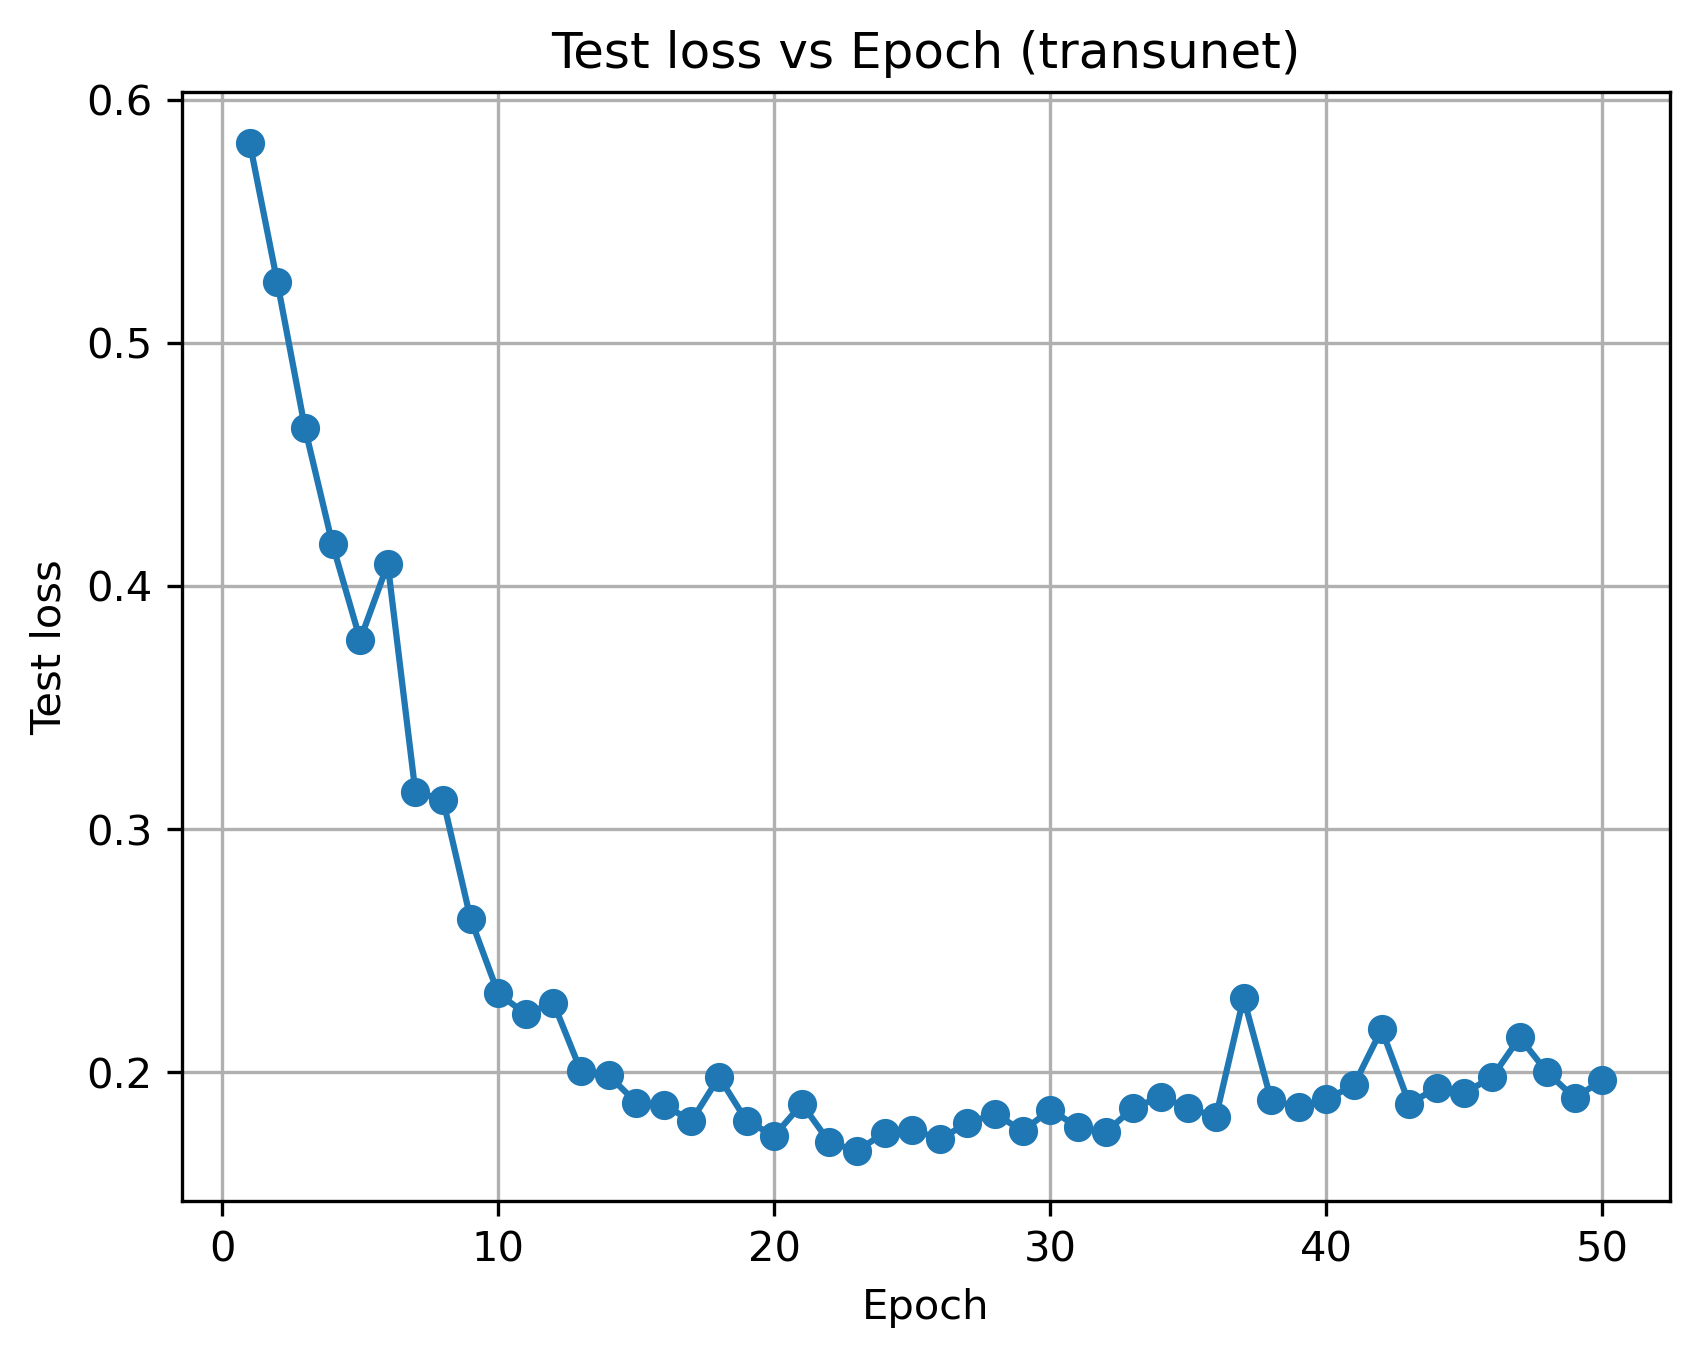
\includegraphics[width=\textwidth]{figures/test_loss_transunet_base.png}
        \caption{TransUNet}
        \label{subfig: TransUNet vs JamUNet test loss}
    \end{subfigure}
    \begin{subfigure}[b]{0.4\textwidth}
        \centering
        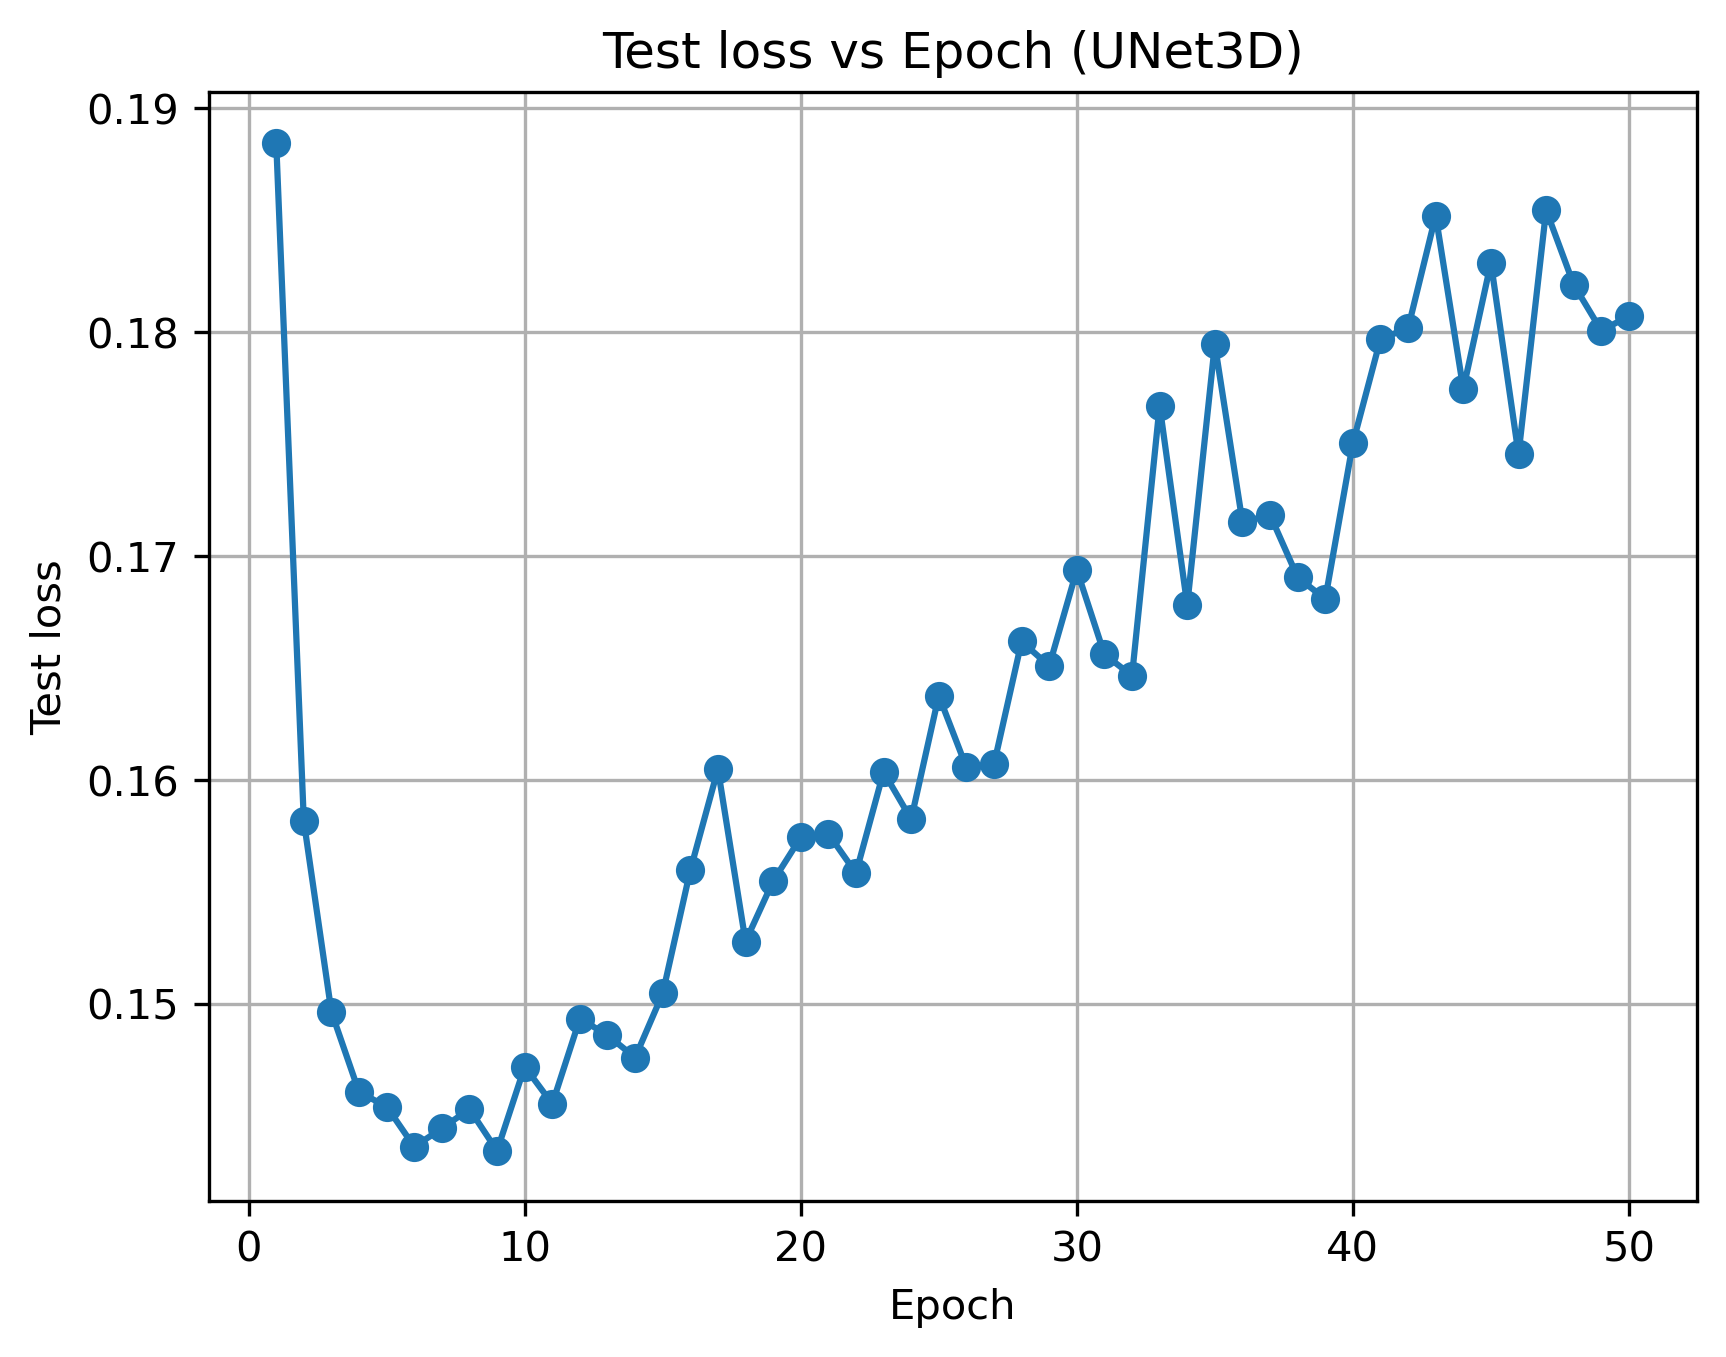
\includegraphics[width=\textwidth]{figures/test_loss_unet3d_base.png}
        \caption{JamUNet}
        \label{subfig: JamUNet test loss}
    \end{subfigure}
    \caption{Variation of test loss against training epoch.}
    \label{fig: TransUNet vs JamUNet test loss}
\end{figure}

\begin{figure}[H]
    \centering
    \begin{subfigure}[b]{0.4\textwidth}
        \centering
        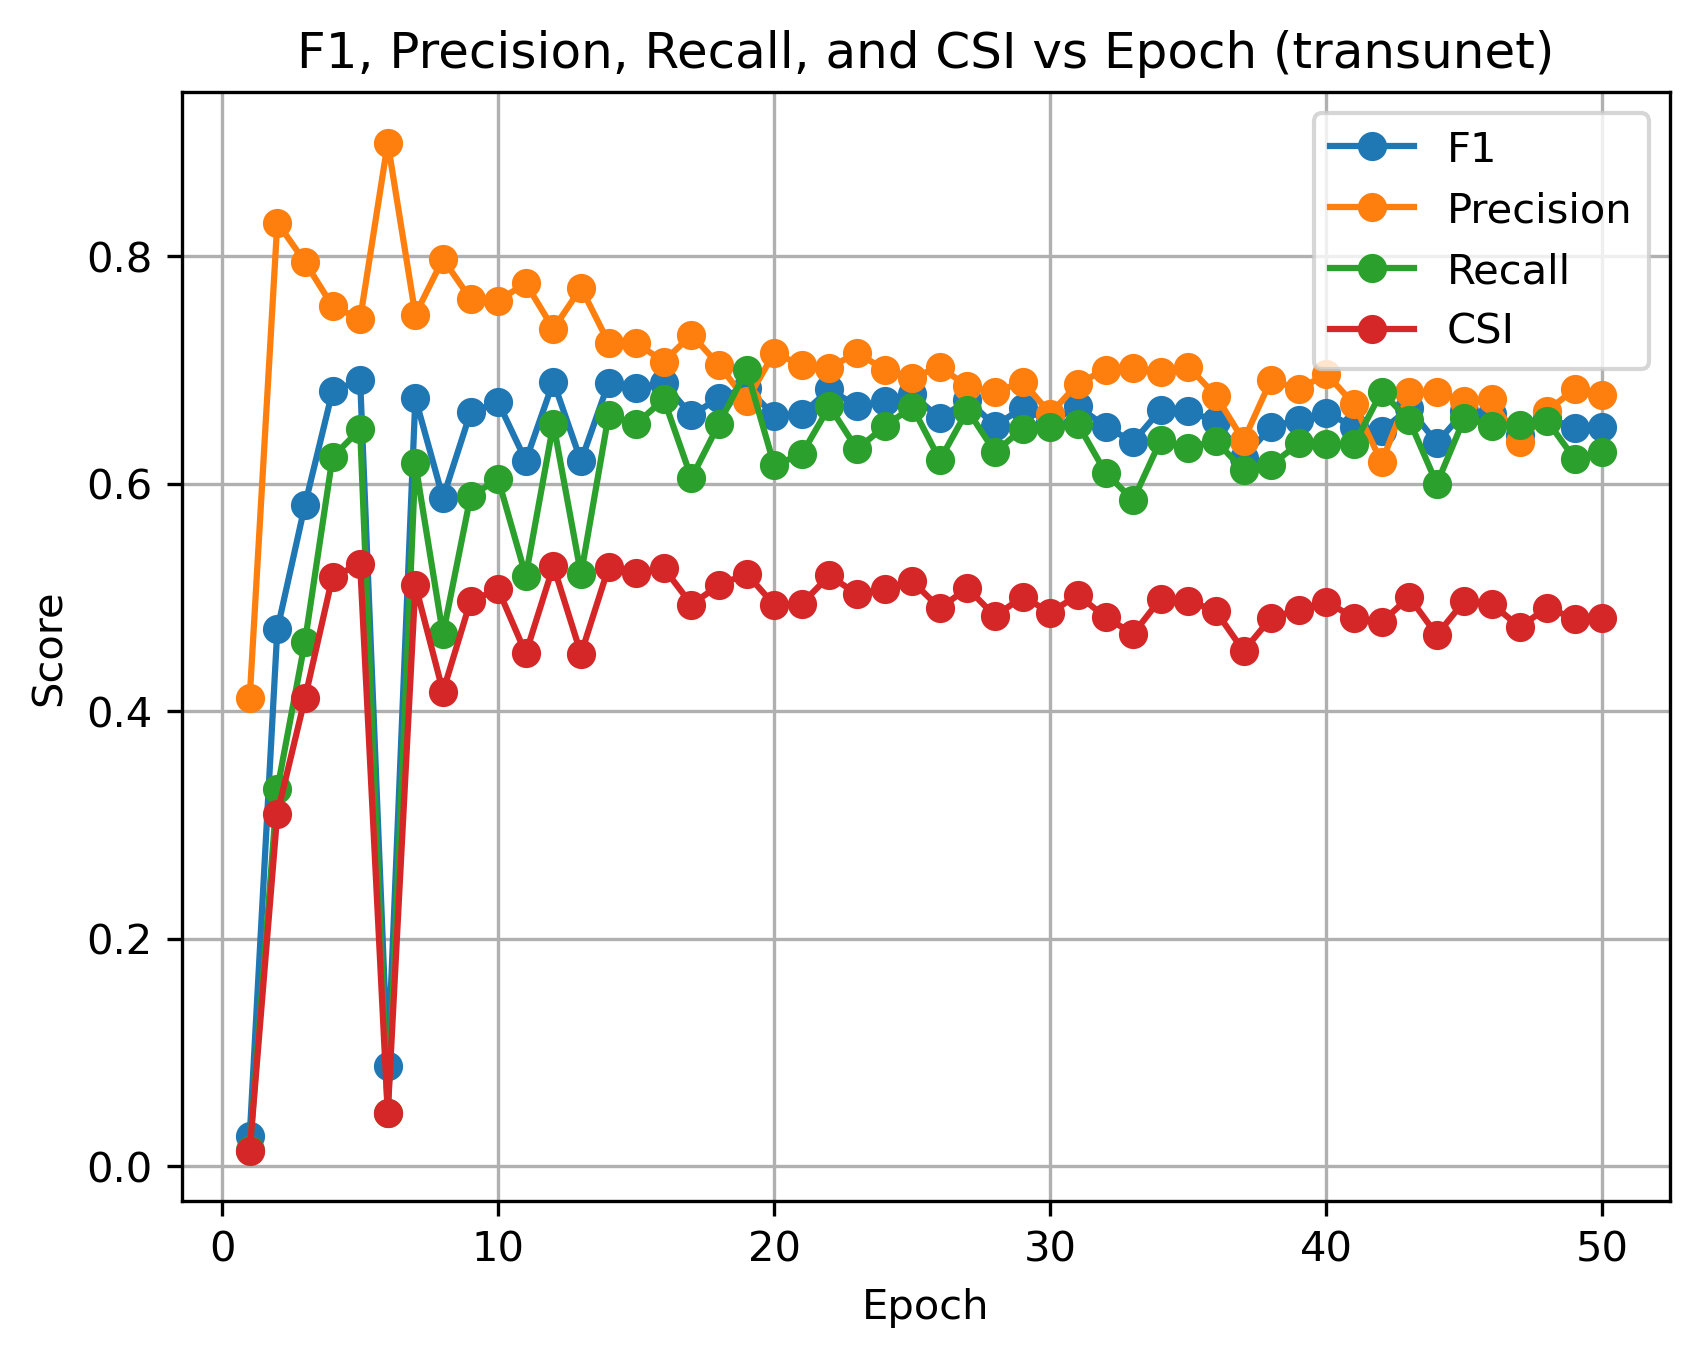
\includegraphics[width=\textwidth]{figures/test_scores_transunet_base.png}
        \caption{TransUNet}
        \label{subfig: TransUNet scores}
    \end{subfigure}
    \begin{subfigure}[b]{0.4\textwidth}
        \centering
        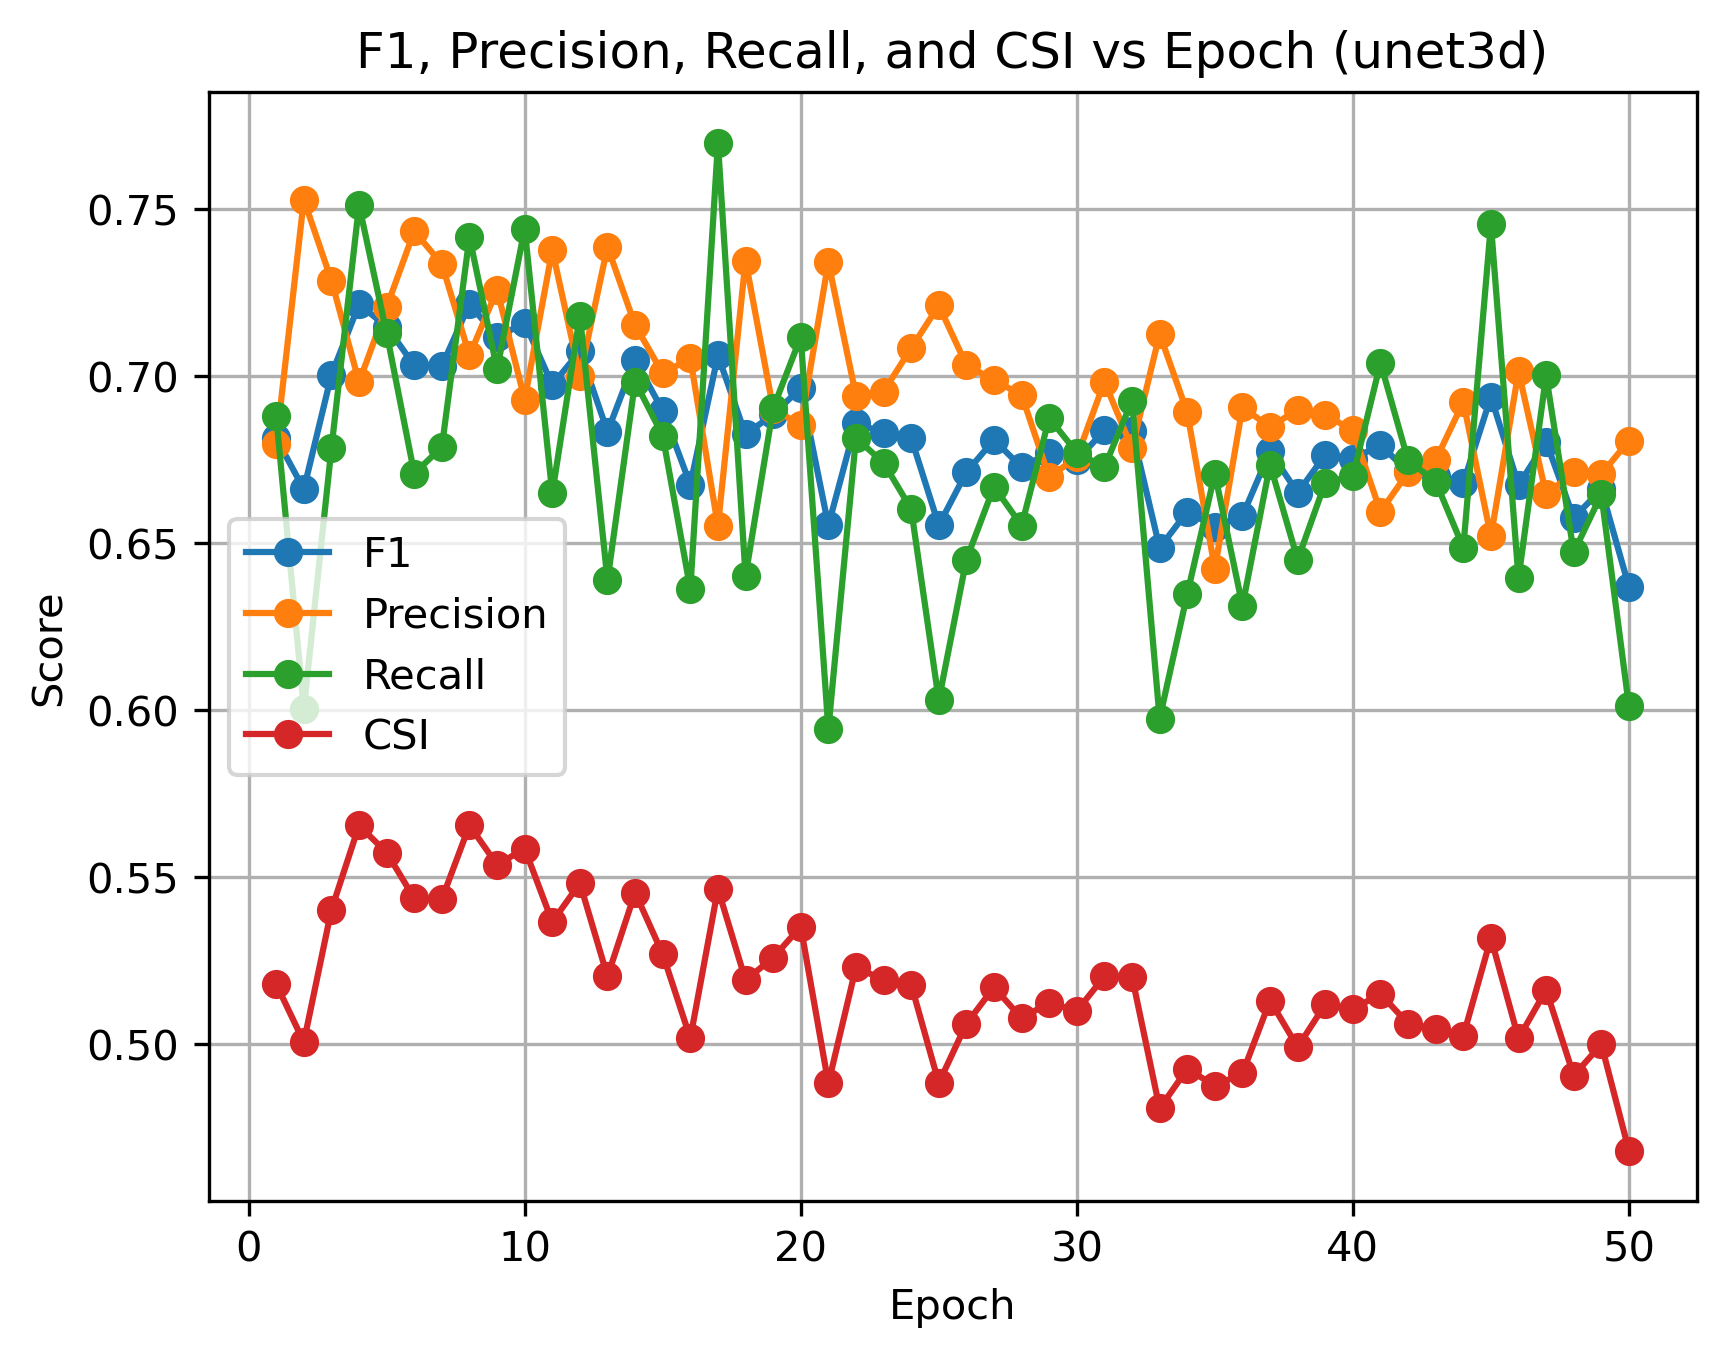
\includegraphics[width=\textwidth]{figures/test_scores_unet3d_base.png}
        \caption{JamUNet}
        \label{subfig: JamUNet scores}
    \end{subfigure}
    \caption{F1, recall, precision, csi scores comparison between TransUNet and JamUNet models.}
    \label{fig: TransUNet vs JamUNet scores comparison}
\end{figure}

\begin{figure}[H]
    \centering
    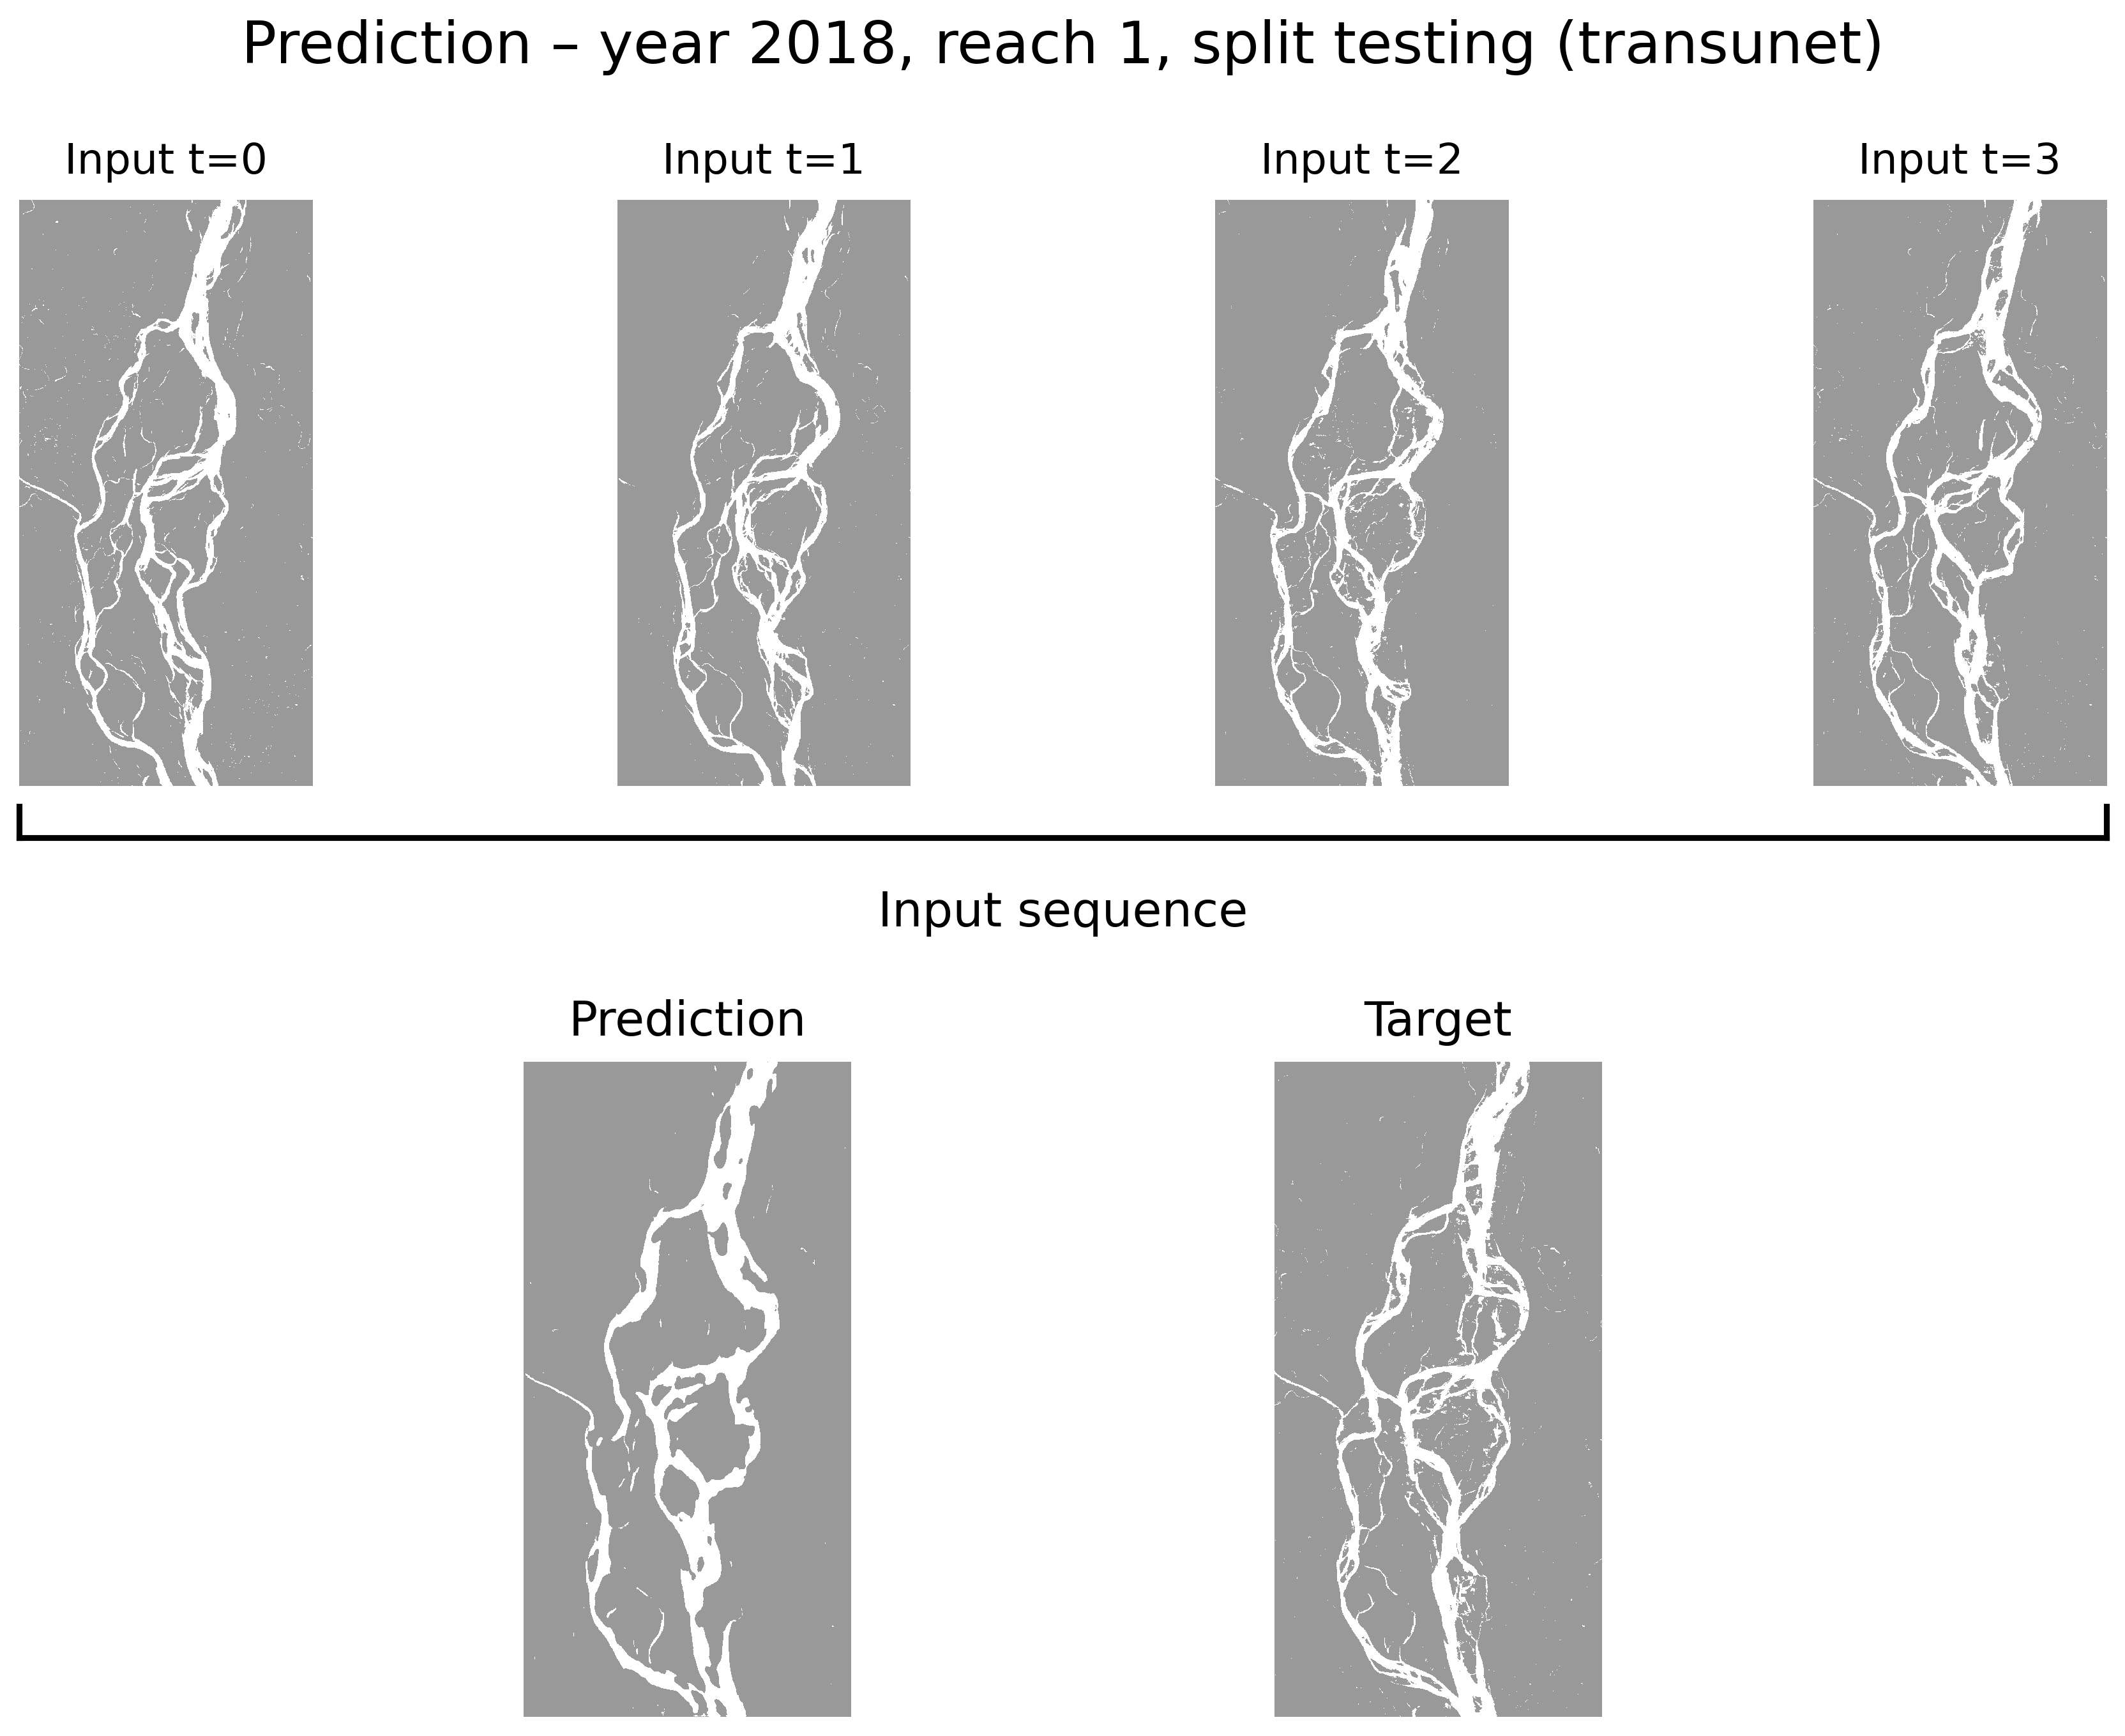
\includegraphics[width=0.75\linewidth]{figures/prediction_year2018_reach1_testing_transunet_base_epoch019.png}
    \caption{TransUNet input sequence of years $2014-2017$, target year $2018$ for sample river location.}
    \label{fig: TransUNet prediction map}
\end{figure}

\begin{figure}[H]
    \centering
    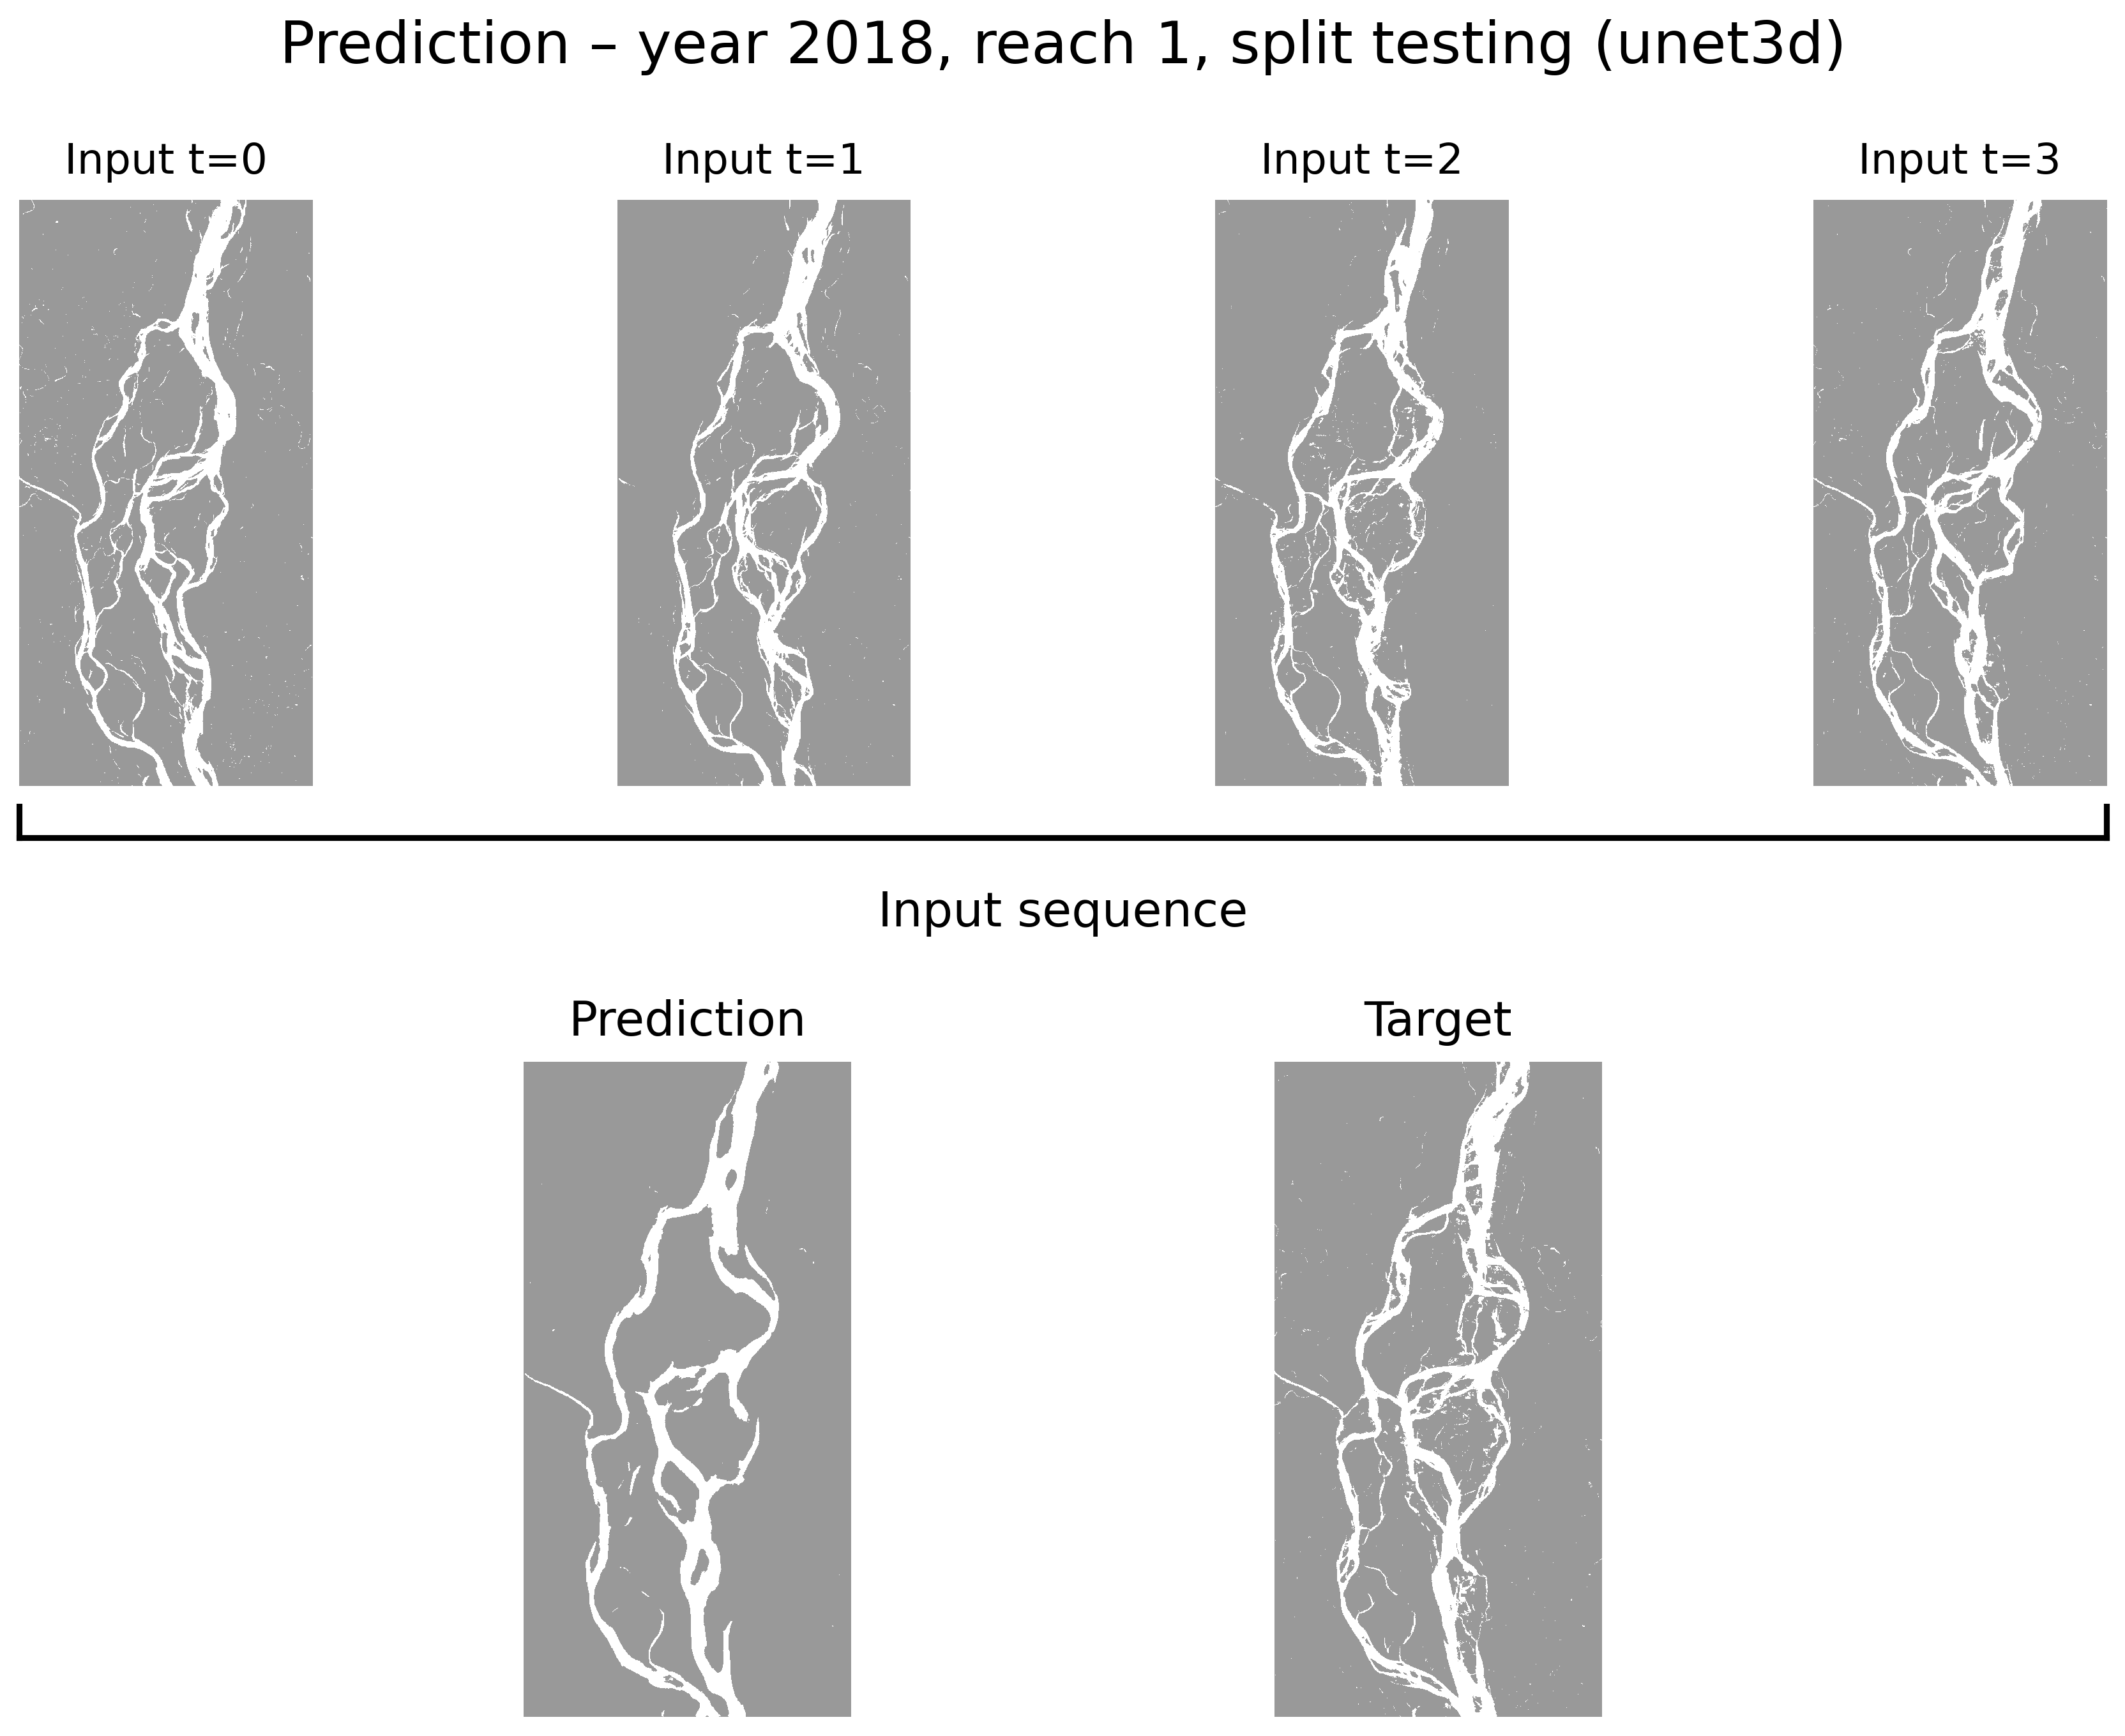
\includegraphics[width=0.75\linewidth]{figures/prediction_year2018_reach1_testing_unet3d_base_epoch009.png}
    \caption{JamUNet input sequence of years $2014-2017$, target year $2018$ for sample river location.}
    \label{fig: JamUNet prediction map}
\end{figure}

\begin{figure}[H]
    \centering
    \begin{subfigure}[b]{0.495\textwidth}
        \centering
        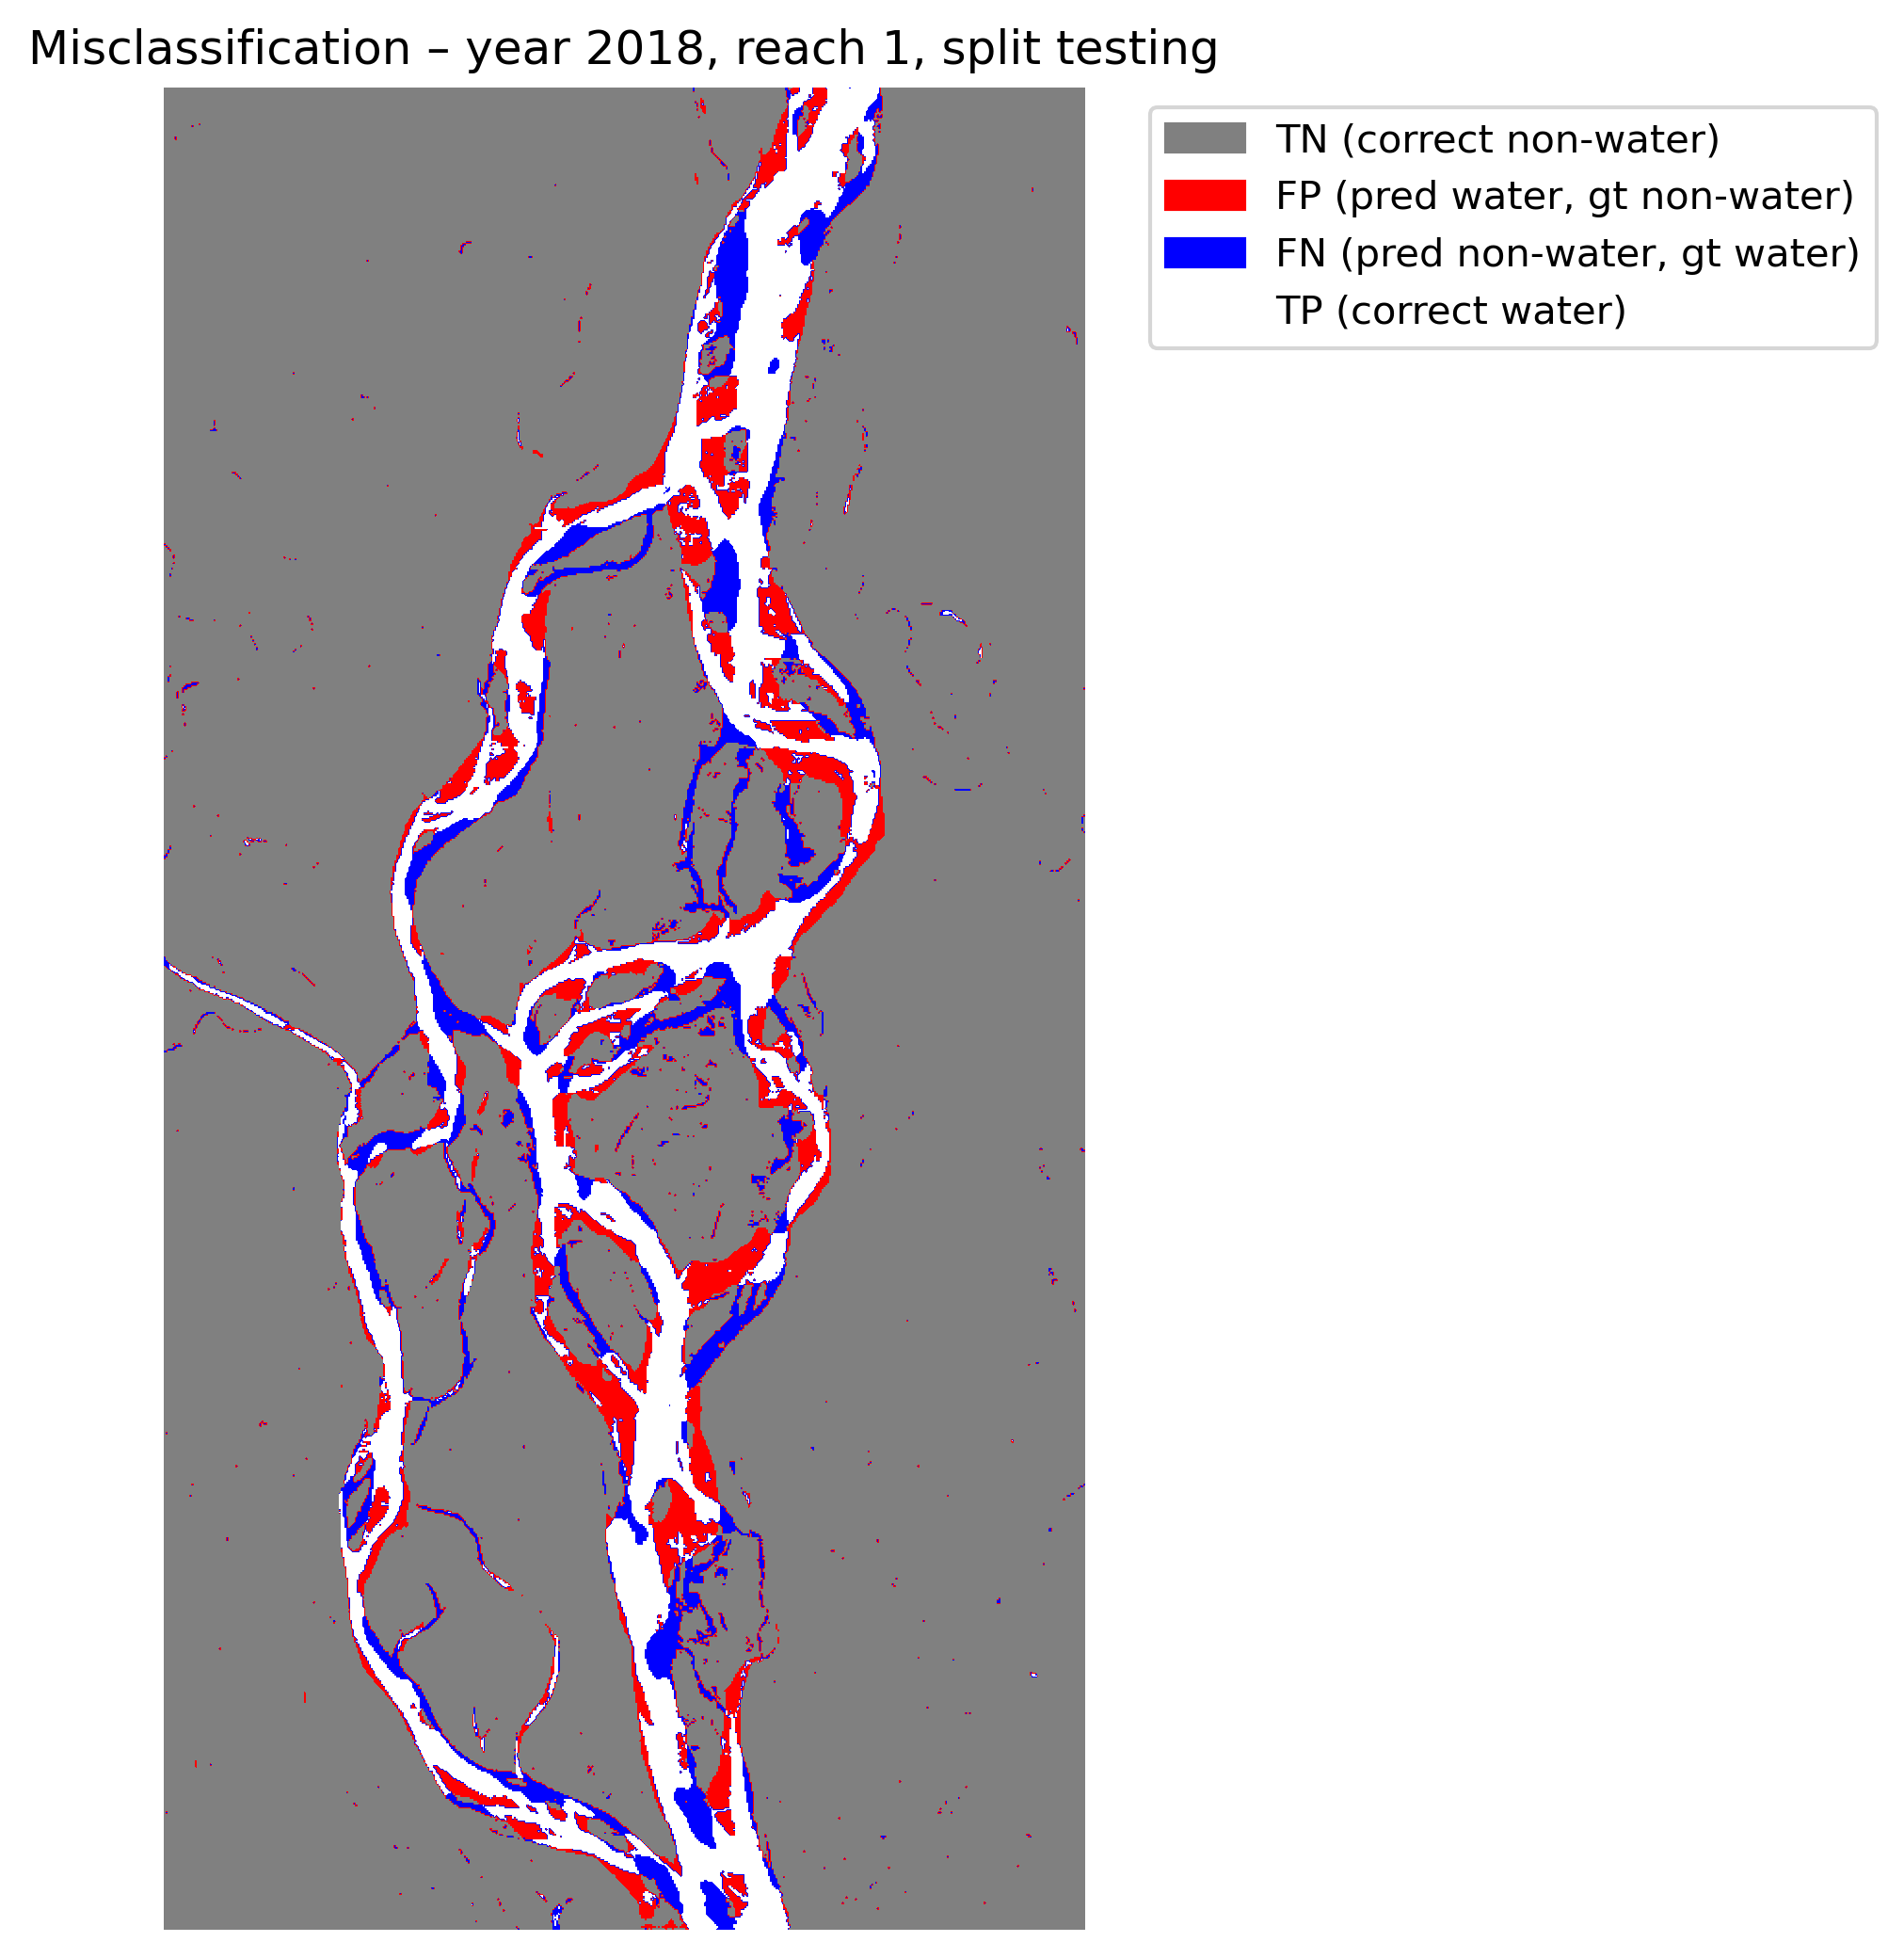
\includegraphics[width=\textwidth]{figures/misclass_year2018_reach1_testing_transunet_base_epoch019.png}
        \caption{TransUNet}
        \label{subfig: TransUNet misclassification map}
    \end{subfigure}
    \begin{subfigure}[b]{0.495\textwidth}
        \centering
        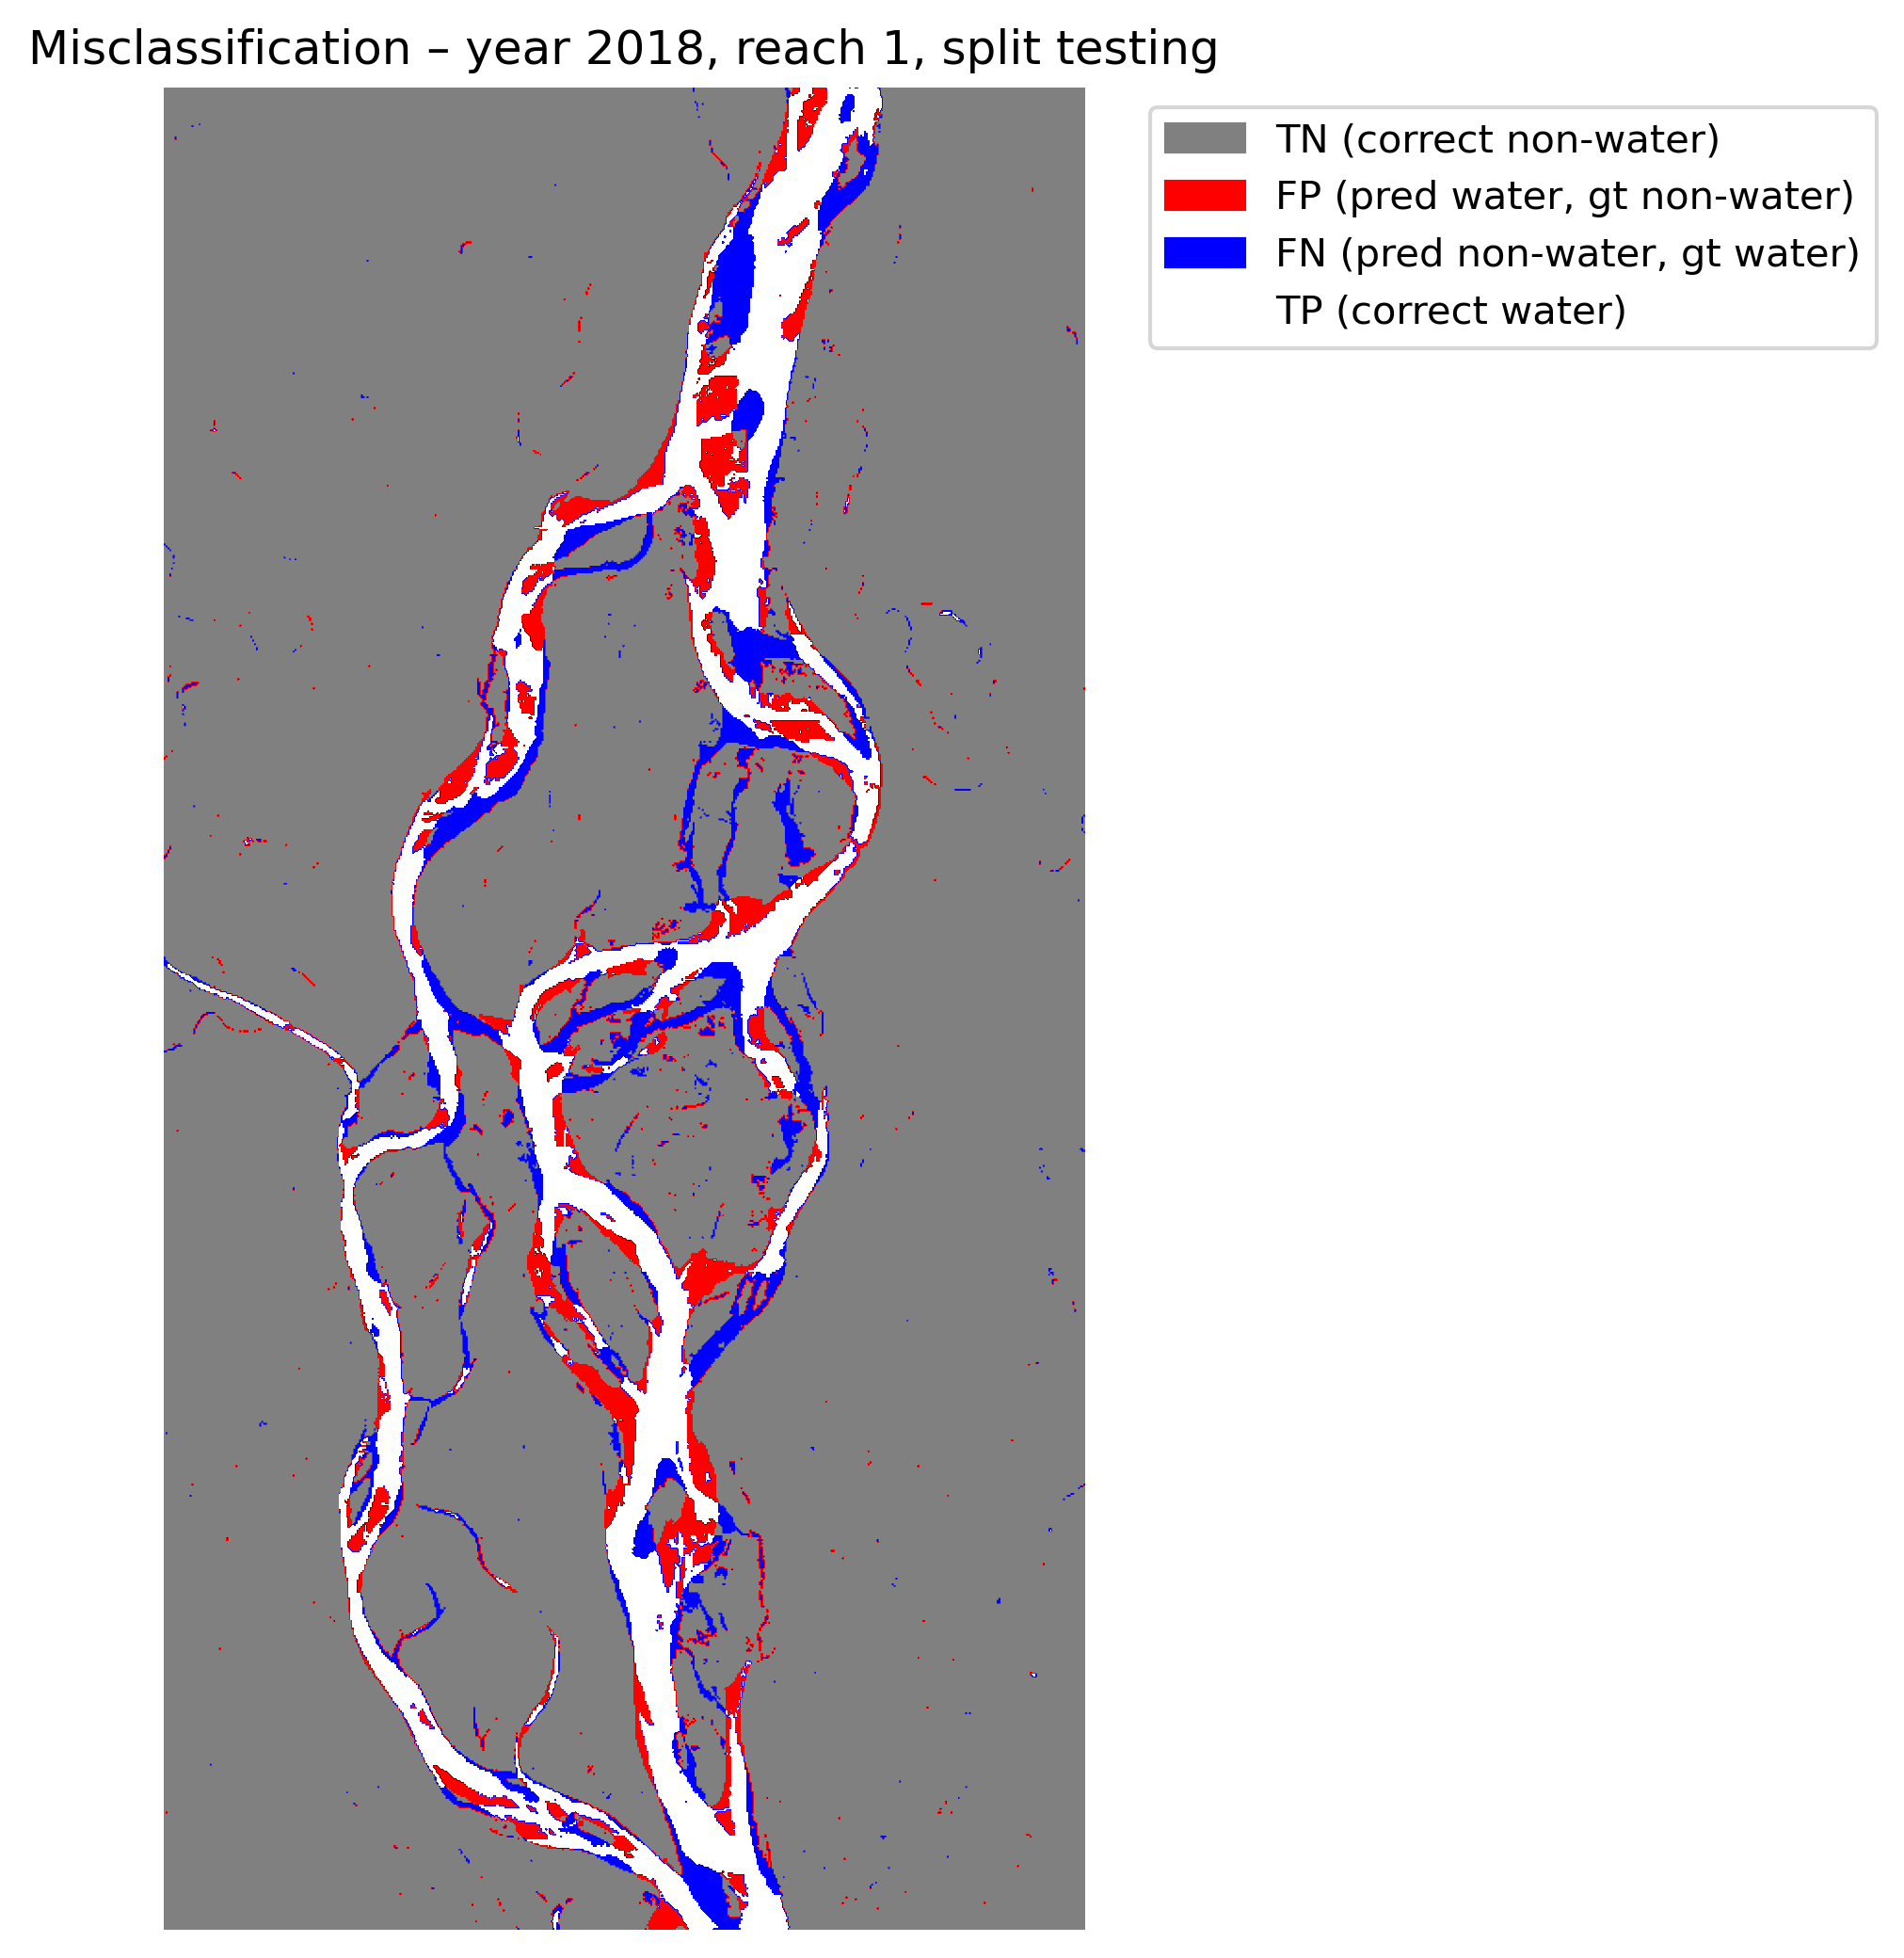
\includegraphics[width=\textwidth]{figures/misclass_year2018_reach1_testing_unet3d_base_epoch009.png}
        \caption{JamUNet}
        \label{subfig: JamUNet misclassification map}
    \end{subfigure}
    \caption{Misclassification map comparison between TransUNet and JamUNet models on a selected test image.}
    \label{fig: TransUNet vs JamUNet misclassification map}
\end{figure}

\begin{figure}[H]
    \centering
    \begin{subfigure}[b]{0.4\textwidth}
        \centering
        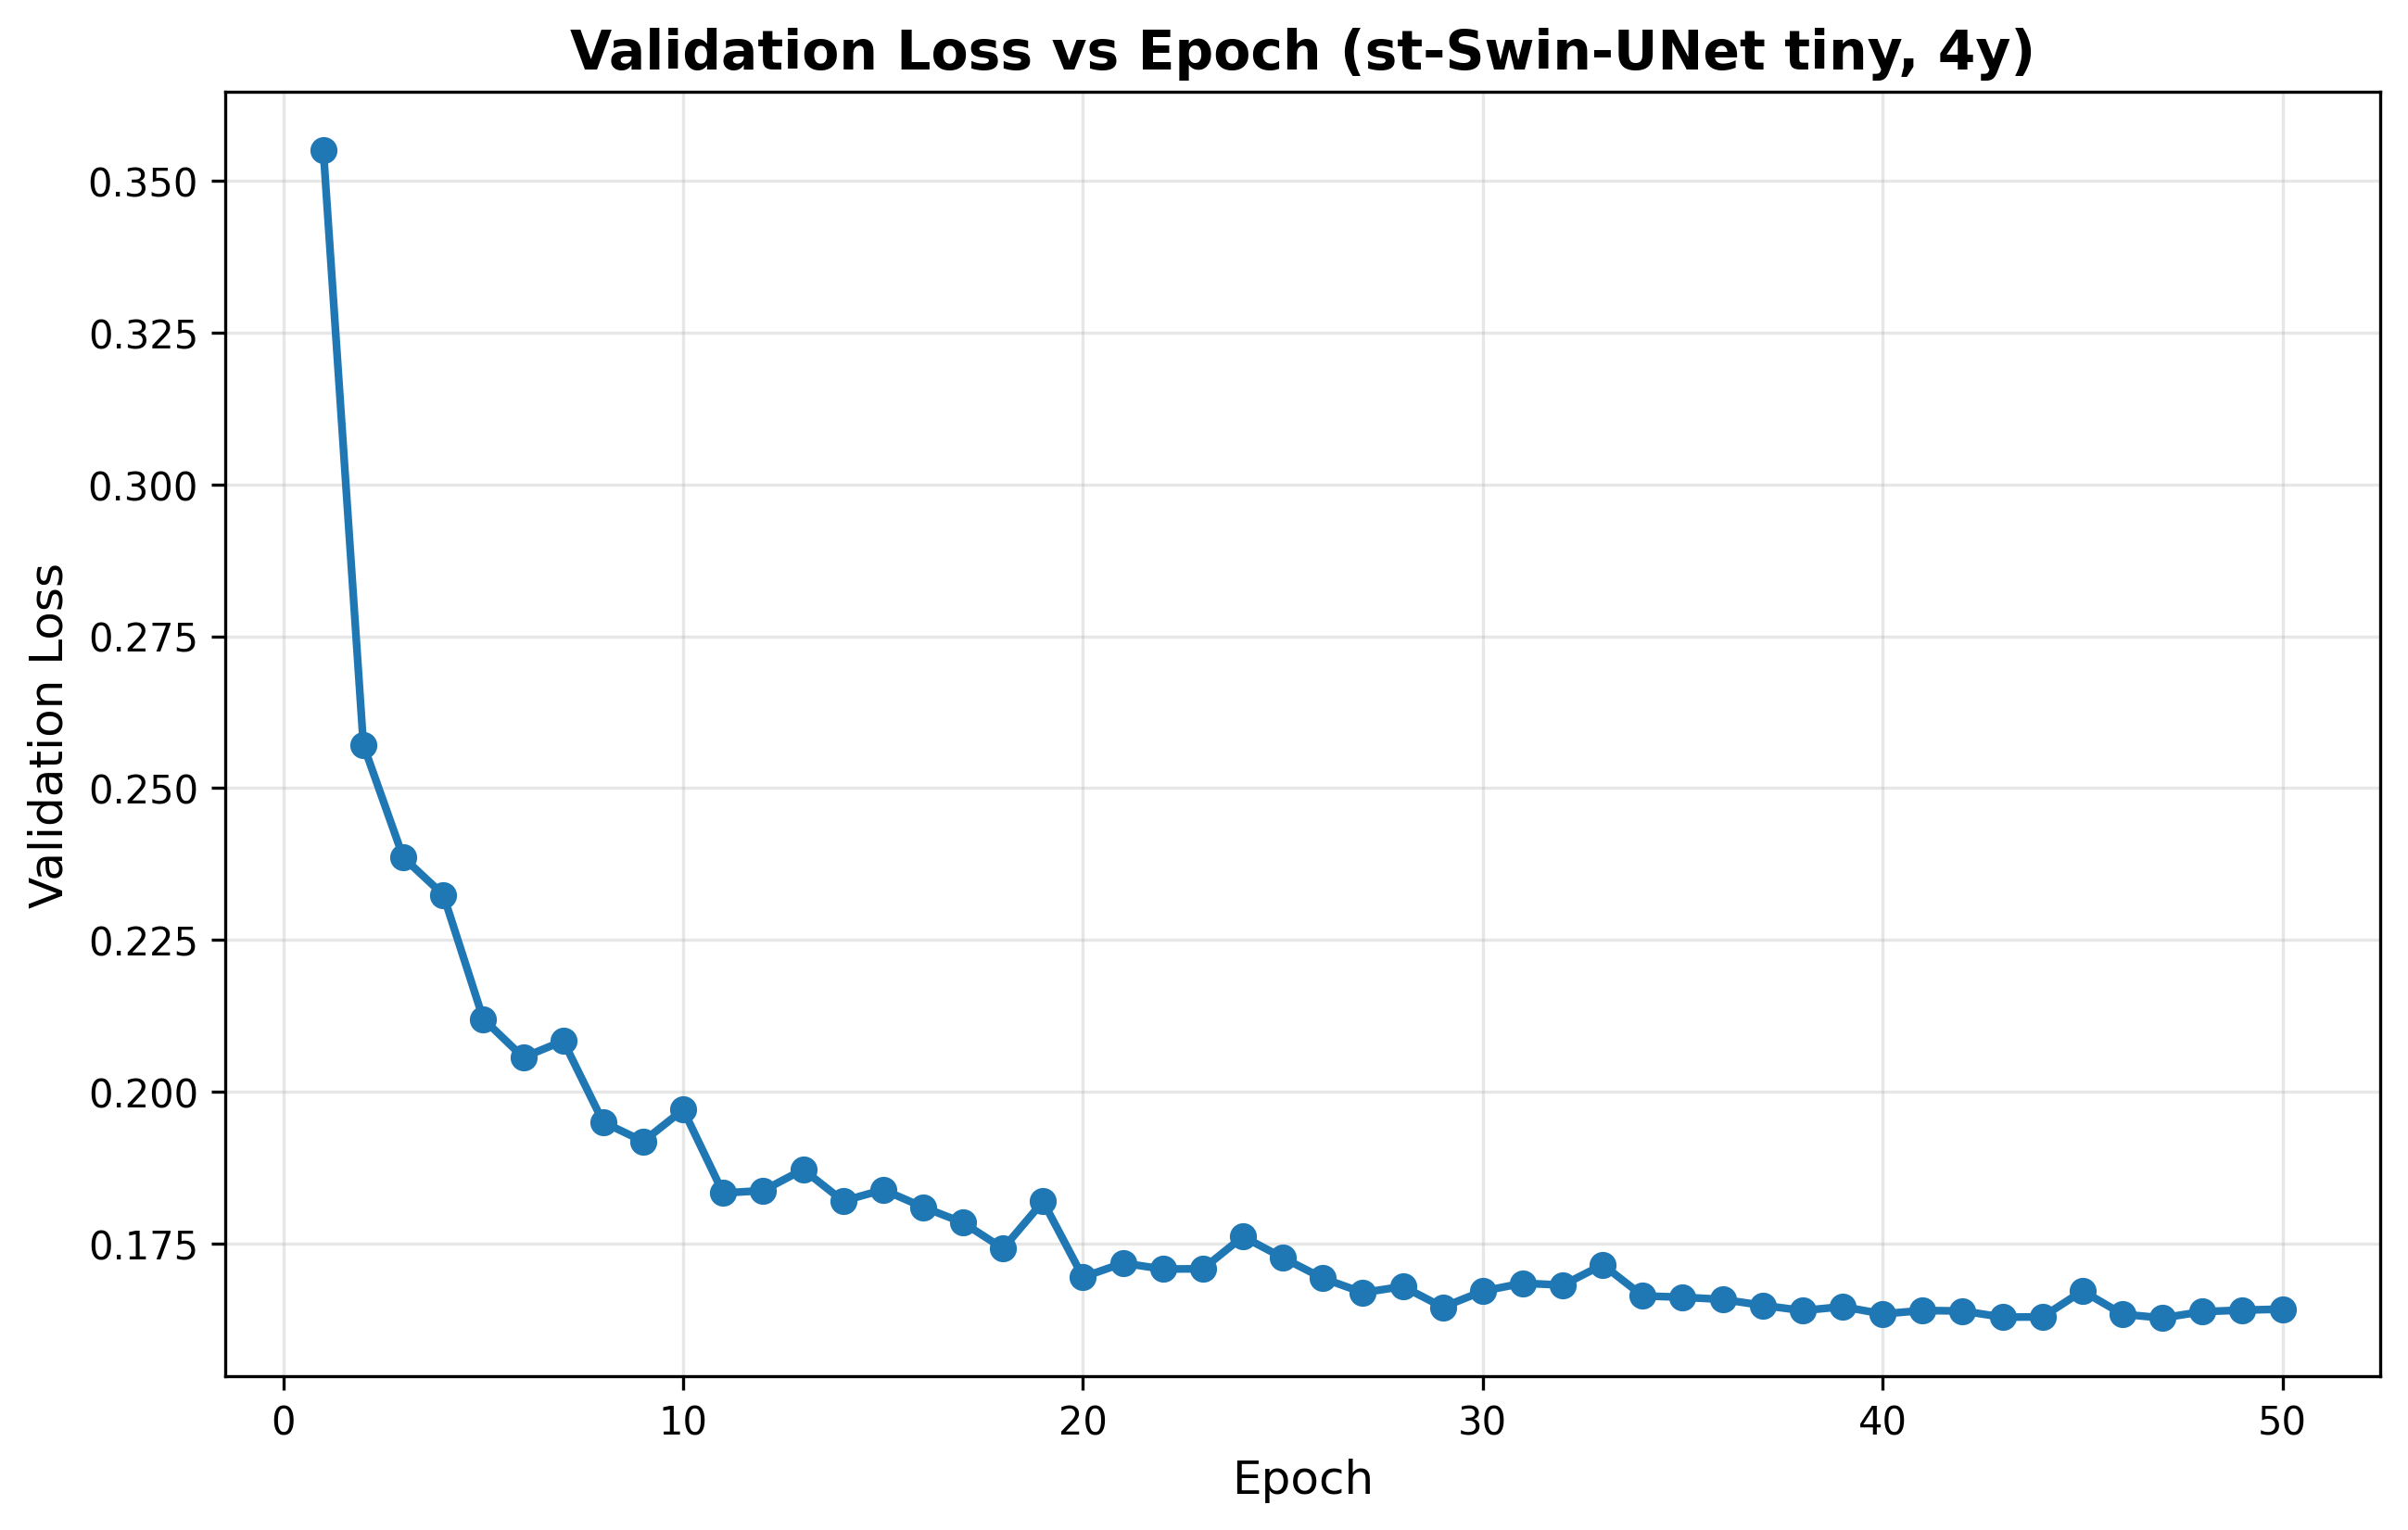
\includegraphics[width=\textwidth]{figures/val_loss_stswin_tiny_4y.png}
        \caption{st-Swin-UNet Tiny}
        \label{subfig: st-Swin-UNet tiny validation loss}
    \end{subfigure}
    \begin{subfigure}[b]{0.4\textwidth}
        \centering
        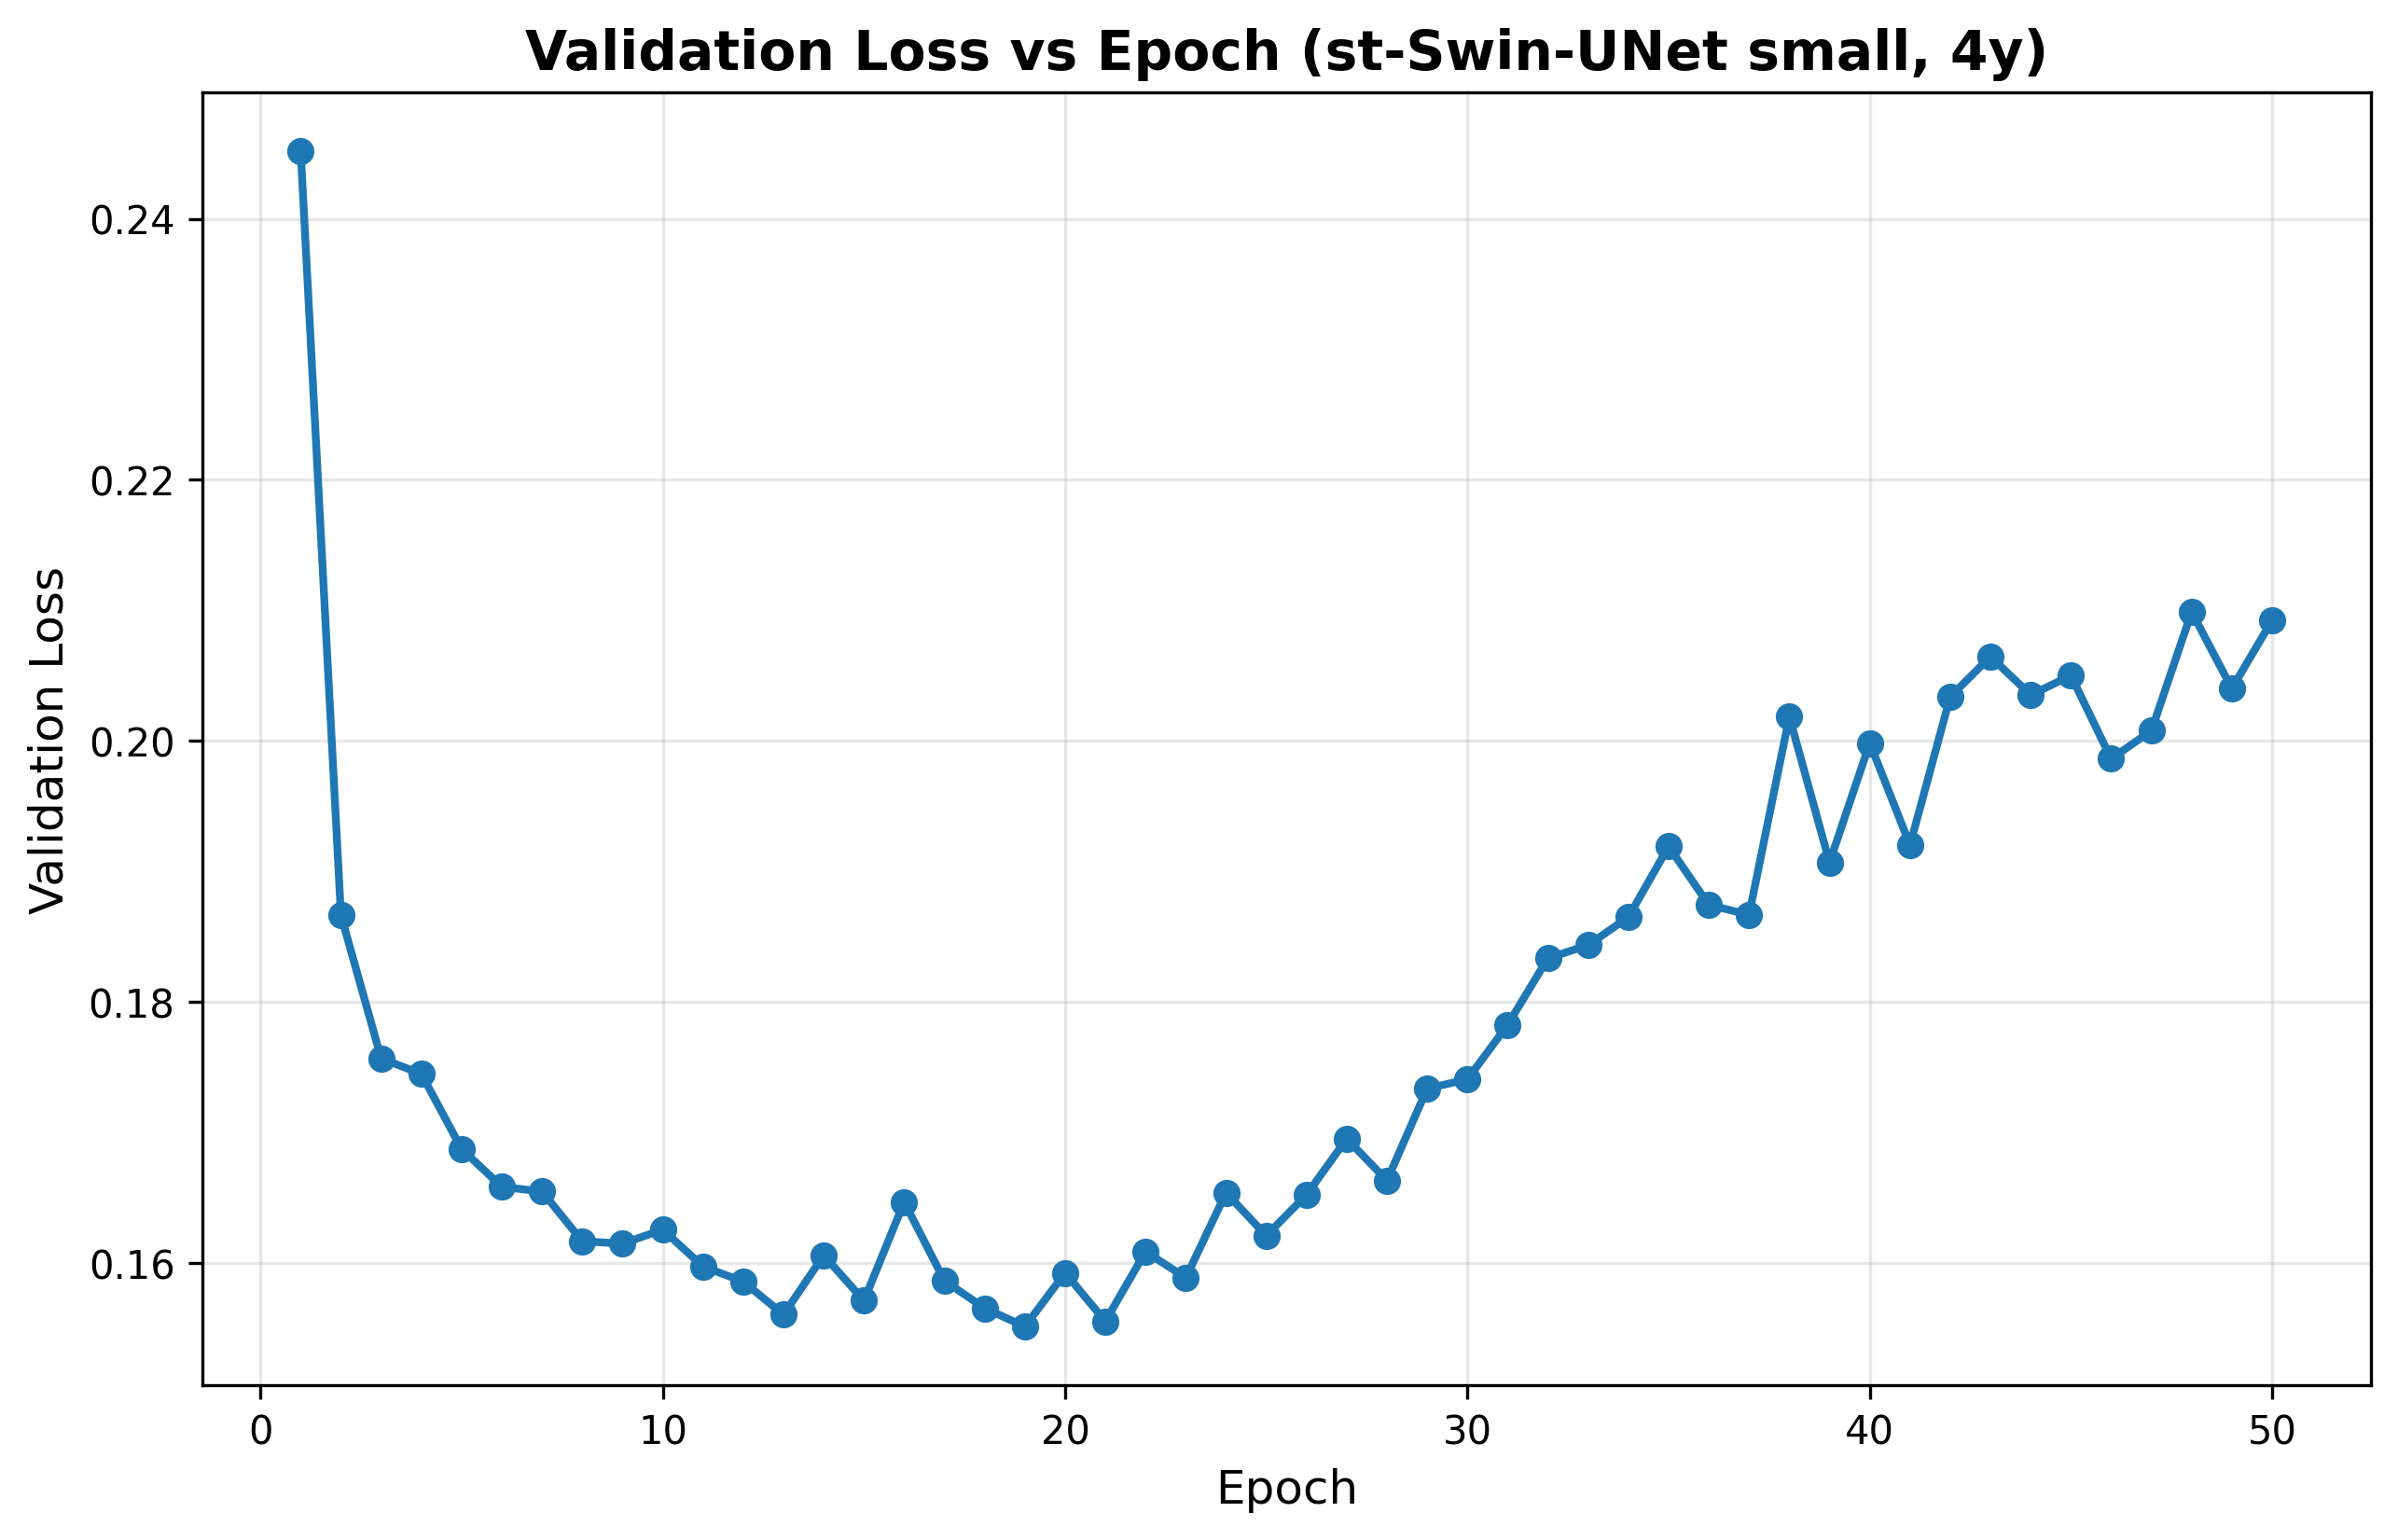
\includegraphics[width=\textwidth]{figures/val_loss_stswin_small_4y.png}
        \caption{st-Swin-UNet Small}
        \label{subfig: st-Swin-UNet small validation loss}
    \end{subfigure}
    \caption{Validation loss vs epoch for st-Swin-UNet variants ($4$-year input).}
    \label{fig: st-Swin-UNet validation loss}
\end{figure}

\begin{figure}[H]
    \centering
    \begin{subfigure}[b]{0.4\textwidth}
        \centering
        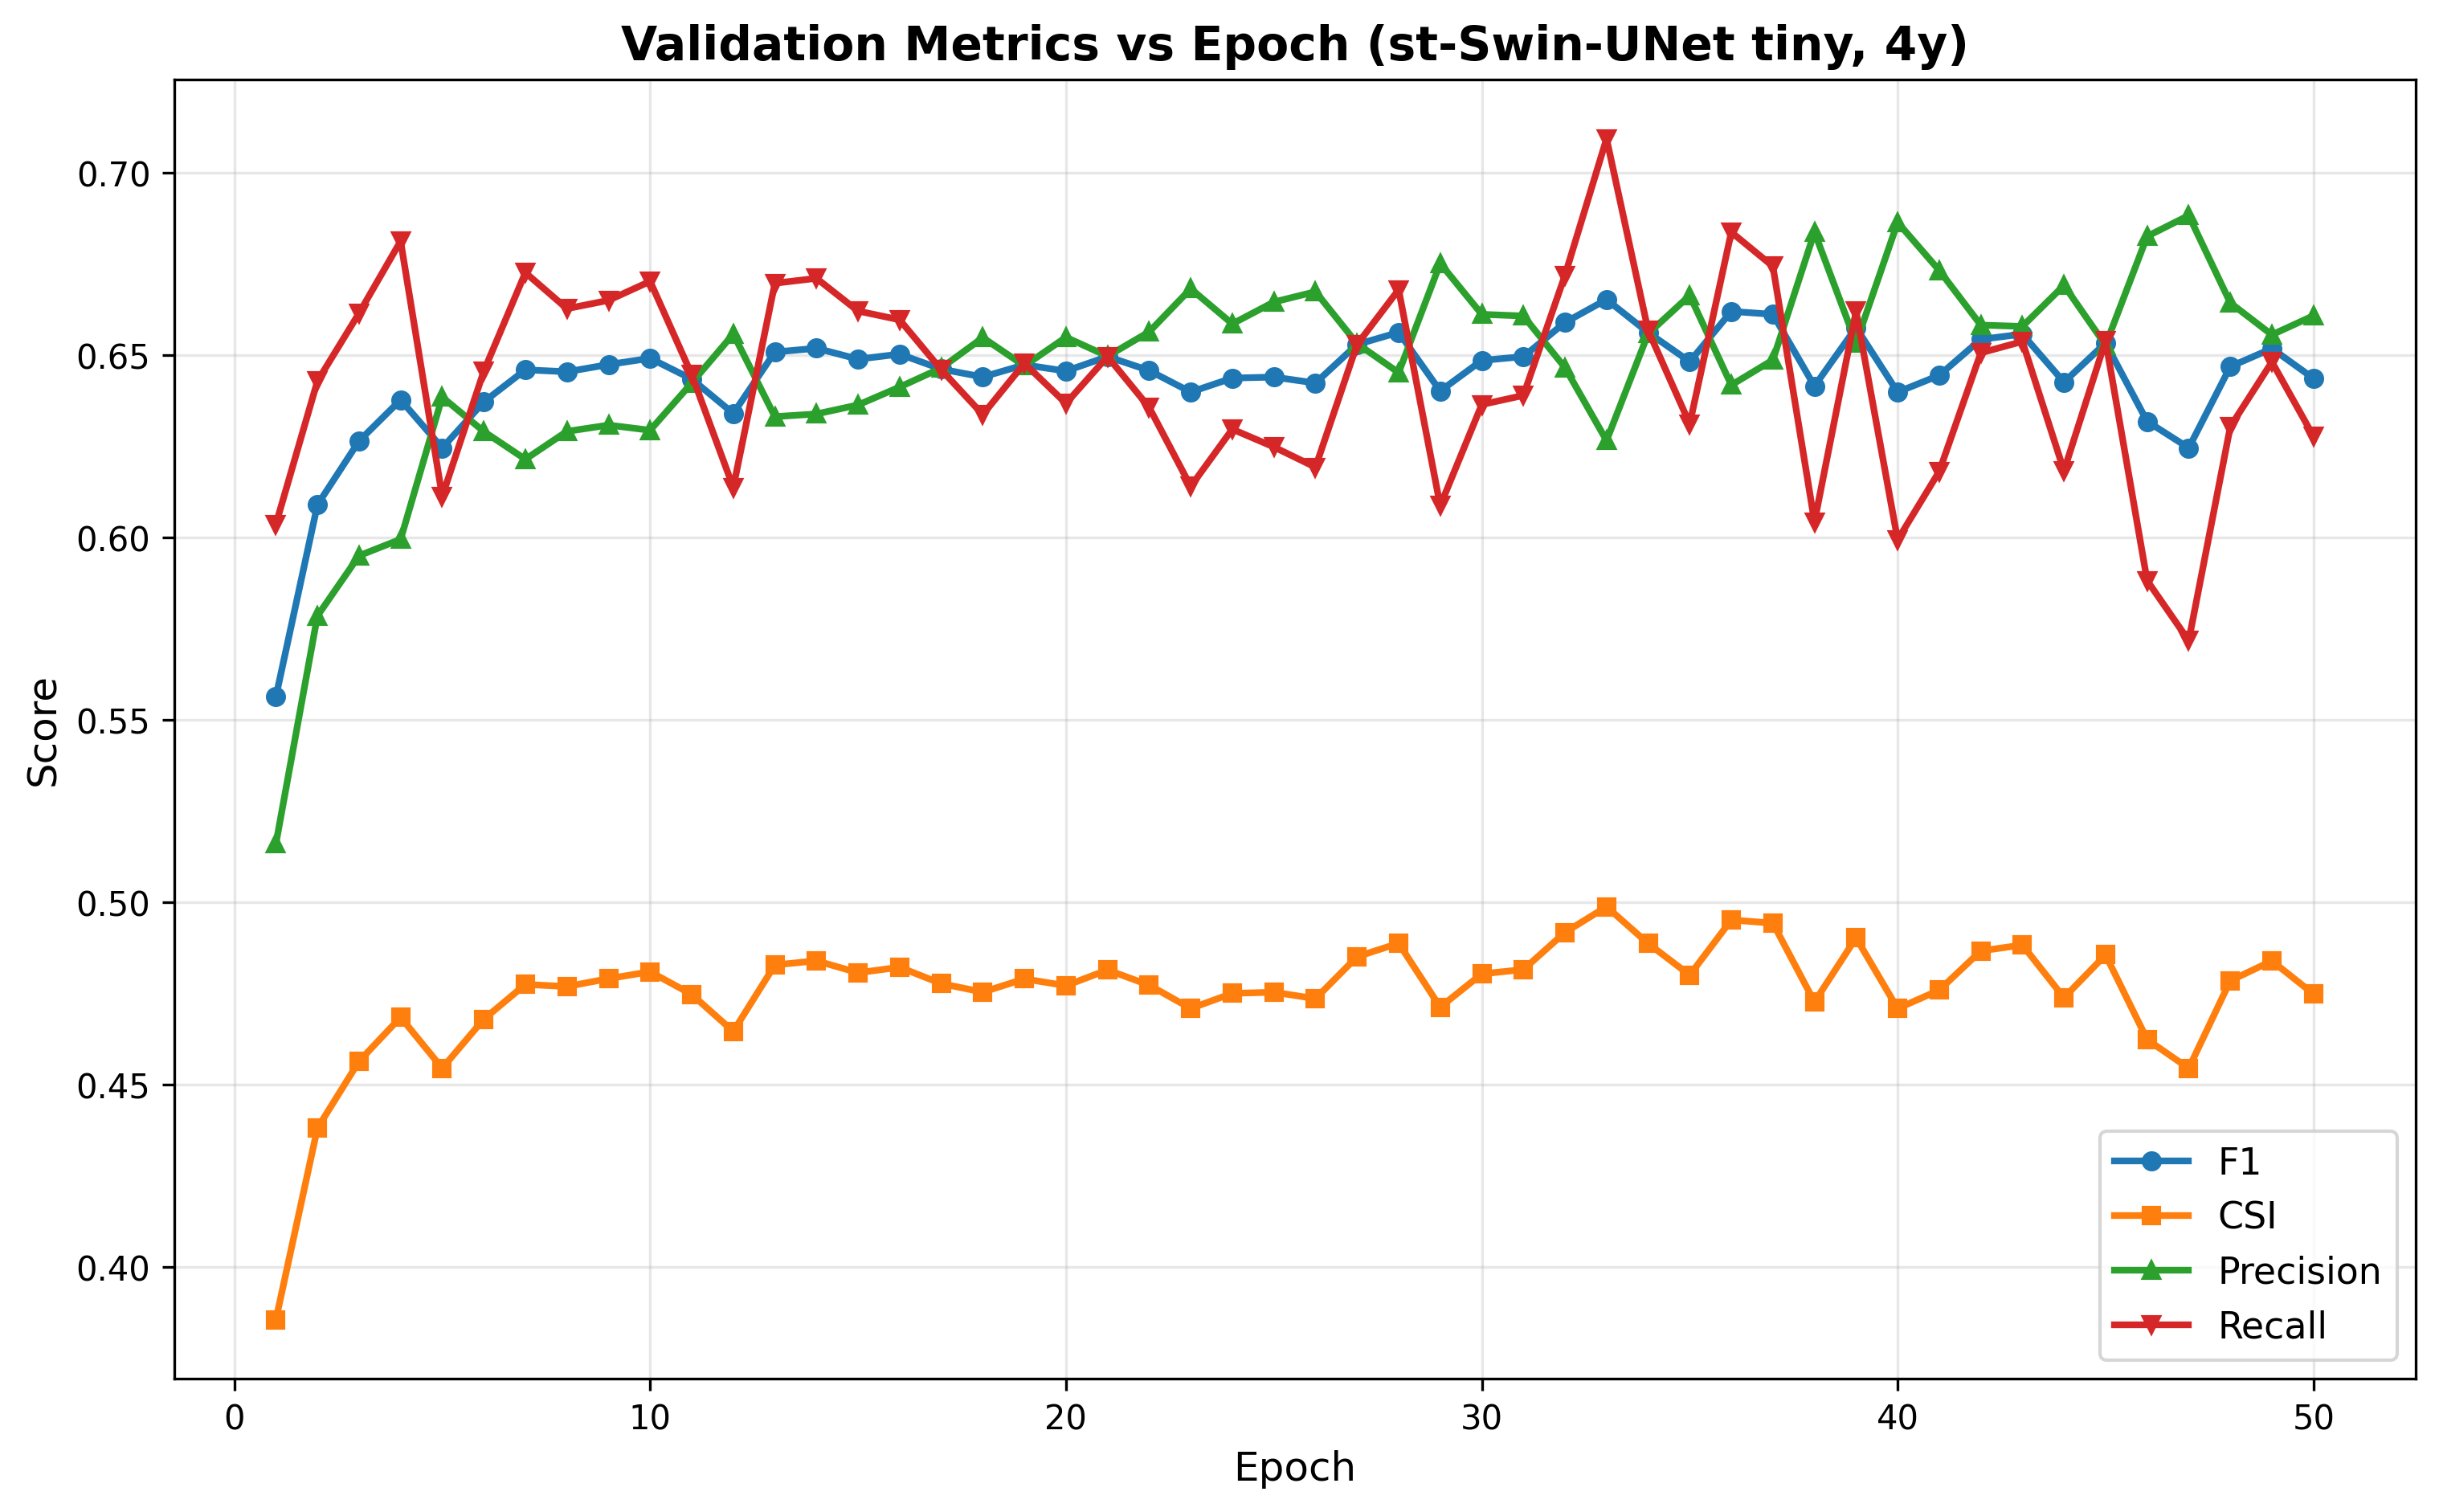
\includegraphics[width=\textwidth]{figures/val_metrics_stswin_tiny_4y.png}
        \caption{st-Swin-UNet Tiny}
        \label{subfig: st-Swin-UNet tiny validation metrics}
    \end{subfigure}
    \begin{subfigure}[b]{0.4\textwidth}
        \centering
        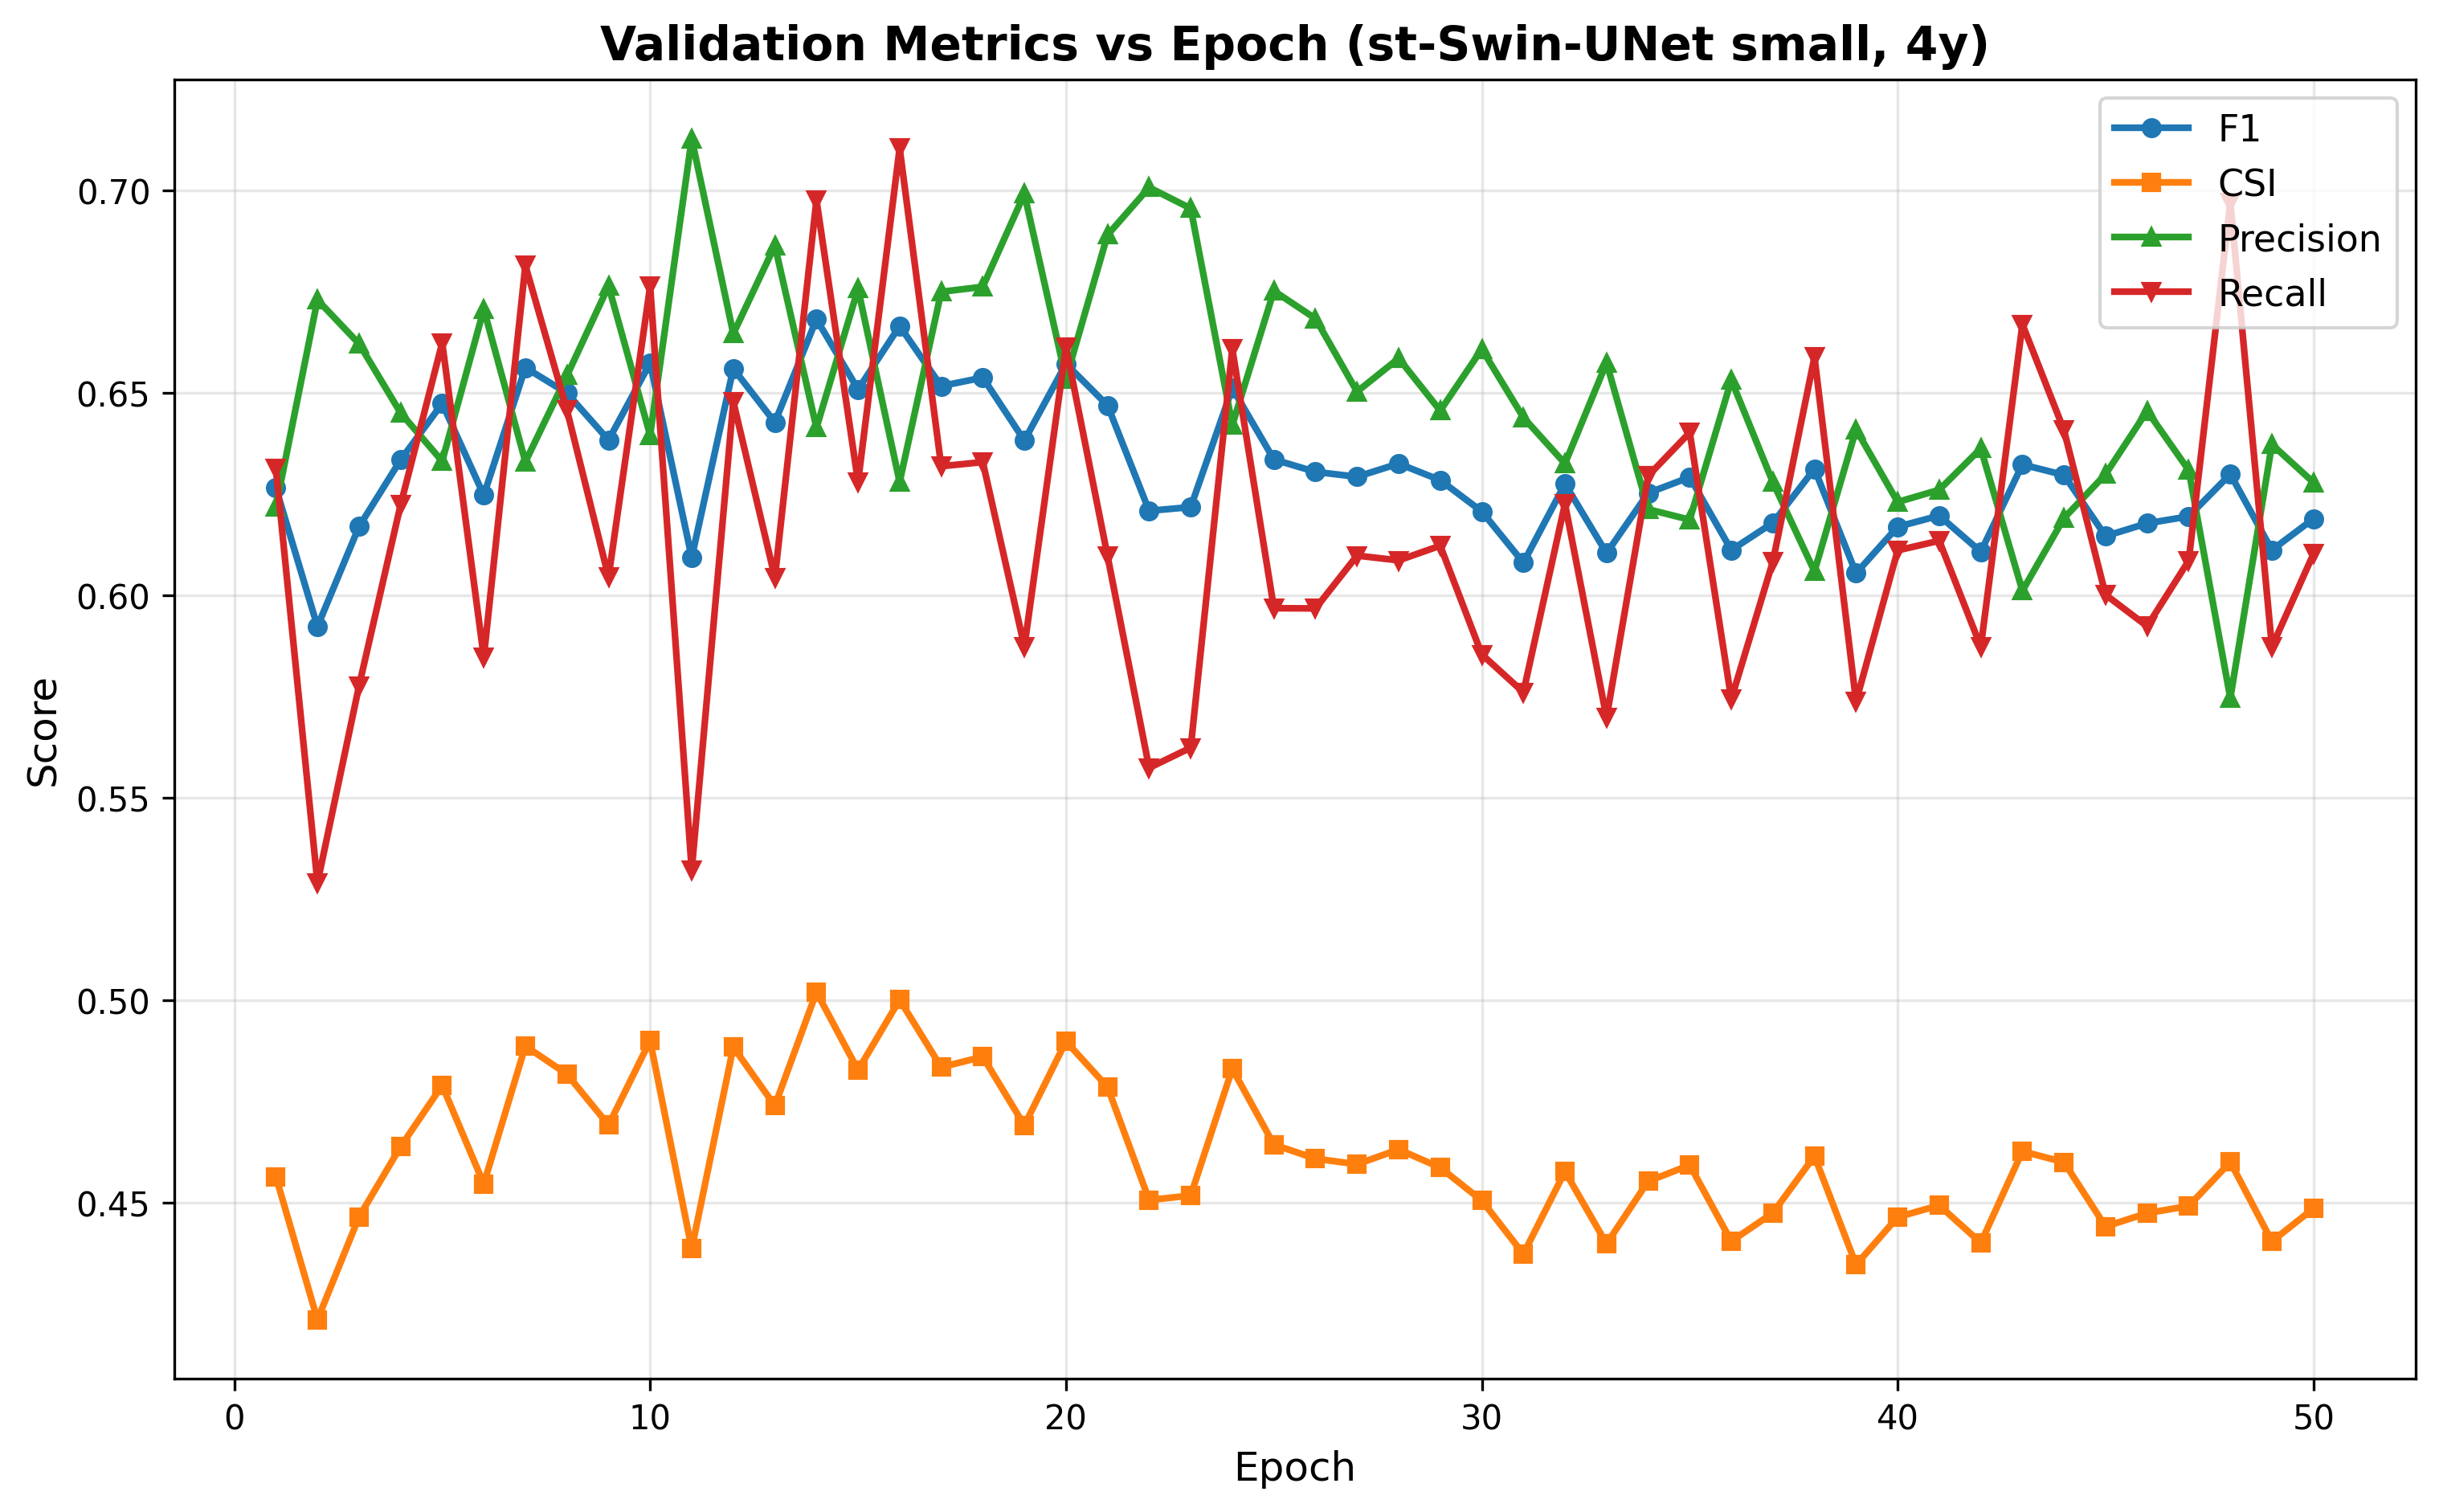
\includegraphics[width=\textwidth]{figures/val_metrics_stswin_small_4y.png}
        \caption{st-Swin-UNet Small}
        \label{subfig: st-Swin-UNet small validation metrics}
    \end{subfigure}
    \caption{F1, CSI, precision, and recall scores comparison for st-Swin-UNet variants ($4$-year input). Best checkpoints: tiny at epoch $33$ (F1 $= 0.665$), small at epoch $14$ (F1 $= 0.668$).}
    \label{fig: st-Swin-UNet validation metrics}
\end{figure}

\begin{figure}[H]
    \centering
    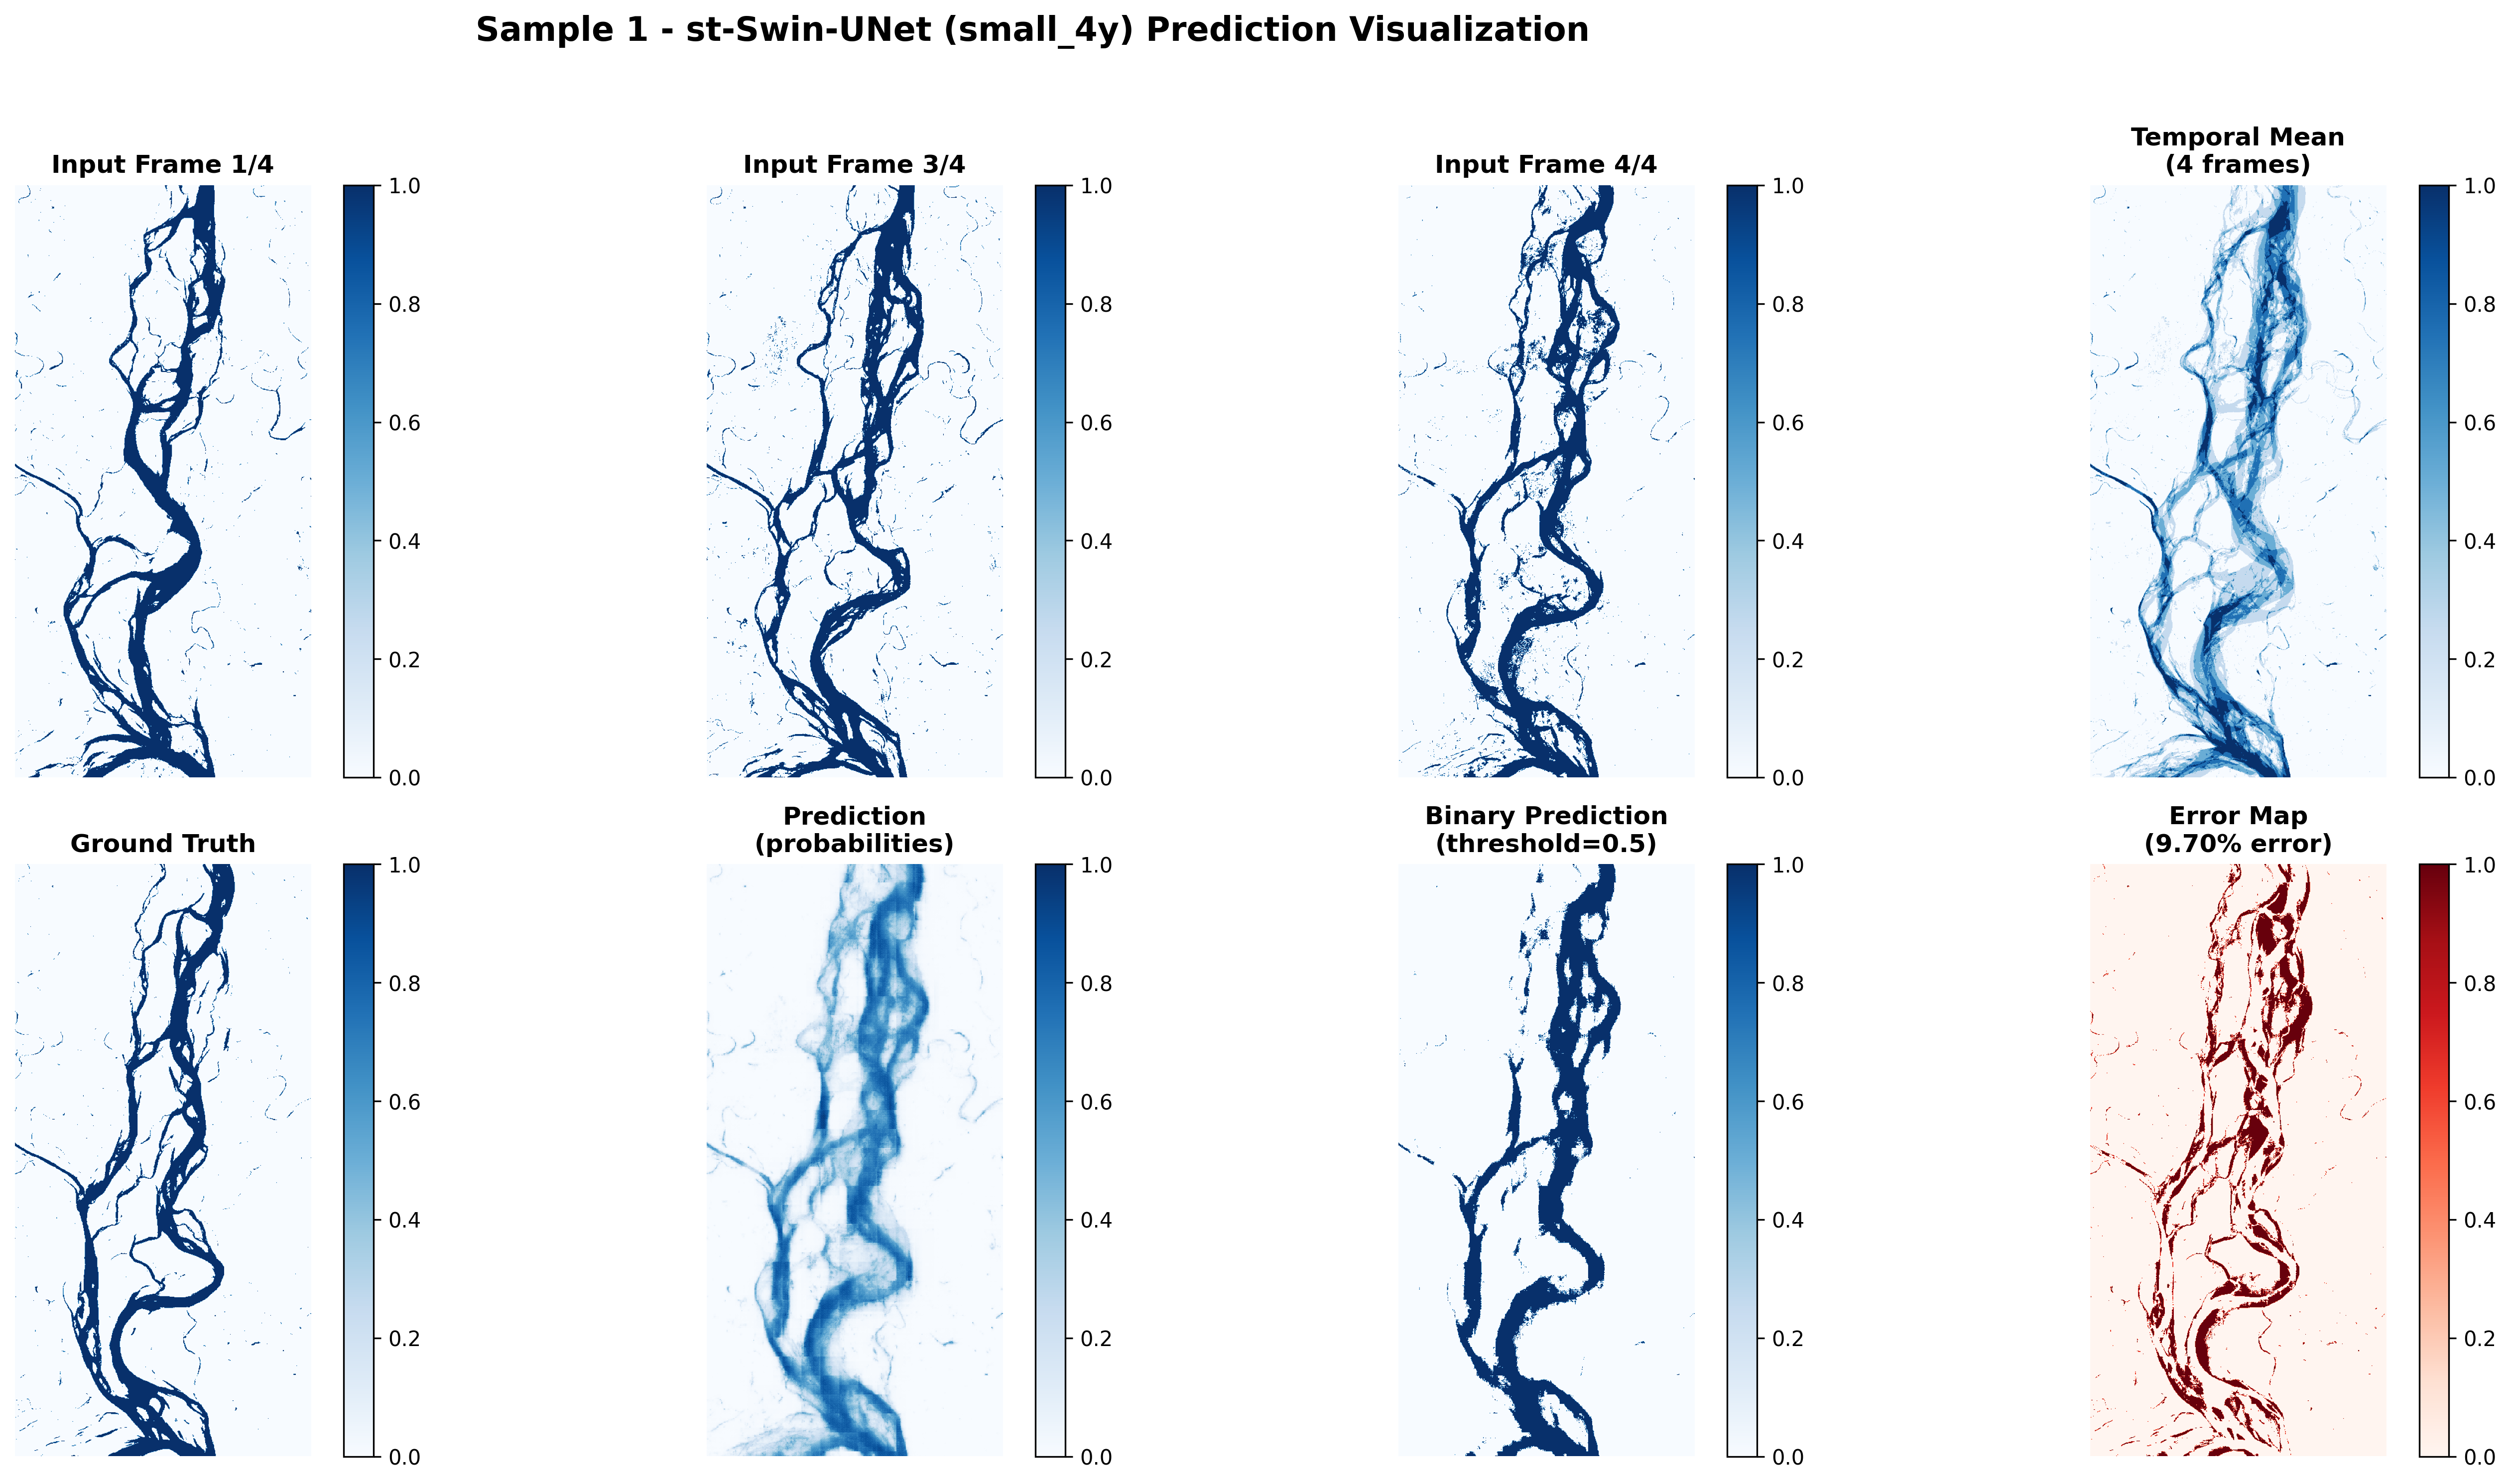
\includegraphics[width=0.6\linewidth]{figures/prediction_stswin_small_4y_sample001.png}
    \caption{st-Swin-UNet small variant prediction on test set (epoch $14$, $4$-year input).}
    \label{fig: st-Swin-UNet prediction}
\end{figure}

\begin{figure}[H]
    \centering
    \begin{subfigure}[b]{0.4\textwidth}
        \centering
        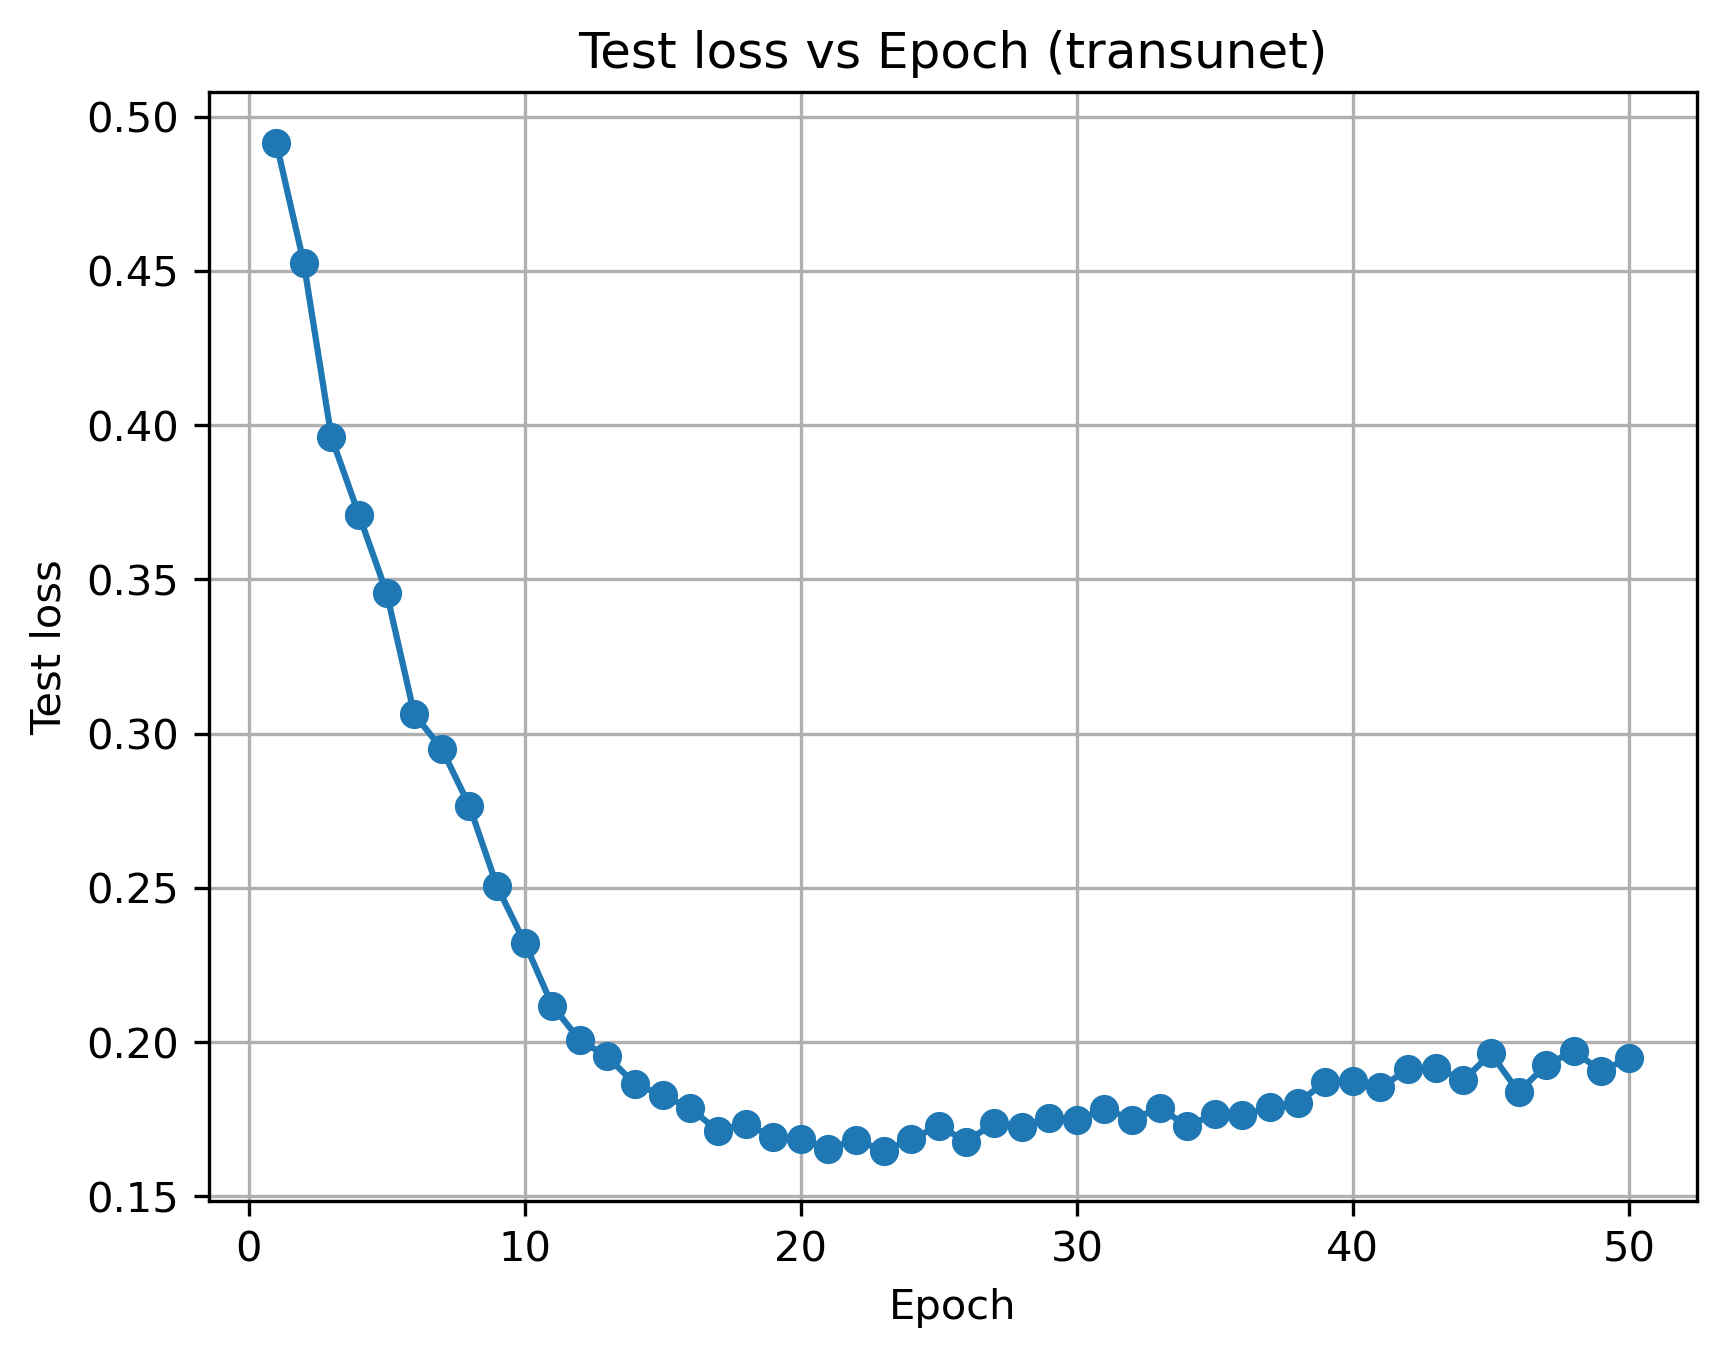
\includegraphics[width=\textwidth]{figures/test_loss_transunet_9years.png}
        \caption{TransUNet}
        \label{subfig: TransUNet 9 years test loss}
    \end{subfigure}
    \begin{subfigure}[b]{0.4\textwidth}
        \centering
        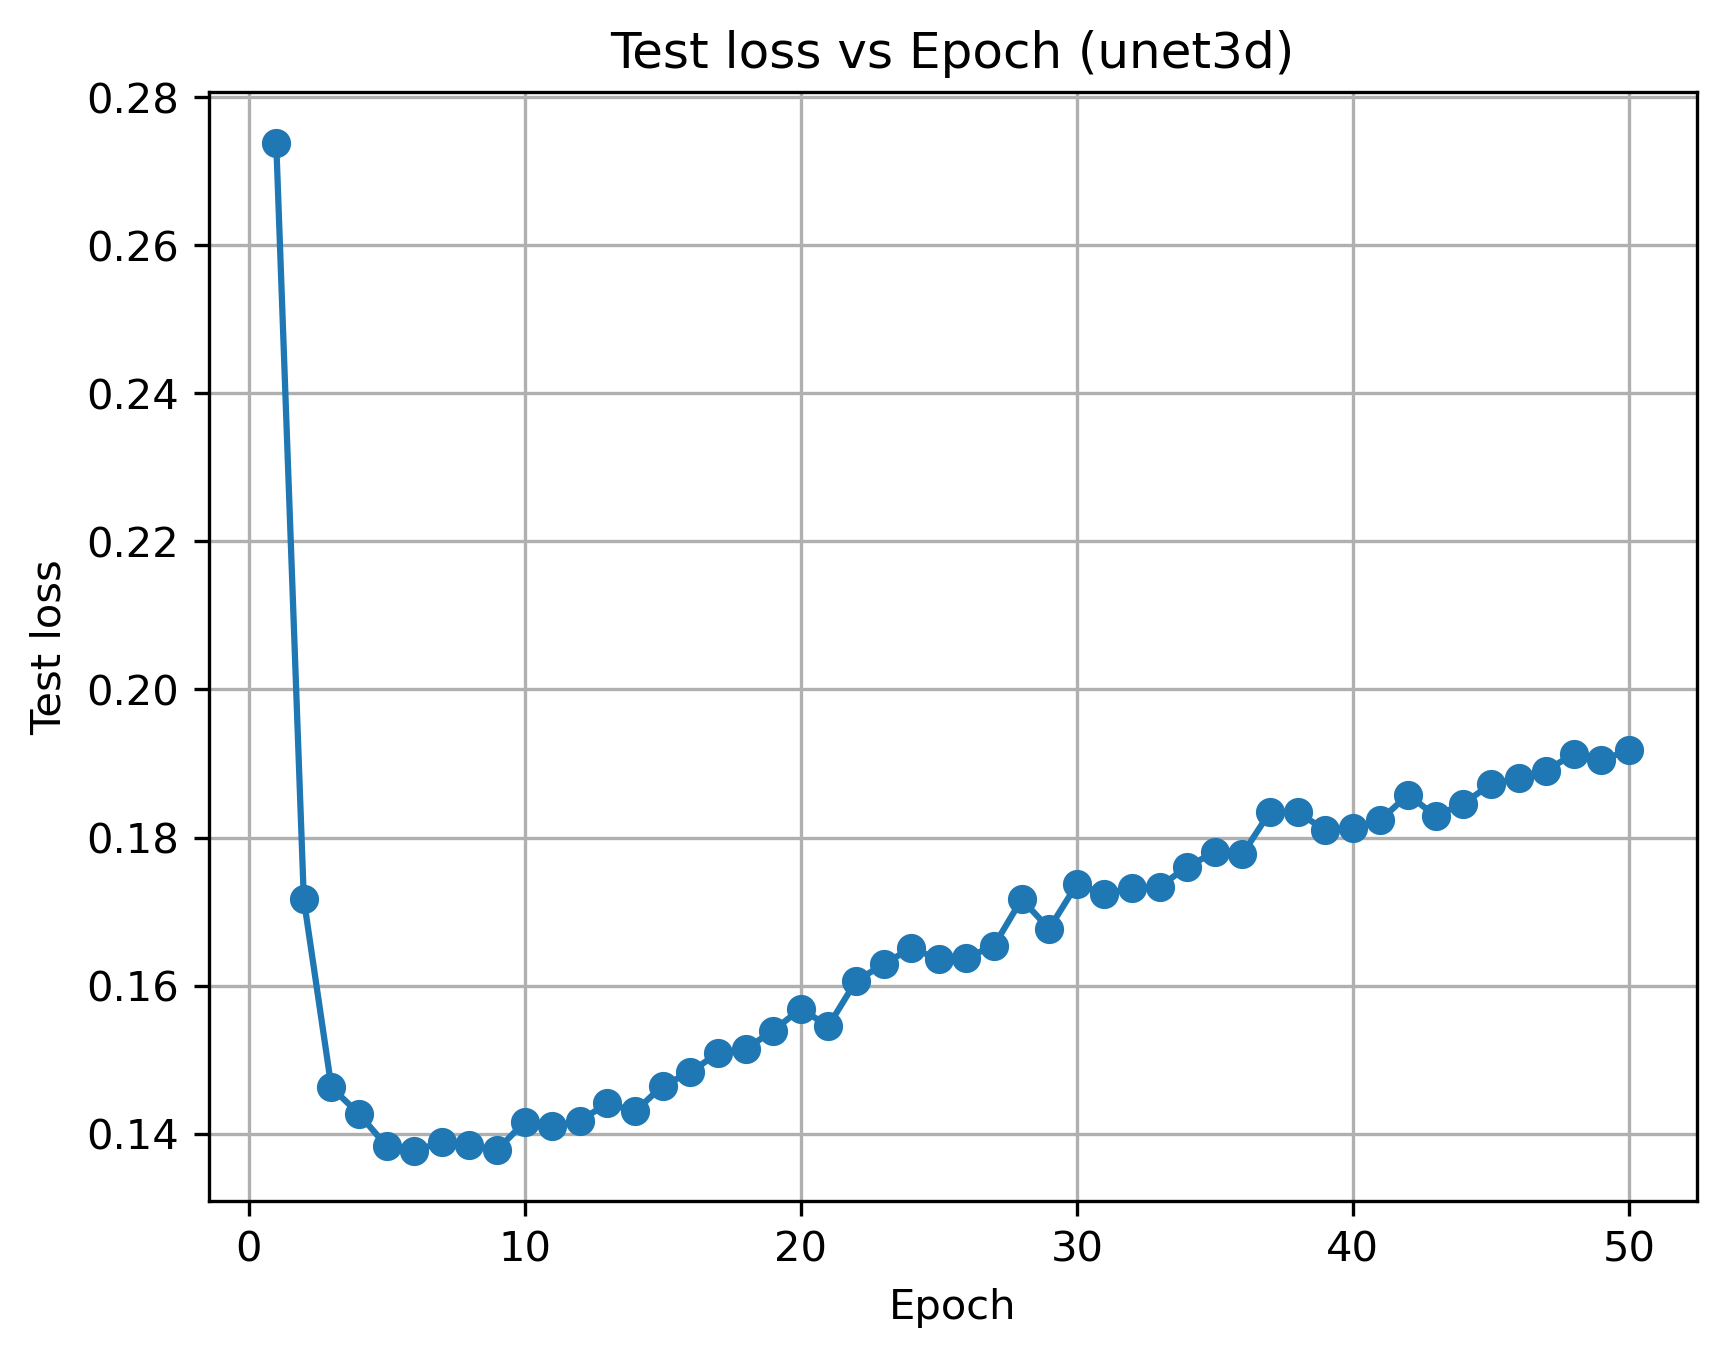
\includegraphics[width=\textwidth]{figures/test_loss_unet3d_9years.png}
        \caption{JamUNet}
        \label{subfig: JamUNet 9 years test loss}
    \end{subfigure}
    \caption{Variation of test loss against training epoch (9 year input).}
    \label{fig: TransUNet vs JamUNet 9 years test loss}
\end{figure}

\begin{figure}[H]
    \centering
    \begin{subfigure}[b]{0.4\textwidth}
        \centering
        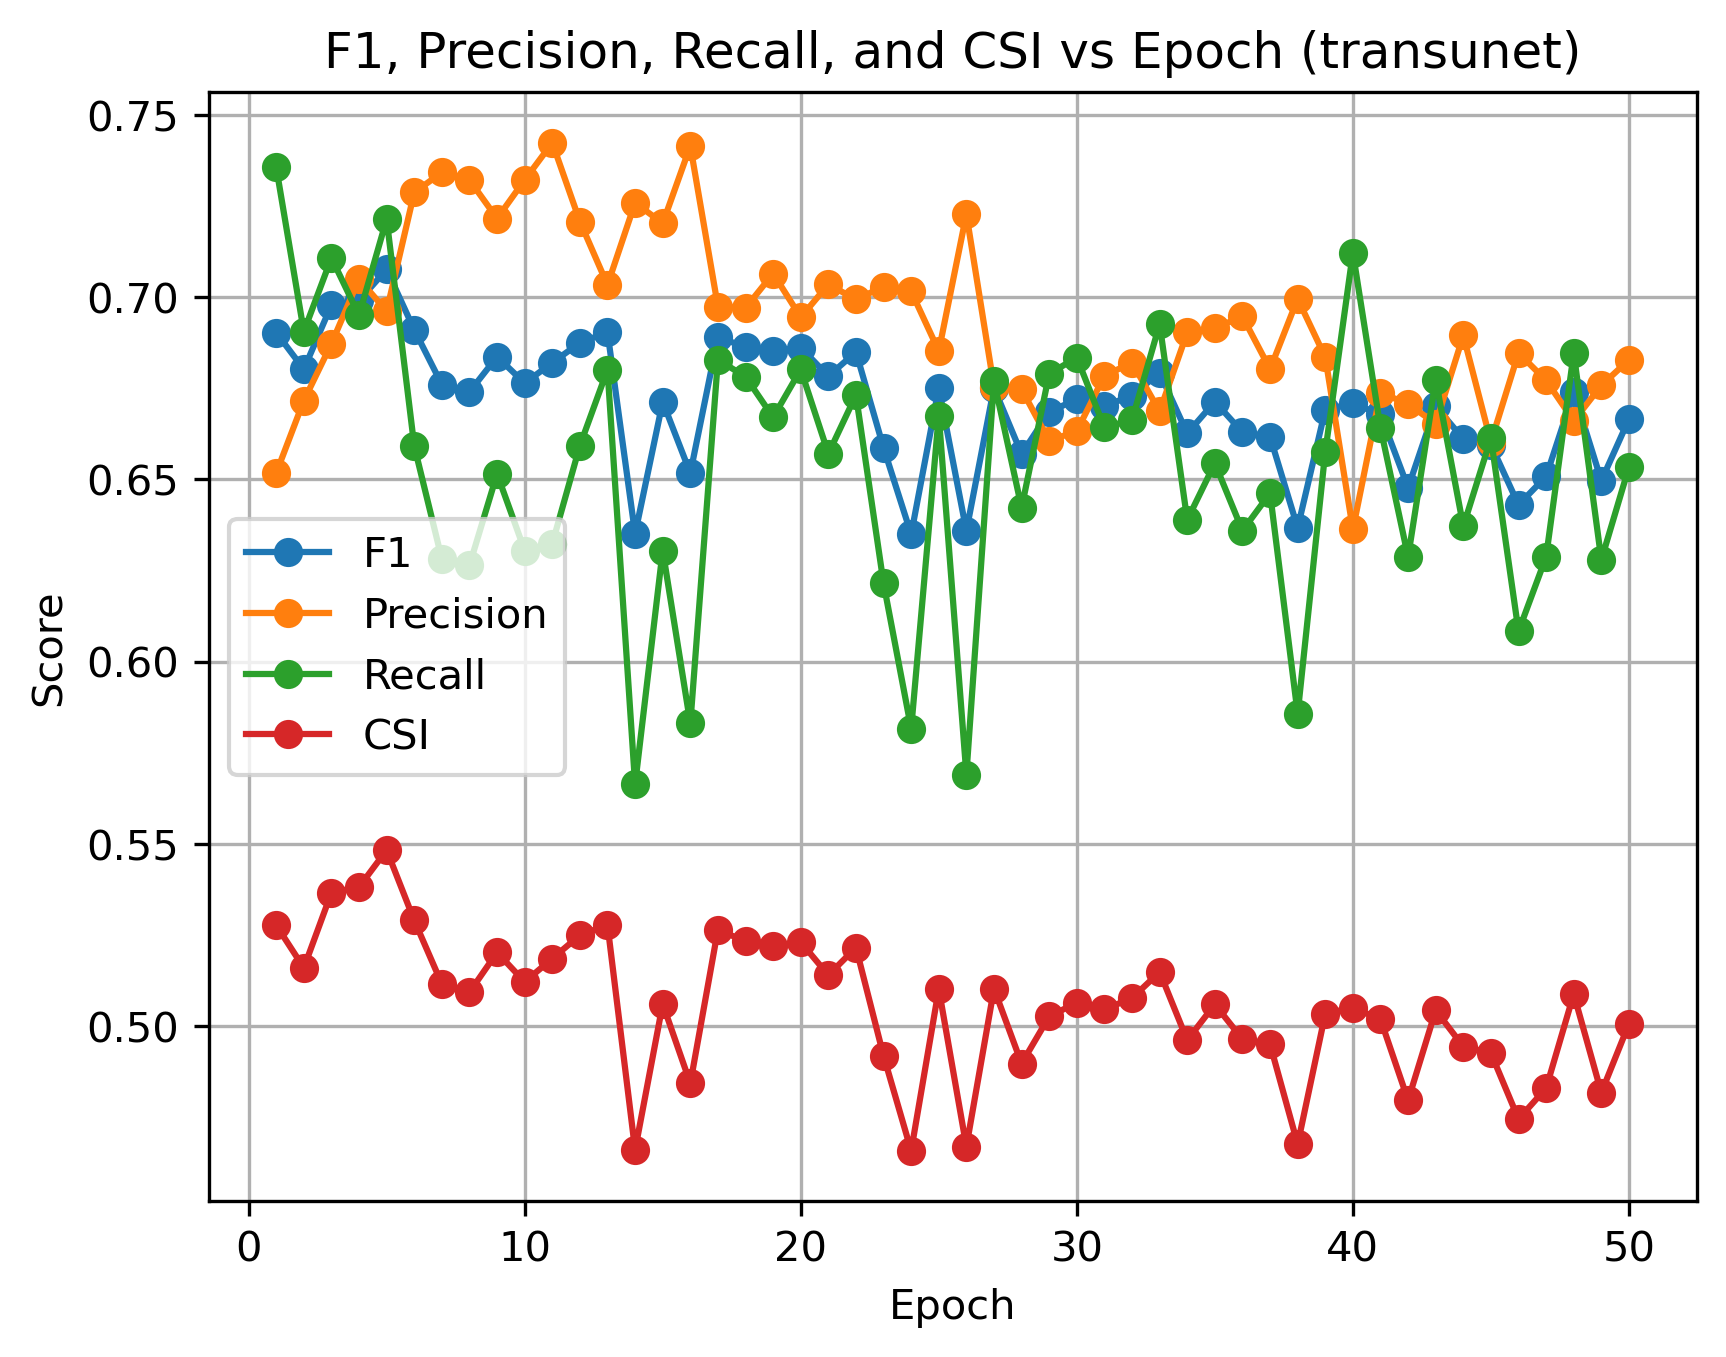
\includegraphics[width=\textwidth]{figures/test_scores_transunet_9years.png}
        \caption{TransUNet}
        \label{subfig: TransUNet 9 years scores}
    \end{subfigure}
    \begin{subfigure}[b]{0.4\textwidth}
        \centering
        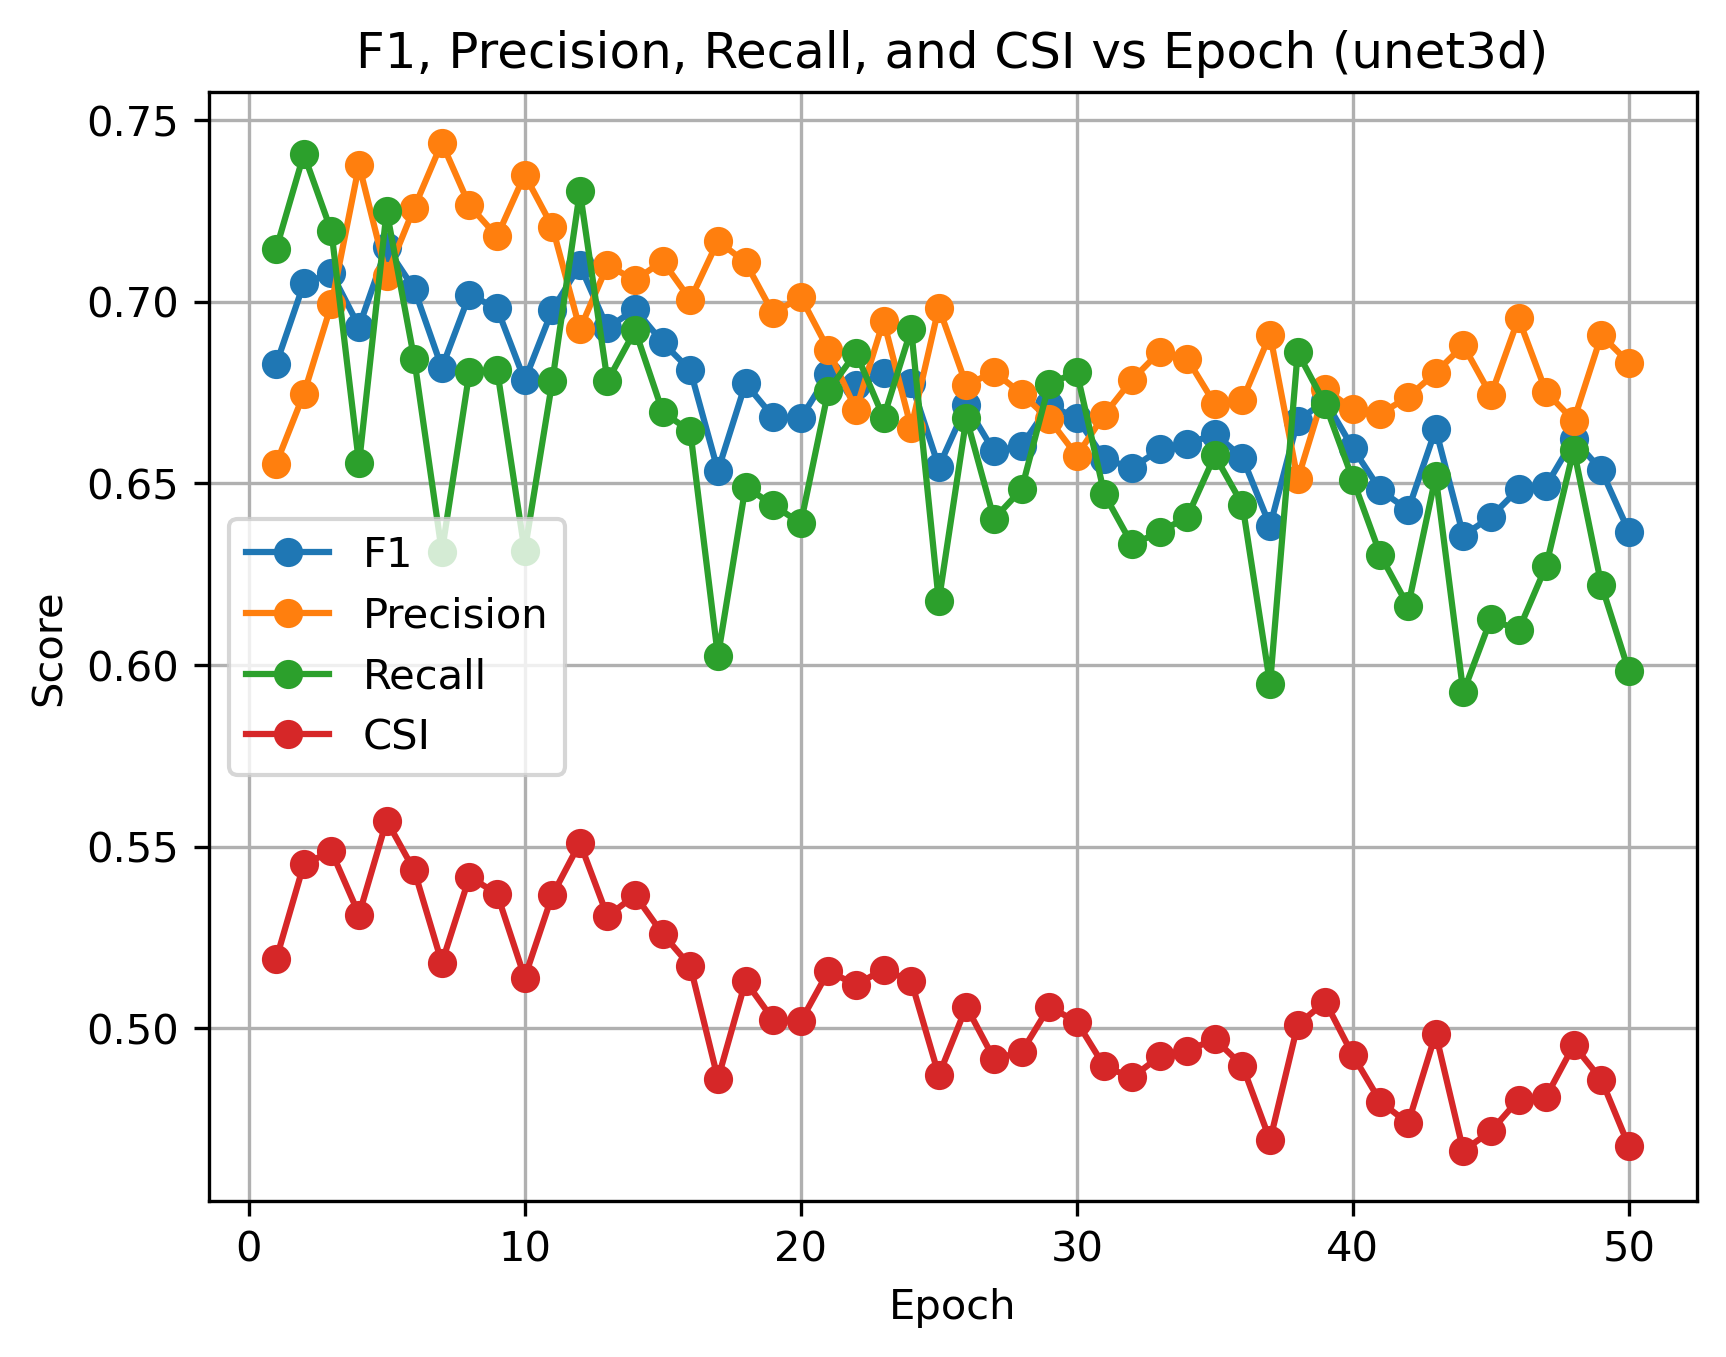
\includegraphics[width=\textwidth]{figures/test_scores_unet3d_9years.png}
        \caption{JamUNet}
        \label{subfig: JamUNet 9 years scores}
    \end{subfigure}
    \caption{F1, recall, precision, csi scores comparison between TransUNet and JamUNet models (9 year input).}
    \label{fig: TransUNet vs JamUNet 9 years scores comparison}
\end{figure}

\begin{figure}[H]
    \centering
    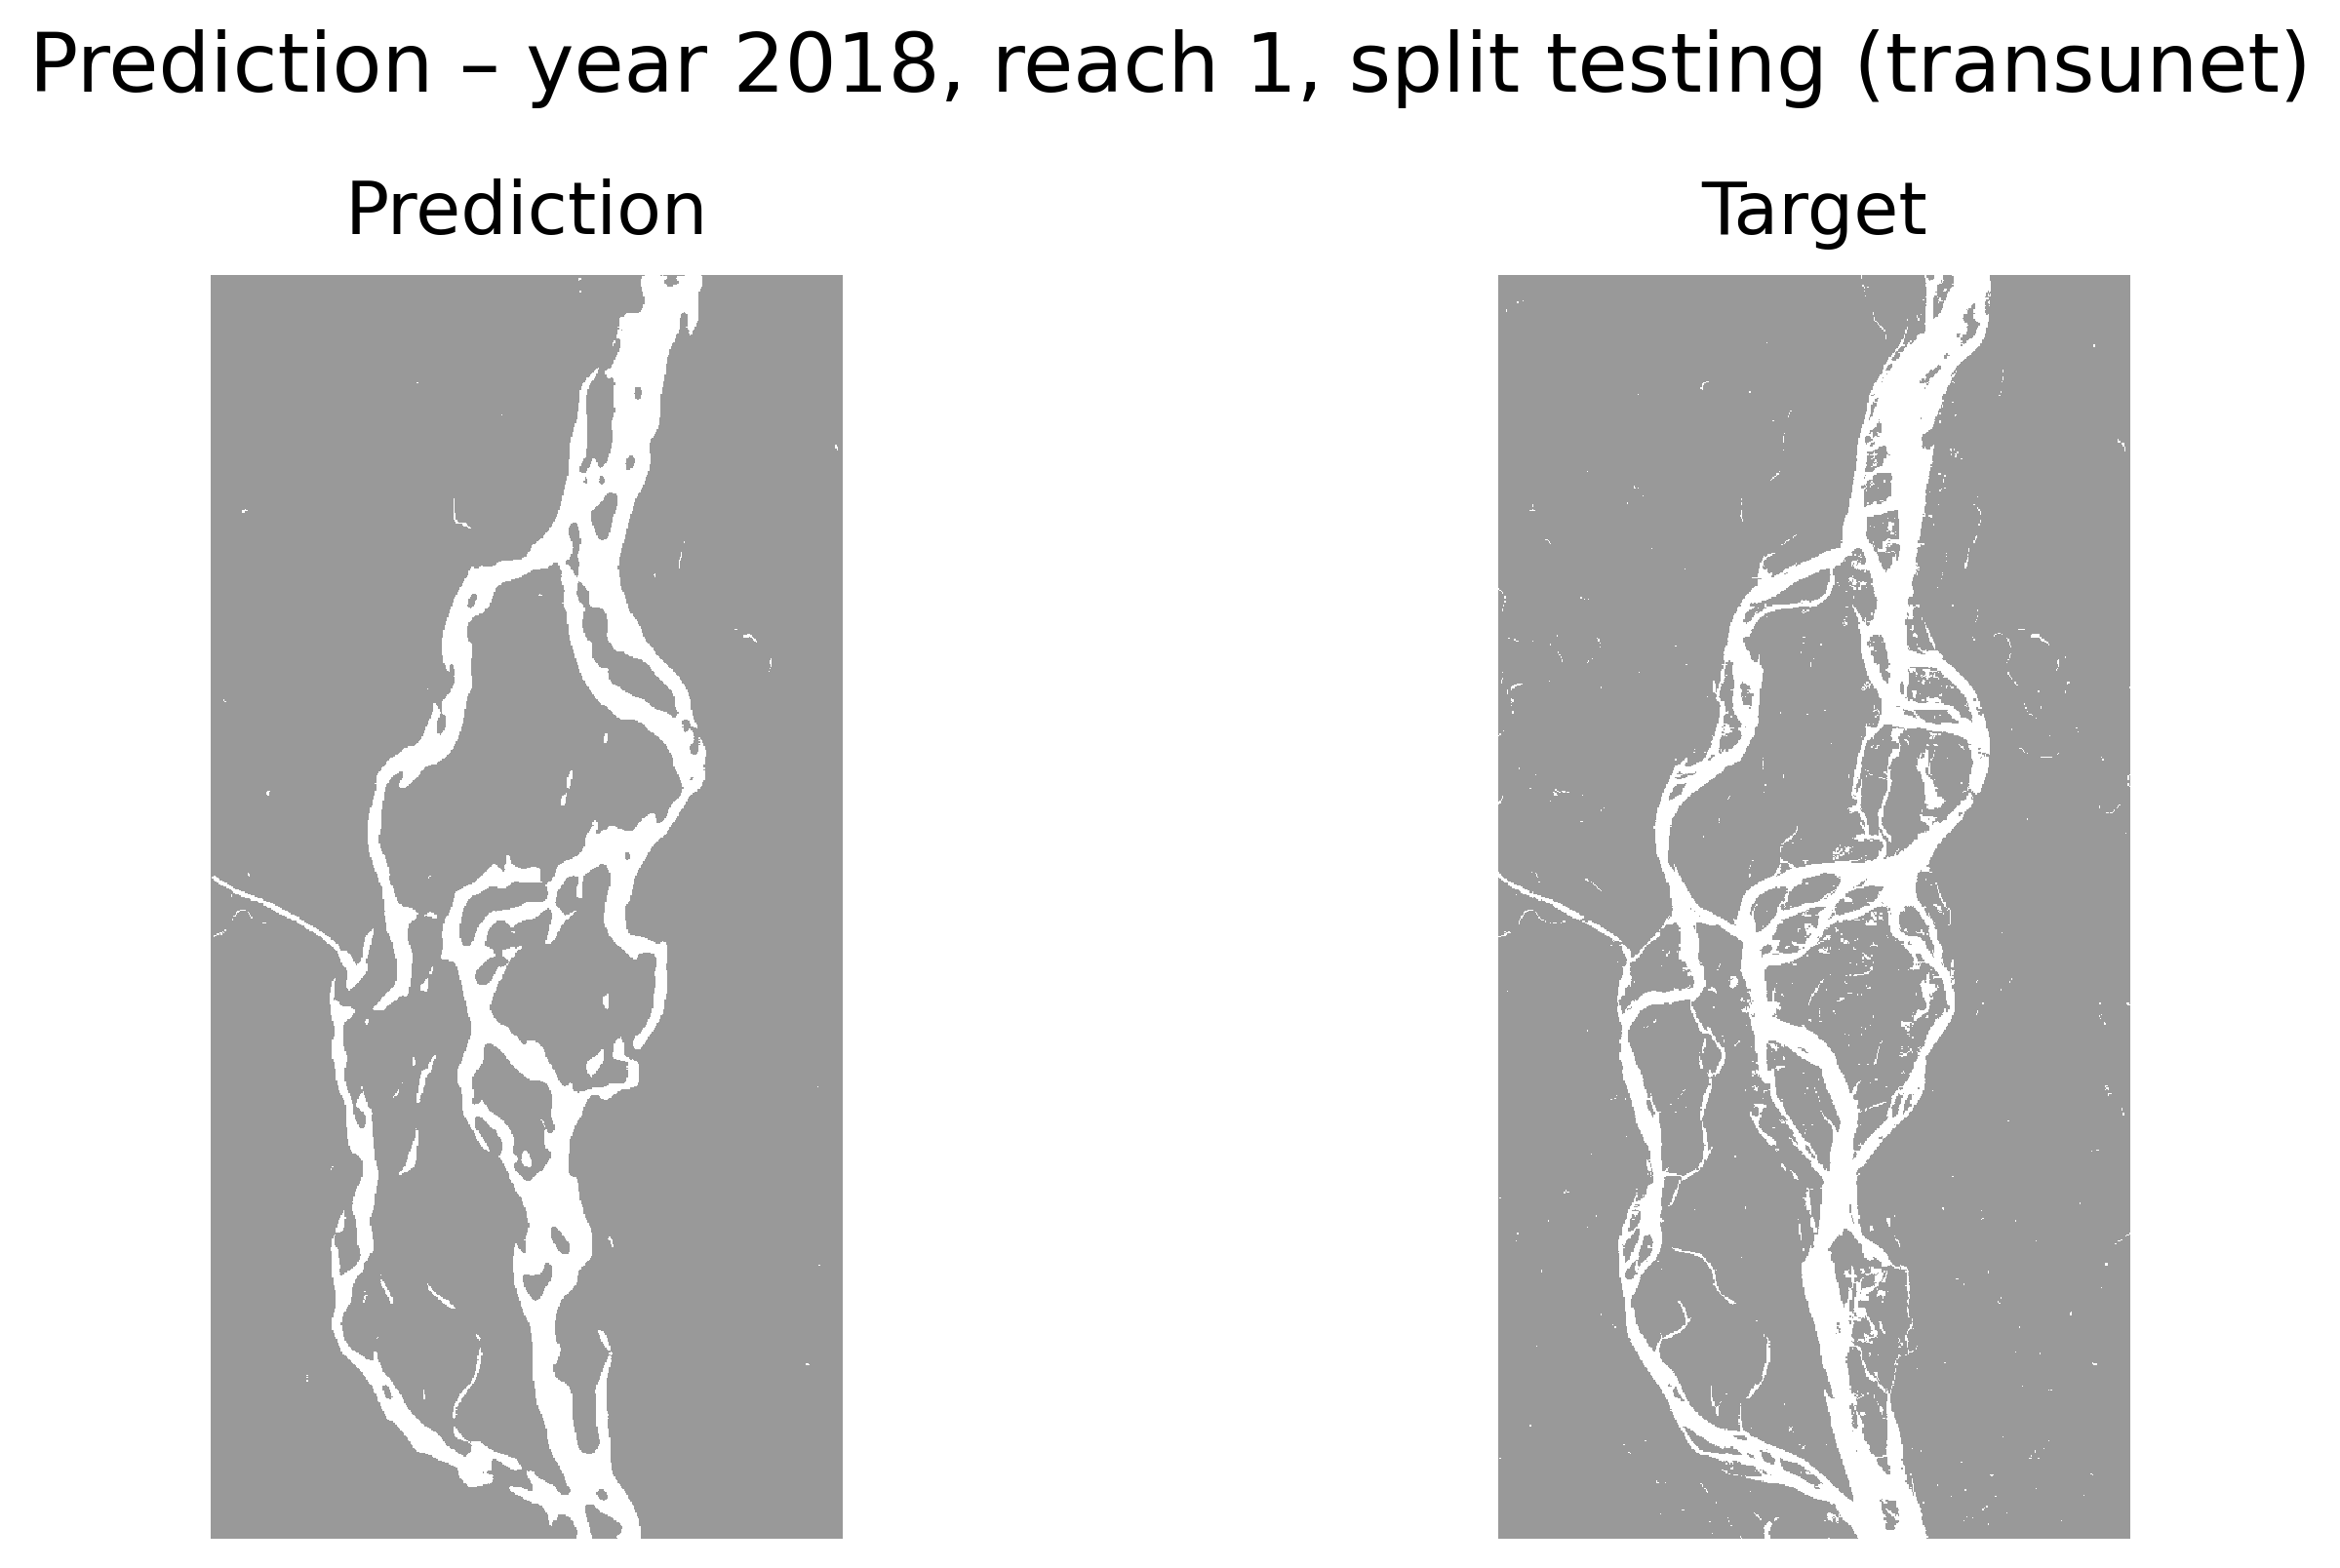
\includegraphics[width=0.6\linewidth]{figures/prediction_year2018_reach1_testing_transunet_9years_epoch033_predonly.png}
    \caption{TransUNet input sequence of years $2009-2017$, target year $2018$ for sample river location.}
    \label{fig: TransUNet 9 years prediction map}
\end{figure}

\begin{figure}[H]
    \centering
    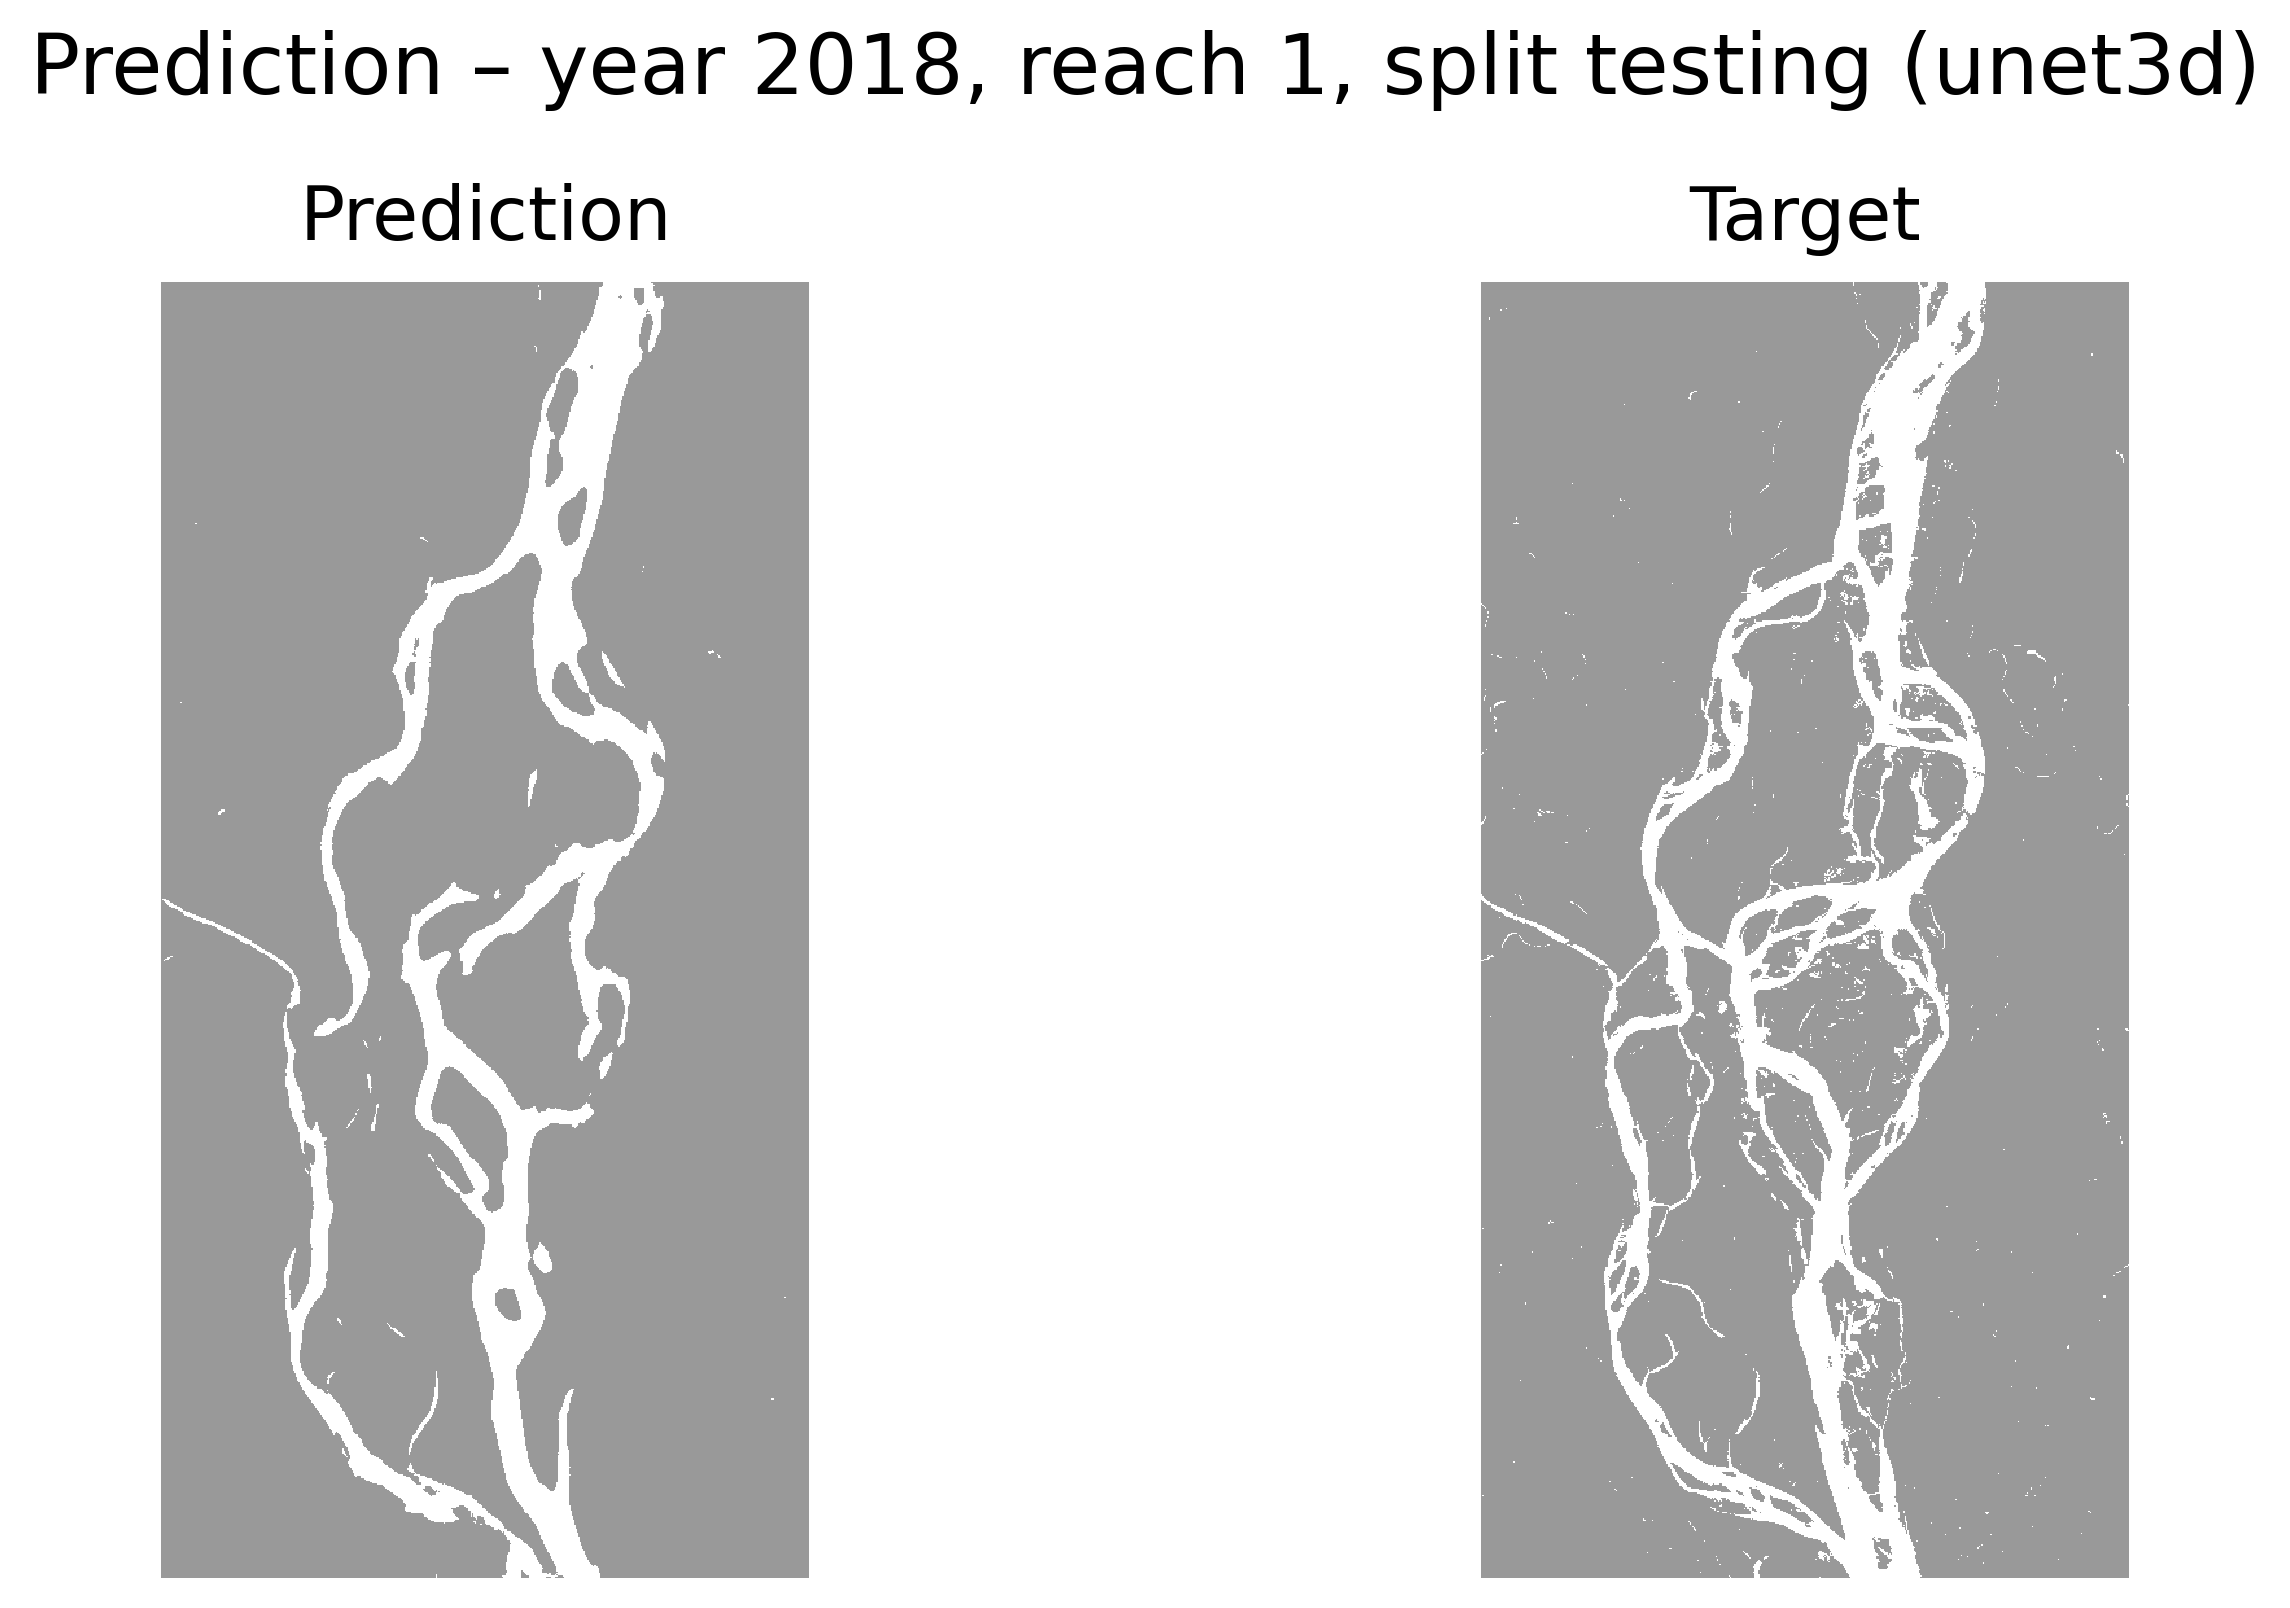
\includegraphics[width=0.6\linewidth]{figures/prediction_year2018_reach1_testing_unet3d_9years_epoch018_predonly.png}
    \caption{JamUNet input sequence of years $2009-2017$, target year $2018$ for sample river location.}
    \label{fig: JamUNet 9 years prediction map}
\end{figure}

\begin{figure}[H]
    \centering
    \begin{subfigure}[b]{0.495\textwidth}
        \centering
        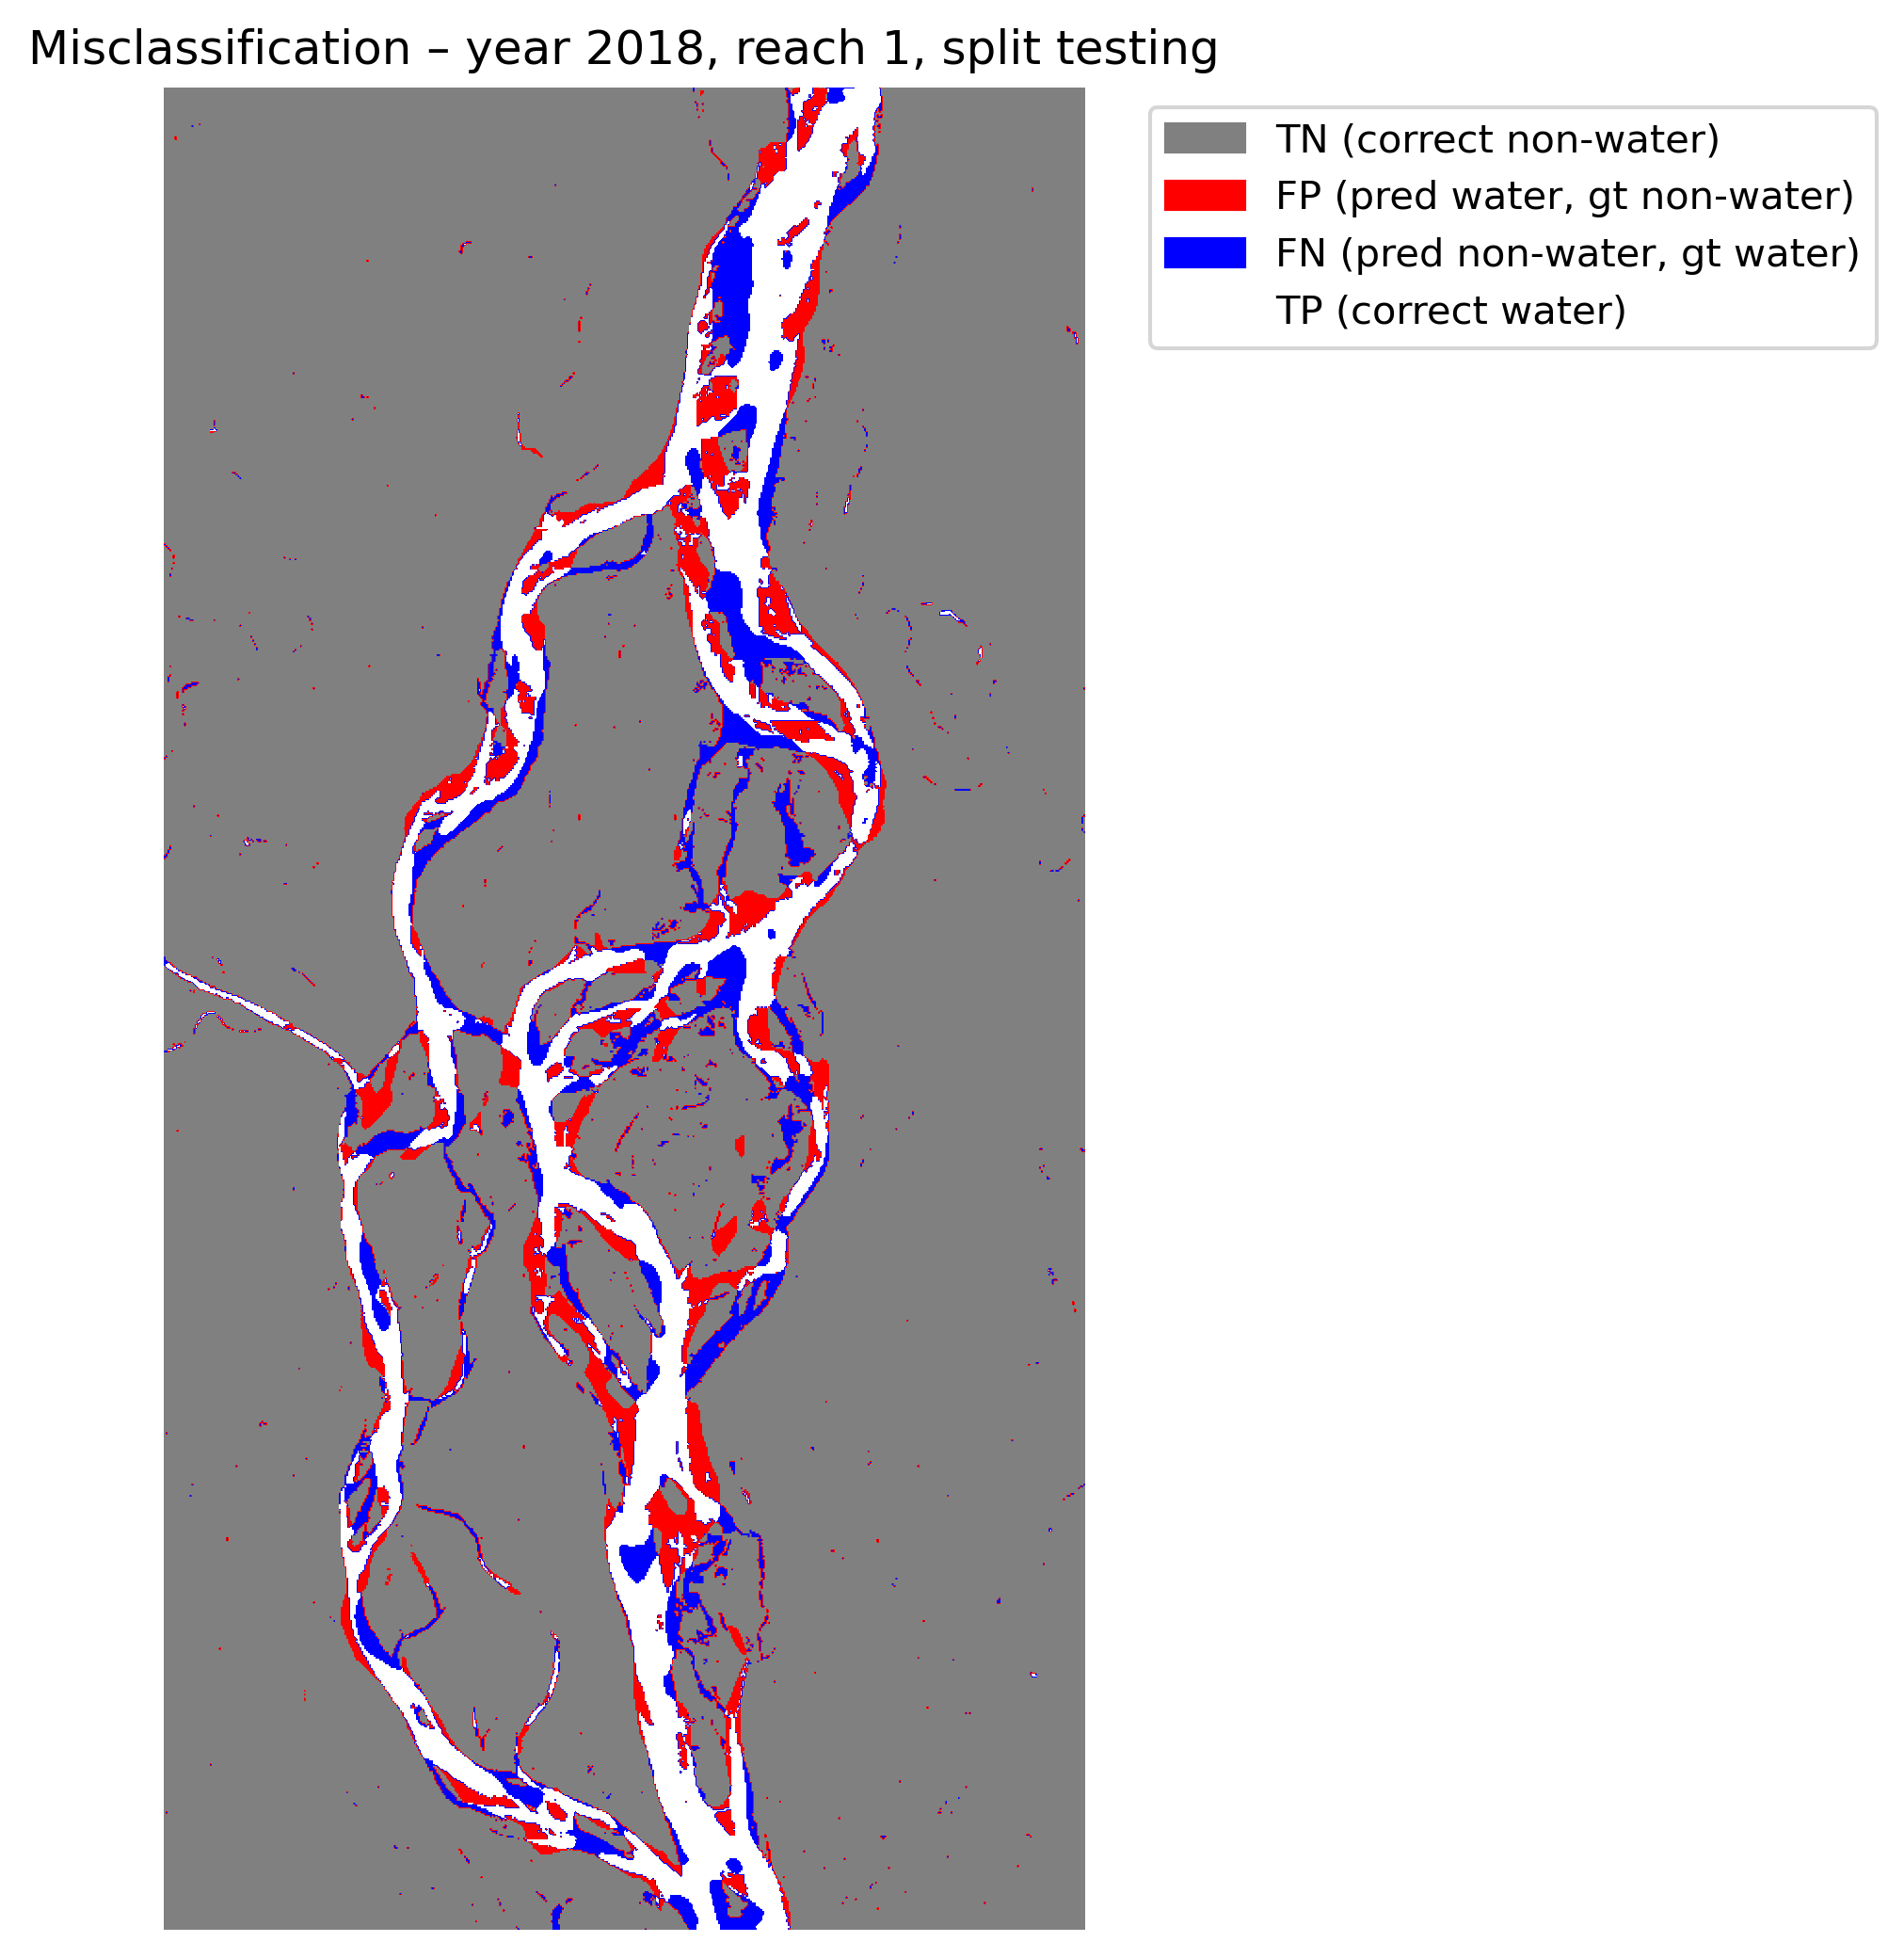
\includegraphics[width=\textwidth]{figures/misclass_year2018_reach1_testing_transunet_9years_epoch033.png}
        \caption{TransUNet}
        \label{subfig: TransUNet 9 years misclassification map}
    \end{subfigure}
    \begin{subfigure}[b]{0.495\textwidth}
        \centering
        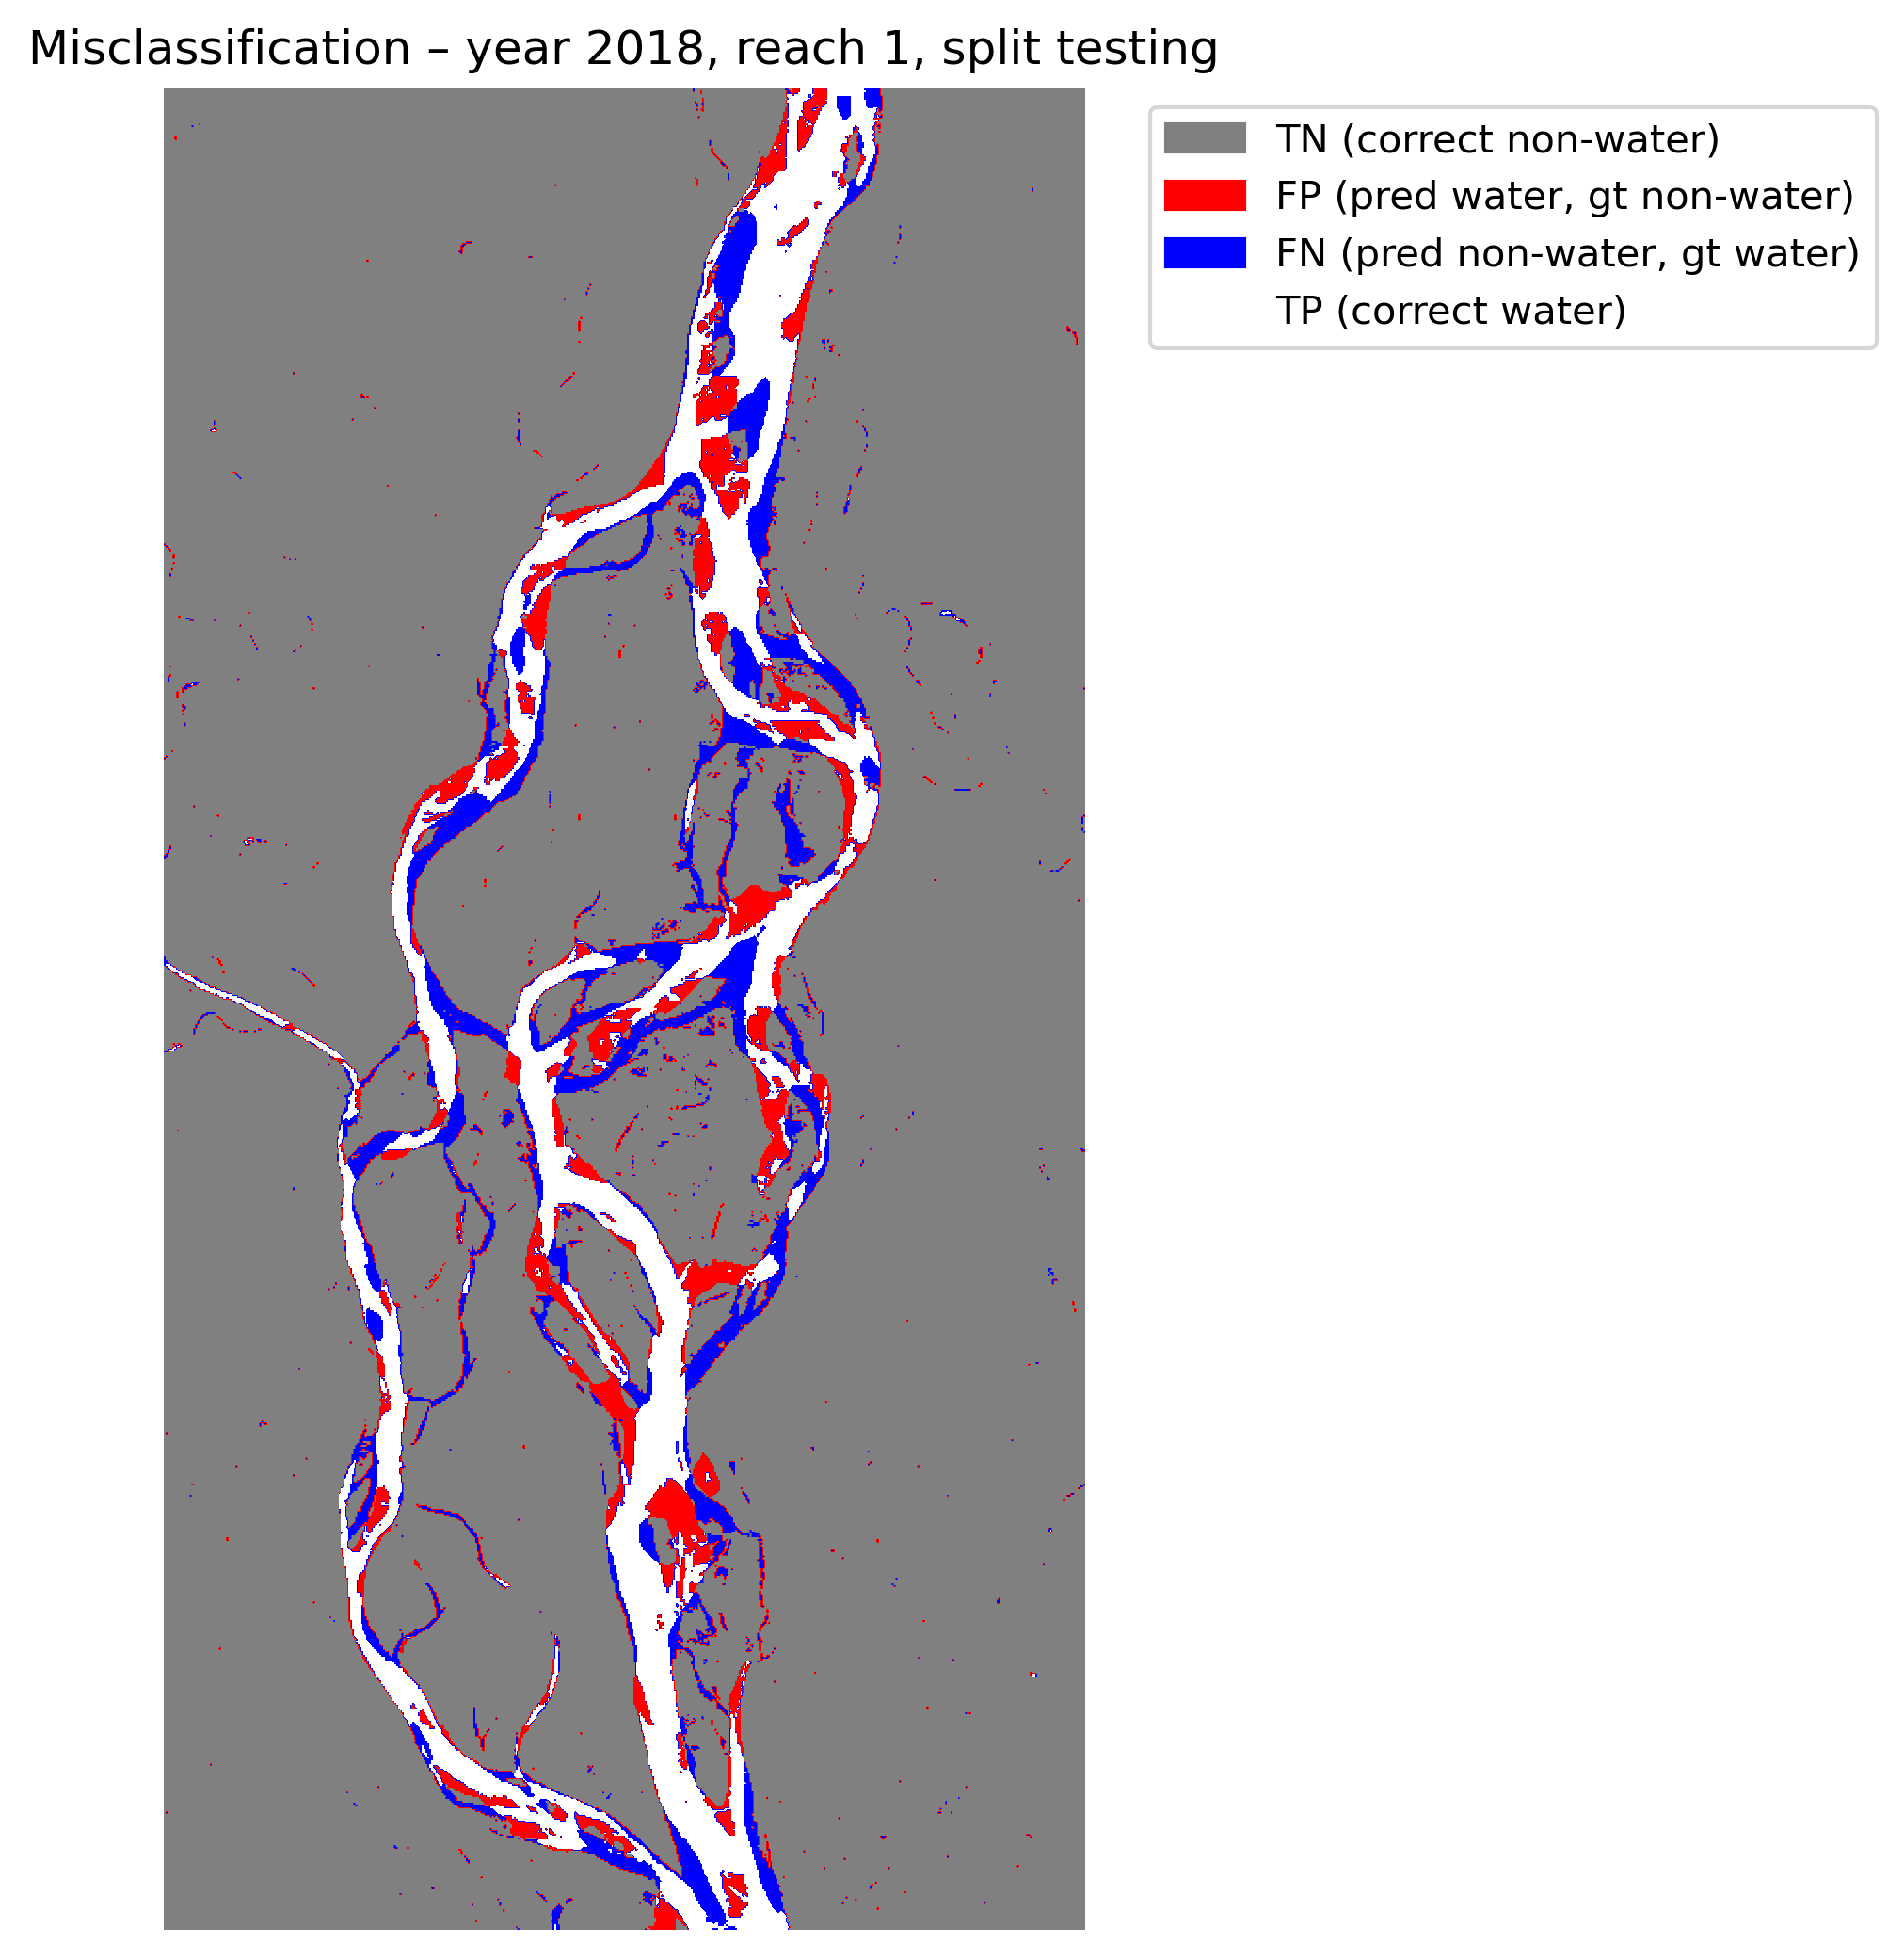
\includegraphics[width=\textwidth]{figures/misclass_year2018_reach1_testing_unet3d_9years_epoch018.png}
        \caption{JamUNet}
        \label{subfig: JamUNet 9 years misclassification map}
    \end{subfigure}
    \caption{Misclassification map comparison between TransUNet and JamUNet models on a selected test image (9 year input).}
    \label{fig: TransUNet vs JamUNet 9 years misclassification map}
\end{figure}



\end{document}